\frame{
	\begin{tikzpicture}[remember picture,overlay]
	\fill[blue1]
	(current page.north west) rectangle ([xshift=12.cm,yshift=-10.cm]current page.east|-{pic cs:end});
	\end{tikzpicture}
	\begin{textblock}{0.9}(0.05,0.15)
		\centering
			{\huge
			\textcolor{white}{
			Measuring granular dynamics with}}\\[0.2cm]
		{\Huge
			\textcolor{white}{
			X-ray Digital Fourier Analysis (X-DFA)}}
	\end{textblock}

	\begin{textblock}{0.9}(0.05,0.45)
		\centering
		\movie[width =0.25\textwidth, poster, loop]
		{
\includegraphics[width=0.25\textwidth]{Sources/X-DFA/cropped_80kV_340uA_38ms_0000.png}}
		{Sources/X-DFA/3500mul_per_min_cropped_roi_512x512.avi}
	\end{textblock}
	
	\begin{textblock}{0.9}(0.05,0.93)
		\centering
		{
		\textcolor{white}{
		In collaboration with M.\ Escobedo \& S.\ Egelhaaf, University of Düsseldorf}}
	\end{textblock}
}


\frame{
\begin{tikzpicture}[remember picture,overlay]
\fill[blue1]
(current page.north west) rectangle ([xshift=0.52\paperwidth,yshift=0.33\paperheight]current page.west|-{pic cs:end});
\end{tikzpicture}

\begin{textblock}{0.6}(0.02,0.03)
	\textcolor{white}{
		\Large Experiments: A liquid fluidized bed}
\end{textblock}

\begin{textblock}{0.6}(0.03,0.12)
	\visible<1->{
	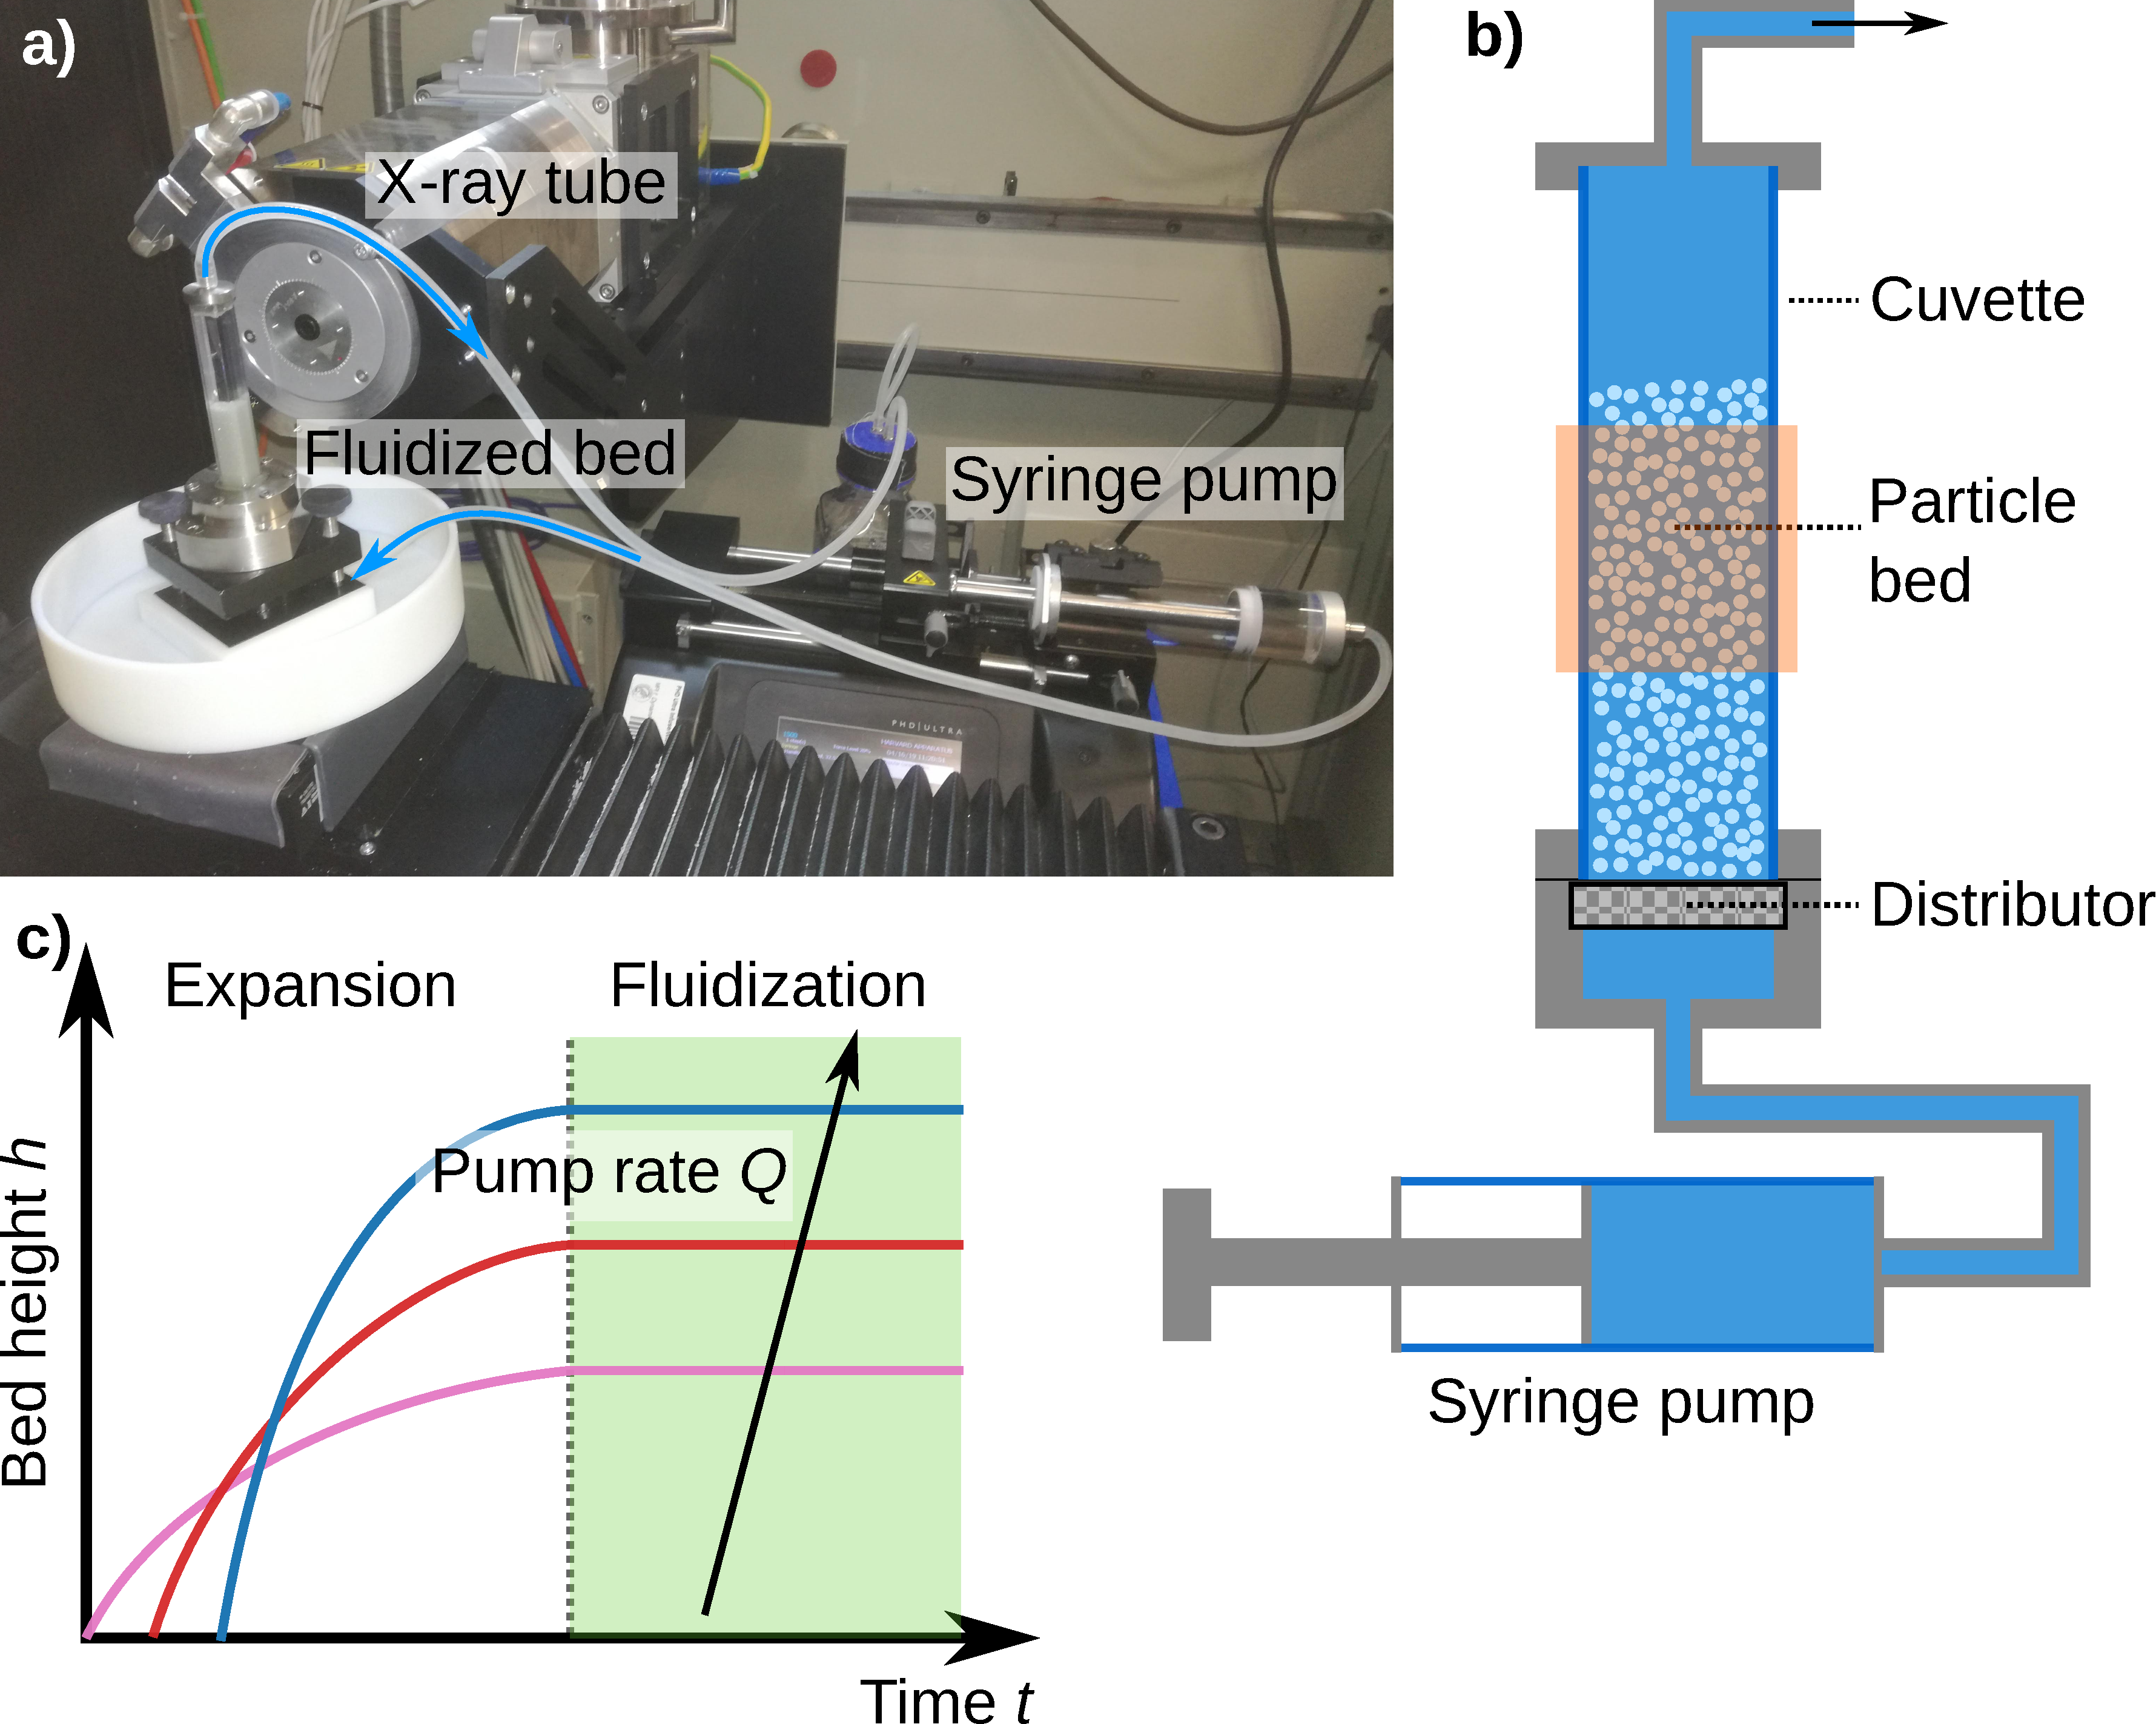
\includegraphics[width=\textwidth]{Sources/X-DFA/experiment-fluidized_bed_1.pdf}}
\end{textblock}

\begin{textblock}{0.6}(0.4,0.9)
	$0.45 < \Phi < 0.56$
\end{textblock}


\begin{textblock}{0.3}(0.65,0.1)
	\centering
	\only<1>{
		Radiogram\\
		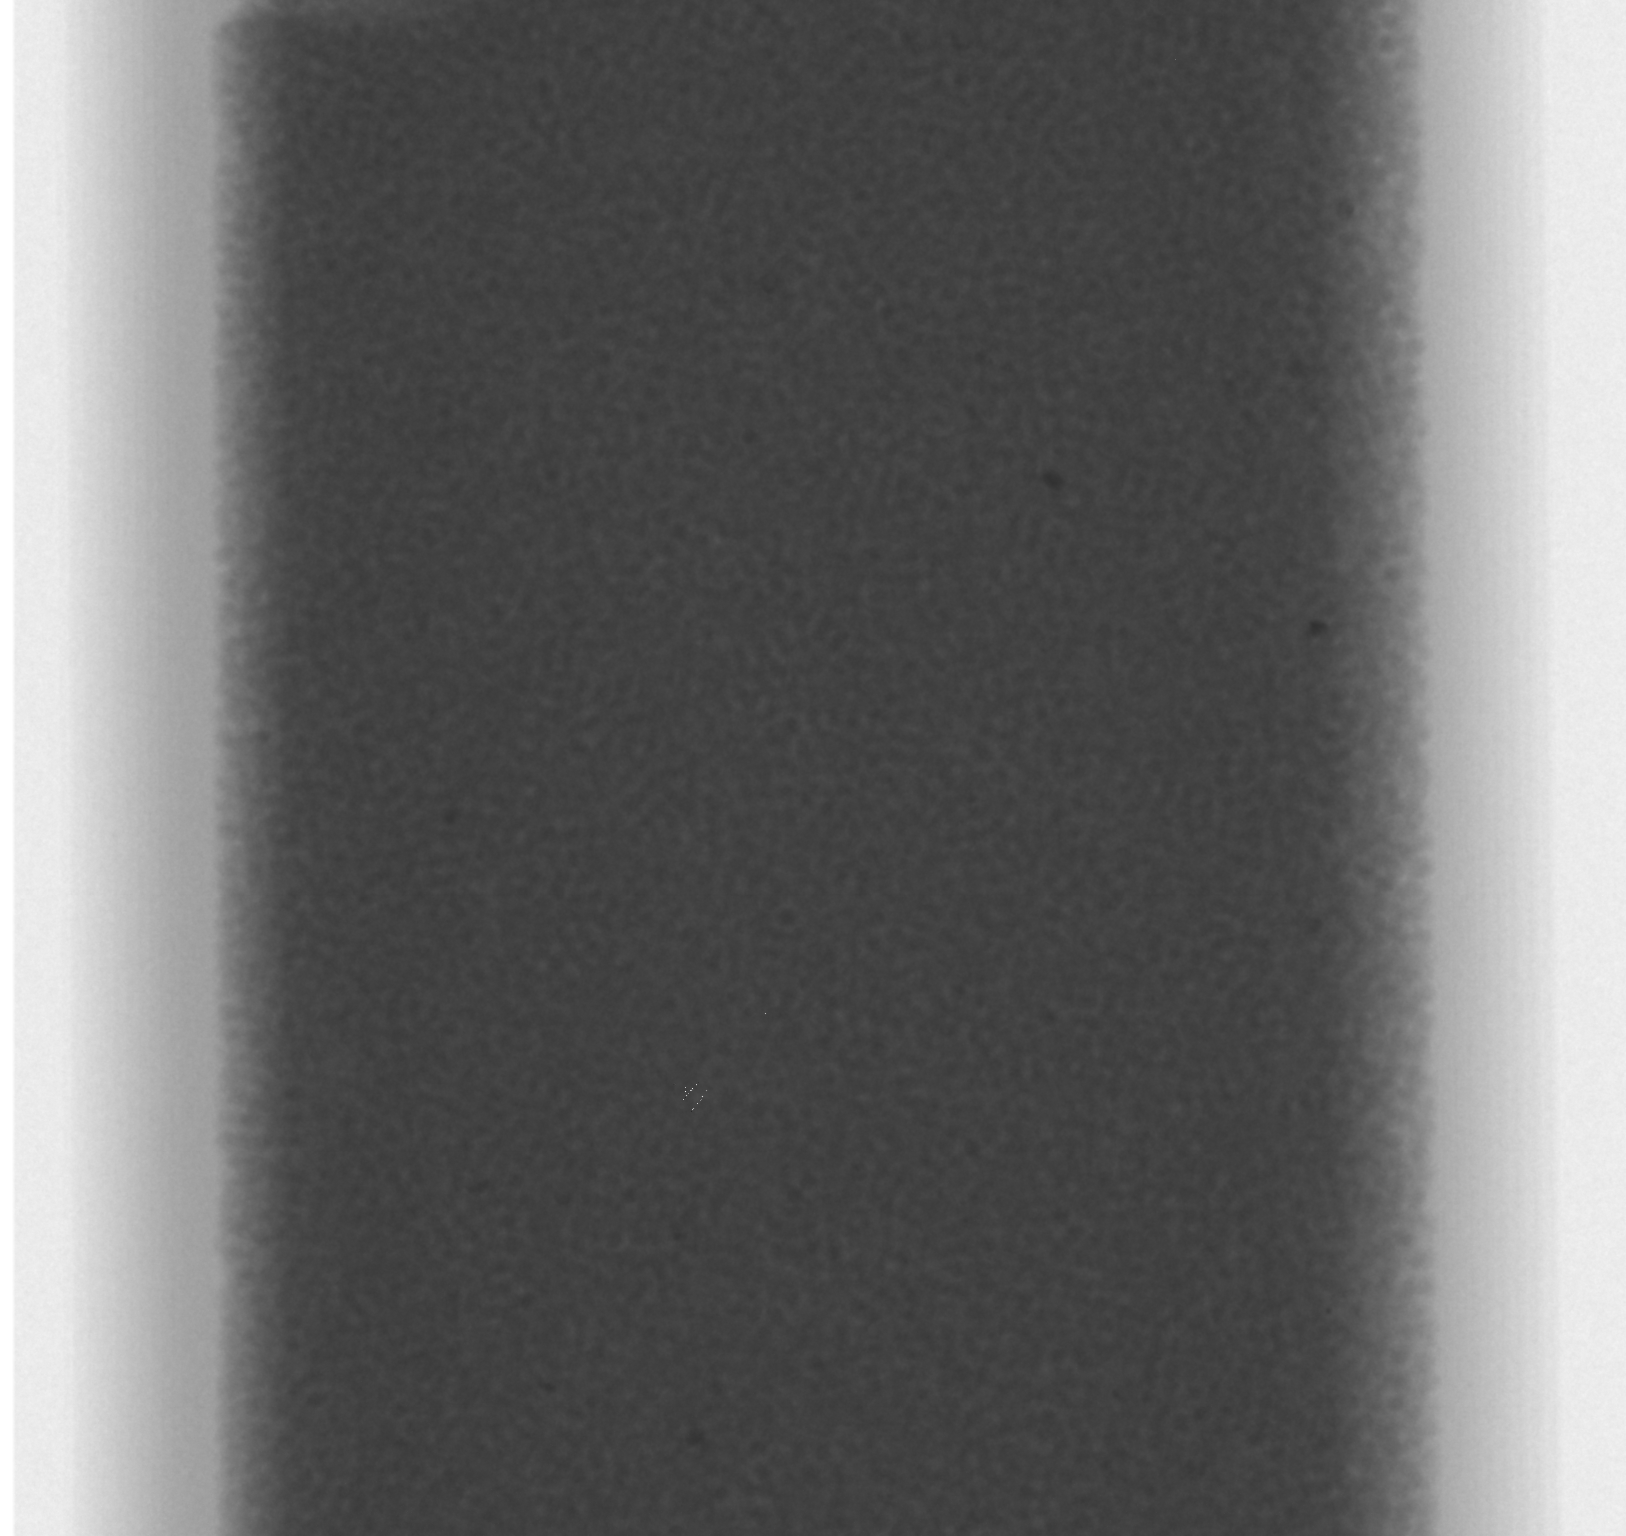
\includegraphics[width=\textwidth]{Sources/X-DFA/radiogram.png}}
\end{textblock}		

\begin{textblock}{0.3}(0.65,0.05)
	\visible<2->{
	\centering
	Particle tracking
	\fbox{
	\movie[width =\textwidth]
	{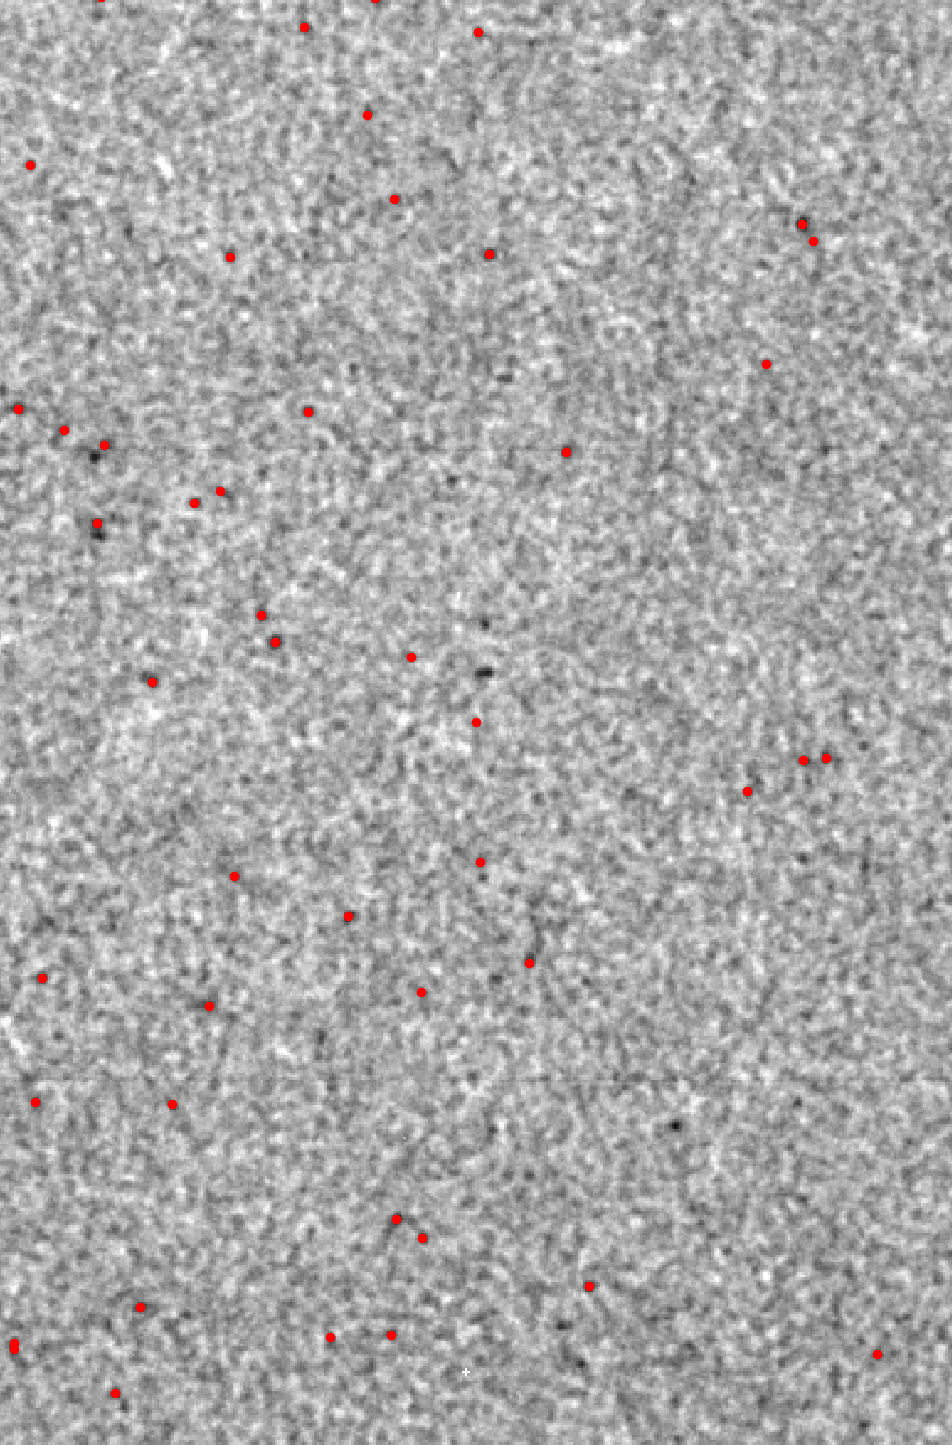
\includegraphics[width=\textwidth]{Sources/X-DFA/centroid_bronze_tracer_frame_nr_0000.png}}
	{Sources/X-DFA/centroid_bronze_tracer_4.mp4}}
	}
\end{textblock}
}

\begin{frame}[noframenumbering]
\begin{tikzpicture}[remember picture,overlay]
\fill[blue1]
(current page.north west) rectangle ([xshift=0.51\paperwidth,yshift=0.33\paperheight]current page.west|-{pic cs:end});
\end{tikzpicture}

\begin{textblock}{0.6}(0.02,0.03)
	\textcolor{white}{
		\Large Experiments: A liquid fluidized bed}
\end{textblock}

\begin{textblock}{0.6}(0.03,0.12)
	\visible<1->{
		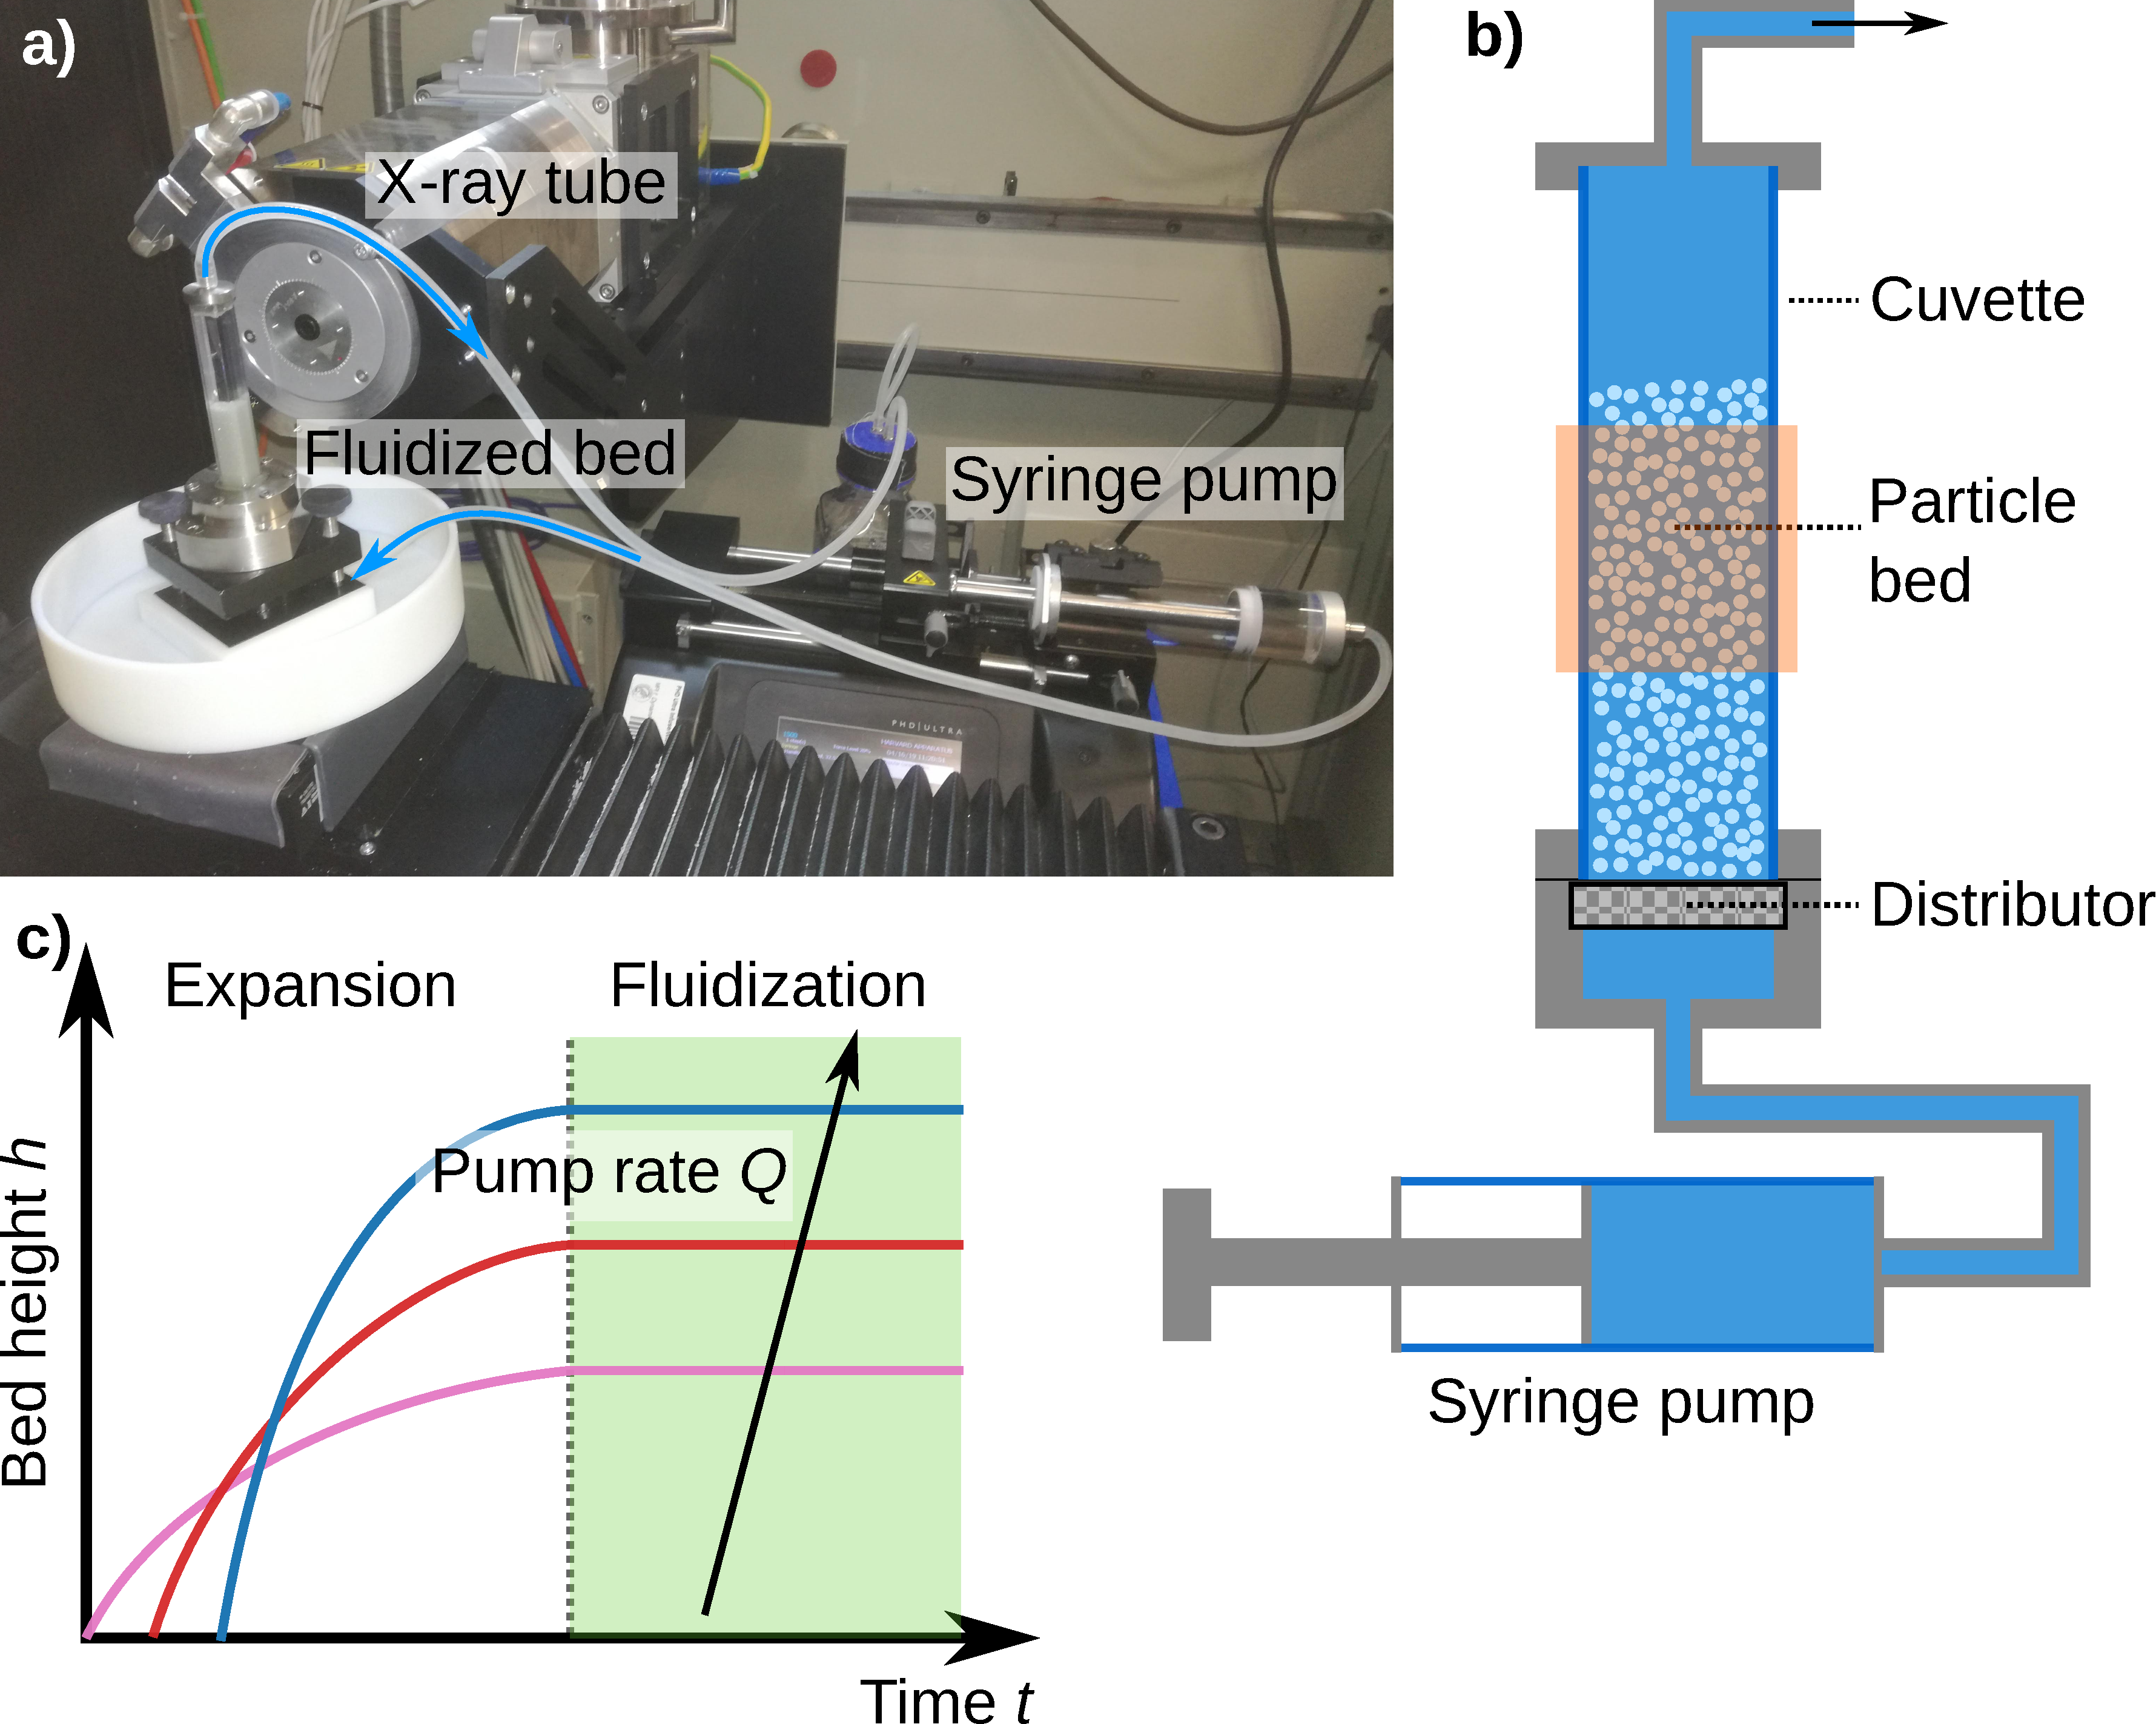
\includegraphics[width=\textwidth]{Sources/X-DFA/experiment-fluidized_bed_1.pdf}}
\end{textblock}

\begin{textblock}{0.6}(0.42,0.9)
	$0.45 < \Phi < 0.56$
\end{textblock}


\begin{textblock}{0.3}(0.65,0.03)
	\centering
	\only<1>{
		Radiogram\\
		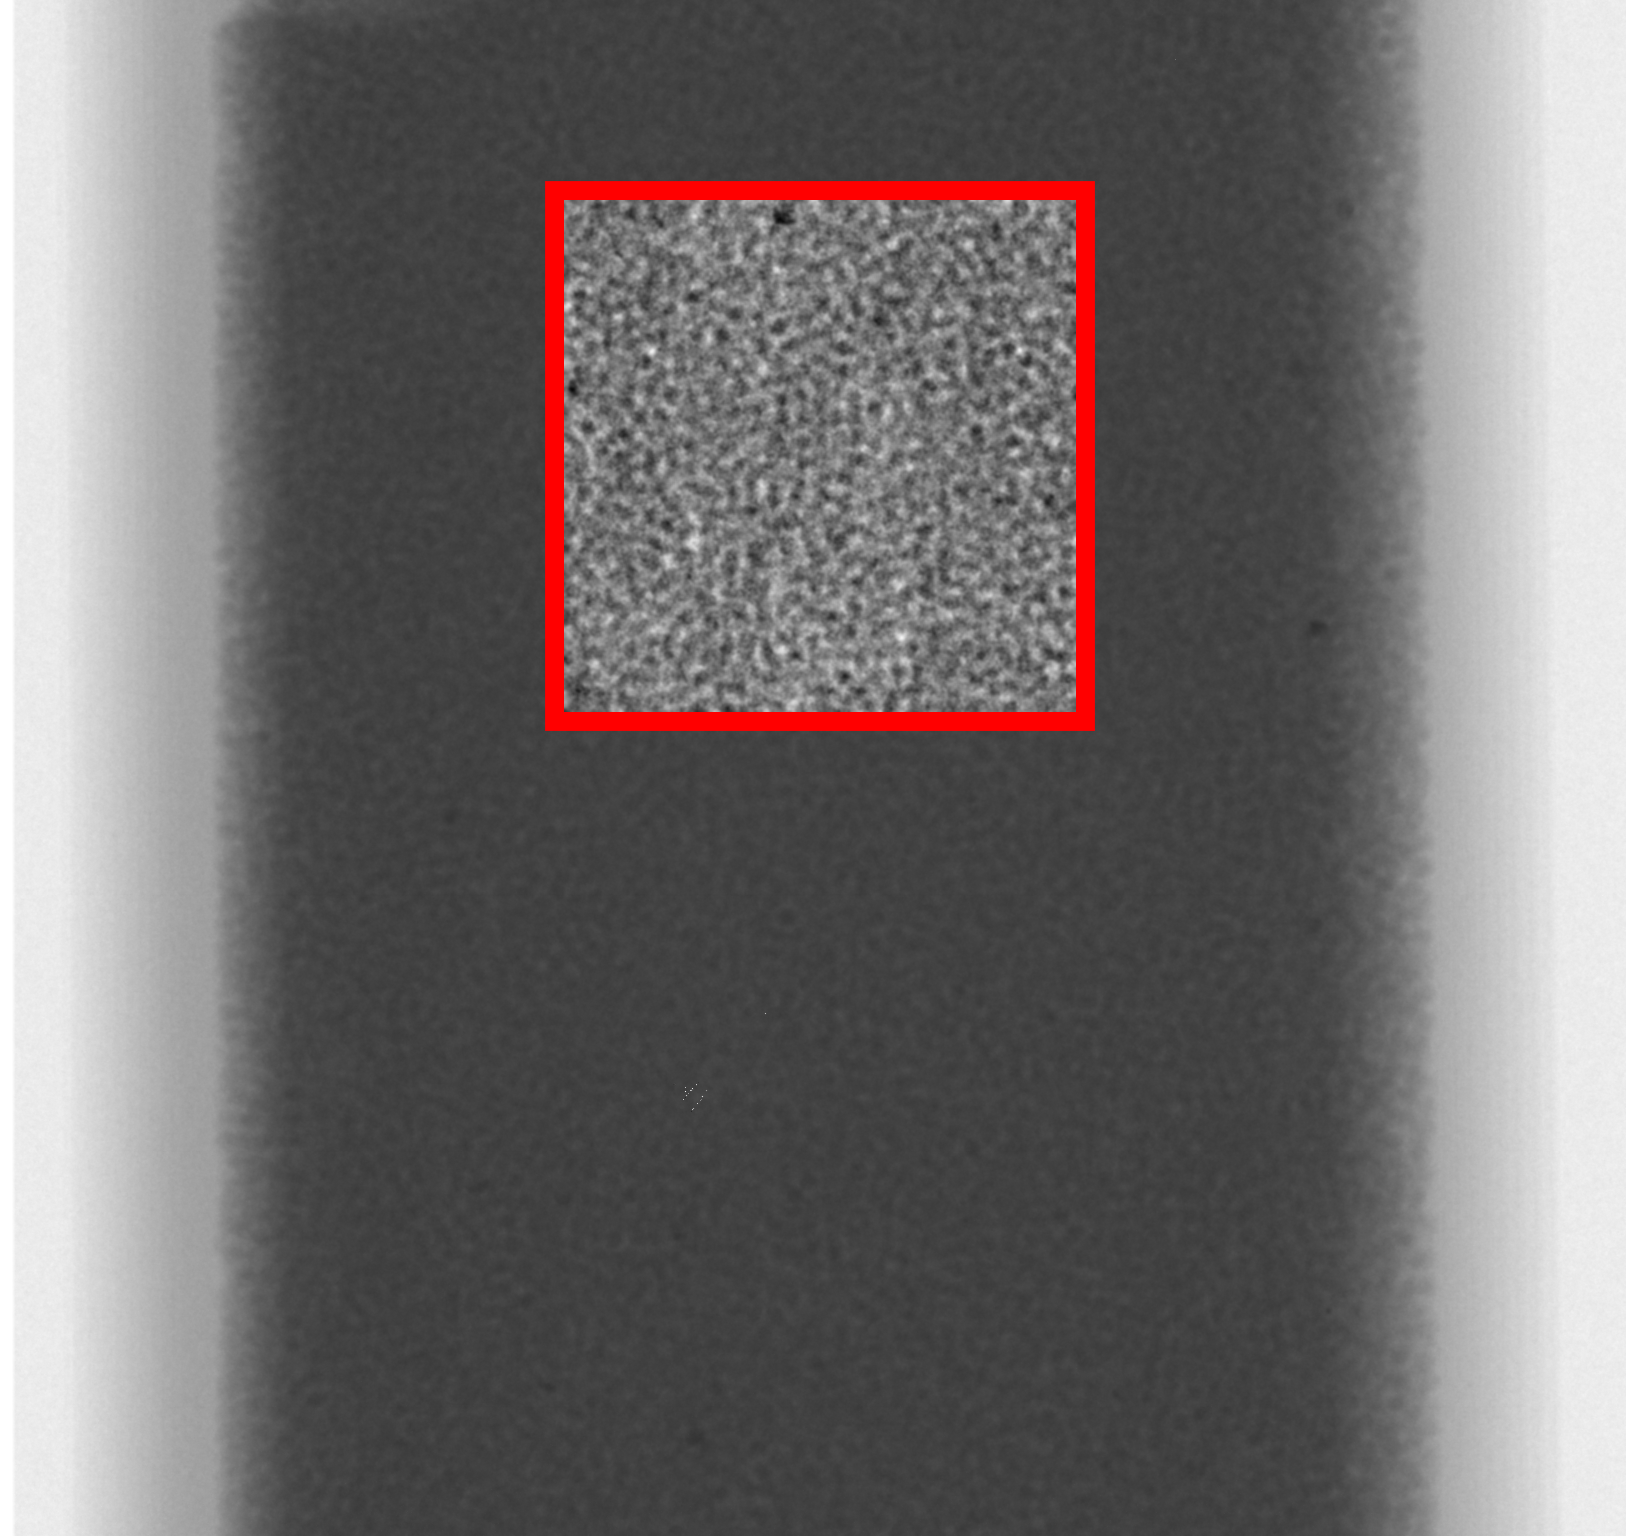
\includegraphics[width=\textwidth]{Sources/X-DFA/radiogram_ROI_marked.png}}
\end{textblock}		

\begin{textblock}{0.3}(0.65,0.6)
	\centering
	\fbox{
	\movie[height=0.7\textwidth, width =0.7\textwidth, poster]
	{
\includegraphics[width=0.7\textwidth]{Sources/X-DFA/cropped_80kV_340uA_38ms_0000.png}}
	{Sources/X-DFA/3500mul_per_min_cropped_roi_512x512.avi}
	}
\end{textblock}
\end{frame}

\frame{
\frametitle{Experiments}

\begin{textblock}{0.6}(0.03,0.1)
	\centering
	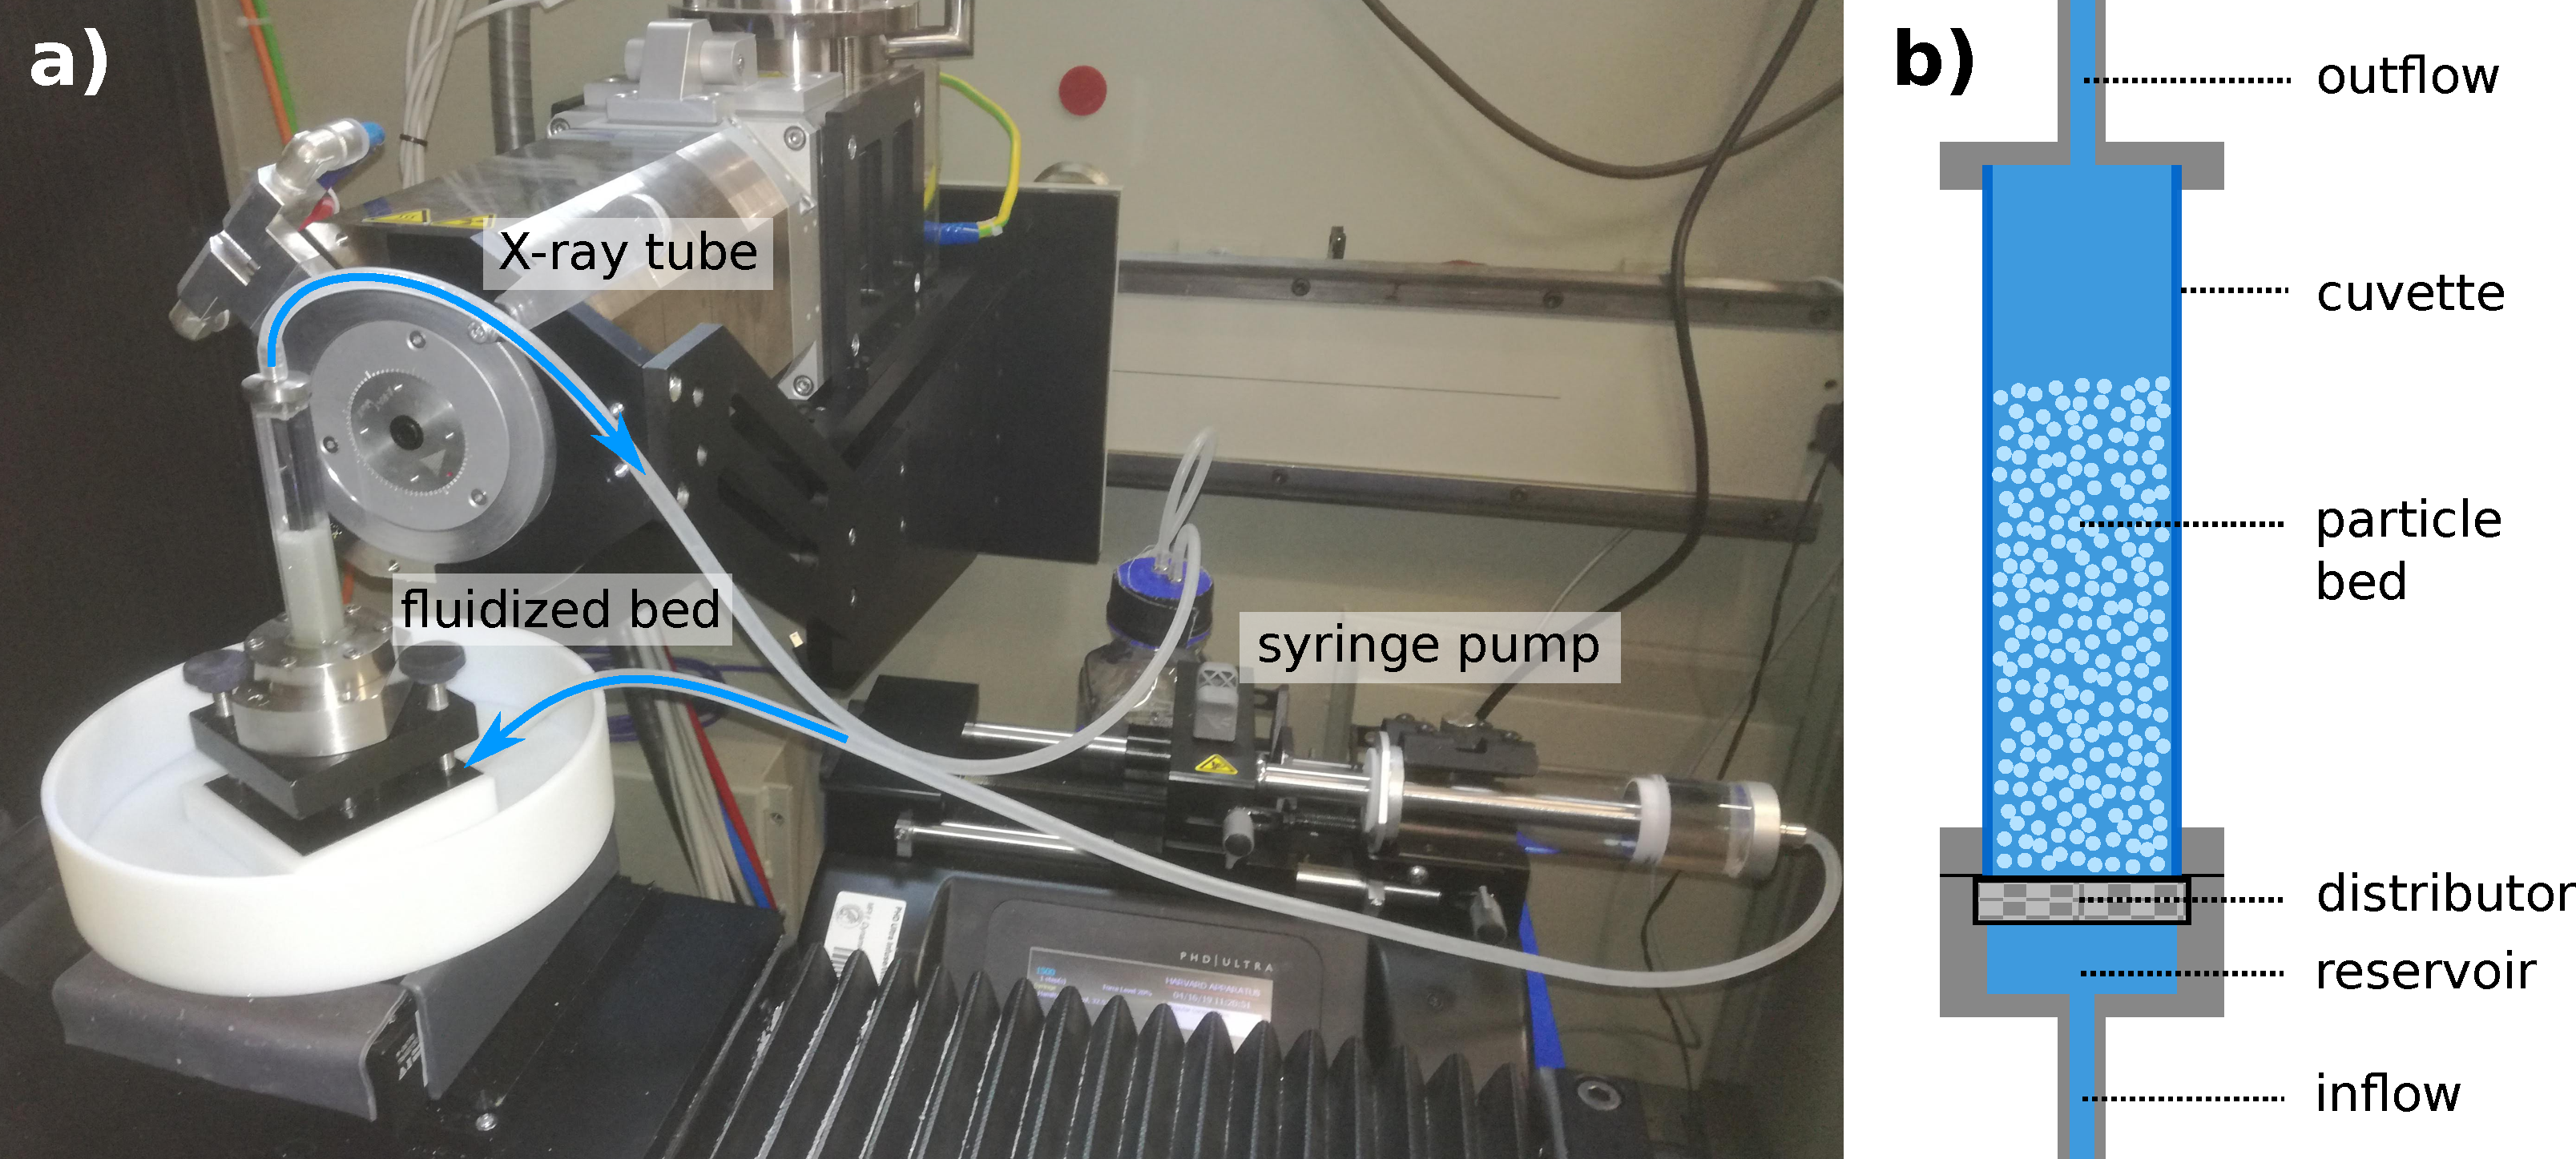
\includegraphics[width=\textwidth]{Sources/X-DFA/setup-photo_and_fluidized_bed_sketch.pdf}
\end{textblock}

\begin{textblock}{0.6}(0.03,0.7)
	\begin{itemize}
		\item volume fraction: $ 0.45 < \Phi < 0.56 $
		\item control dynamics and $\Phi$ via pump rate
	\end{itemize}
\end{textblock}

\begin{textblock}{0.3}(0.67,0.05)
	\centering
		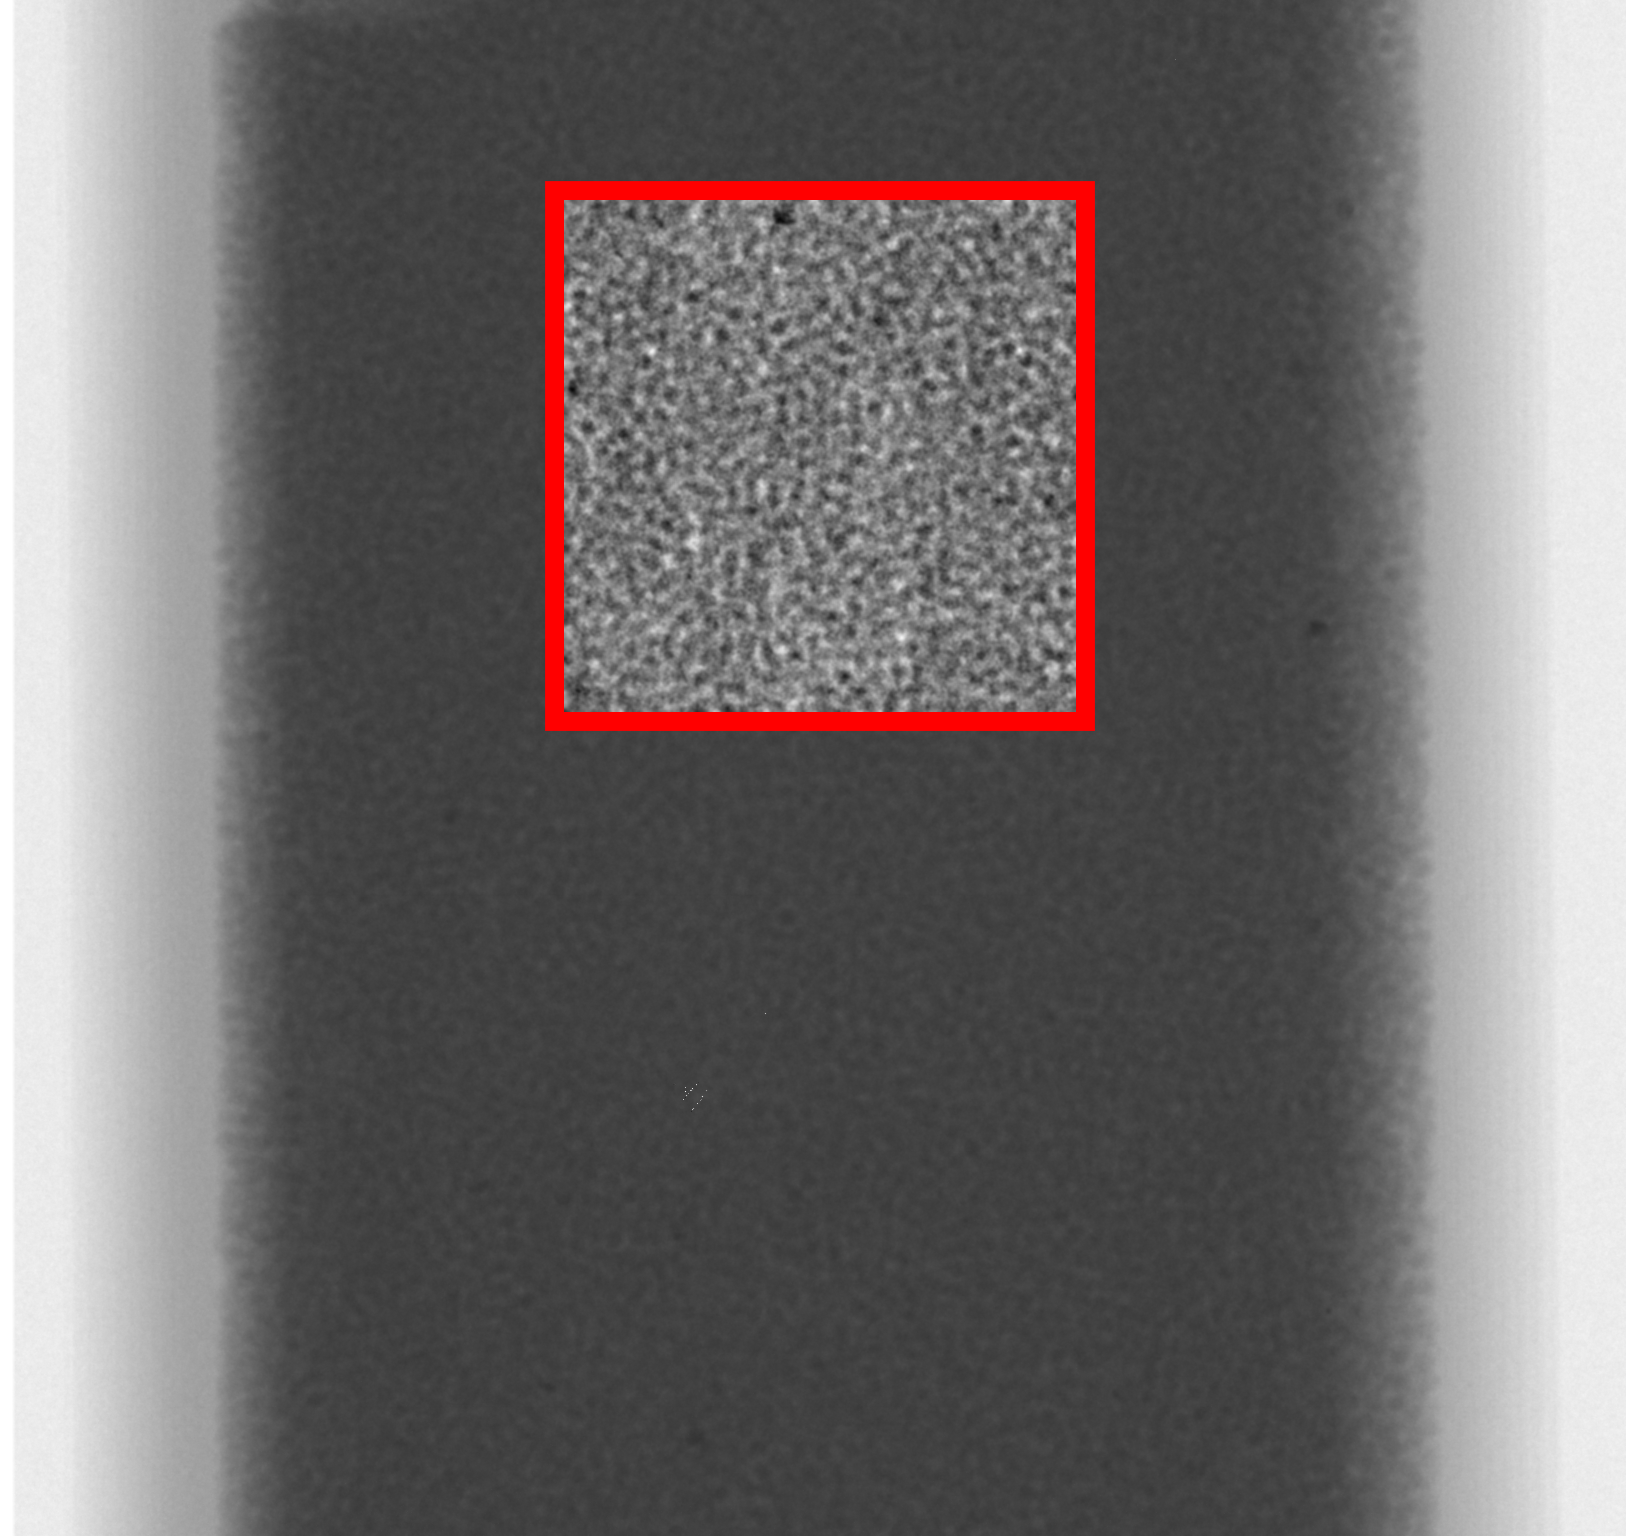
\includegraphics[width=\textwidth]{Sources/X-DFA/radiogram_ROI_marked.png}
\end{textblock}	

\begin{textblock}{0.3}(0.67,0.6)
	\centering
	\movie[height=0.7\textwidth, width =0.7\textwidth, poster]
	{
\includegraphics[width=0.7\textwidth]{Sources/X-DFA/cropped_80kV_340uA_38ms_0000.png}}
	{Sources/X-DFA/3500mul_per_min_cropped_roi_512x512.avi}
\end{textblock}
}


\frame{
	
	\begin{textblock}{0.9}(0.05,0.03)
		\centering
		\visible<2->{
			\Large{\textcolor{red}{
					Extending\\}}}
		\textcolor{blue1}{
			\Large{Differential Dynamic Microscopy (DDM)\\}}
		\visible<2->{
			\Large{\textcolor{red}{
					to X-ray imaging}}}
	\end{textblock}
	
	
	
	\only<1>{
		\begin{textblock}{0.9}(0.05,0.3)
			\centering
			\begin{tabular}{c|c|c}
				\toprule
				& \textbf{up to now} & \textbf{this work}\\
				\hline
				\textbf{system} & dispersion, gels & fluidized bed\\
				\textbf{particles} & colloids & granulate\\
				\textbf{part.\ diameter} & $<1~\upmu\si{m}$ & $\approx 200~\upmu\si{m}$\\
				\textbf{volume fraction } & $\Phi \leq 0.33$ &  $0.45 < \Phi < 0.56$\\
				\textbf{imaging} & light microscope & x-ray radiography\\
				\textbf{dynamics} & 
				\multicolumn{2}{c}{Brownian motion, caging, glassy, collective motion}\\
				\bottomrule
			\end{tabular}
		\end{textblock}
	}	
	
	
	\only<2>{
		\begin{textblock}{0.9}(0.05,0.3)
			\centering
			\begin{tabular}{c|c|c}
				\toprule
				& \textbf{up to now} & \textbf{this work}\\
				\hline
				\textbf{system} & dispersion, gels & fluidized bed\\
				\textbf{particles} & colloids & \textcolor{red}{granulate}\\
				\textbf{part.\ diameter} & $<1~\upmu\si{m}$ & $\approx 200~\upmu\si{m}$\\
				\textbf{volume fraction } & $\Phi \leq 0.33$ &  $0.45 < \Phi < 0.56$\\
				\textbf{imaging} & light microscope & \textcolor{red}{x-ray radiography}\\
				\textbf{dynamics} & 
				\multicolumn{2}{c}{Brownian motion, caging, glassy, collective motion}\\
				\bottomrule
			\end{tabular}
		\end{textblock}
	}	
	
	
	\begin{textblock}{0.9}(0.05,0.8)
		\centering
		\visible<2->{
			\Large{\textcolor{red}{
					Digital Fourier Analysis of X-Ray Radiograms (X-DFA)}}}
	\end{textblock}
	
	\begin{textblock}{0.7}(0.05,0.95)
		\footnotesize{Giavazzi \textit{et al}, PRE \textbf{80}, 031403 (2009)}
	\end{textblock}
	
}



\frame{
\frametitle{Synthetic radiograms}
	
\begin{textblock}{0.4}(0.05,0.2)
	\centering
	\fbox{
	\movie[width =0.8\textwidth, poster, loop]
	{
\includegraphics[width=0.8\textwidth]{Sources/X-DFA/fake_img_nPart10.png}}
	{Sources/X-DFA/10_particles.avi}}
\end{textblock}
%\begin{textblock}{0.4}(0.05,0.2)
%	\centering
%	\fbox{
\includegraphics[width=0.8\textwidth]{Sources/X-DFA/fake_img_nPart10.png}}\\
%	\vspace{0.5cm}
%	\href{run:Sources/X-DFA/10_particles.avi}{\textcolor{red}{Video 10 Particles}}
%%	\includemedia[
%%	label=some_dice,
%%	width=0.8\textwidth,height=0.8\textwidth, % 16:9
%%	addresource=Sources/X-DFA/10_particles.avi, 
%%	transparent,
%%	activate=pageopen,
%%	passcontext,
%%	flashvars={
%%		source=Sources/X-DFA/10_particles.avi
%%		&autoPlay=false % start playing on activation
%%		&loop=true
%%	}
%%	]{}{VPlayer.swf}
%\end{textblock}

\begin{textblock}{0.45}(0.55,0.2)
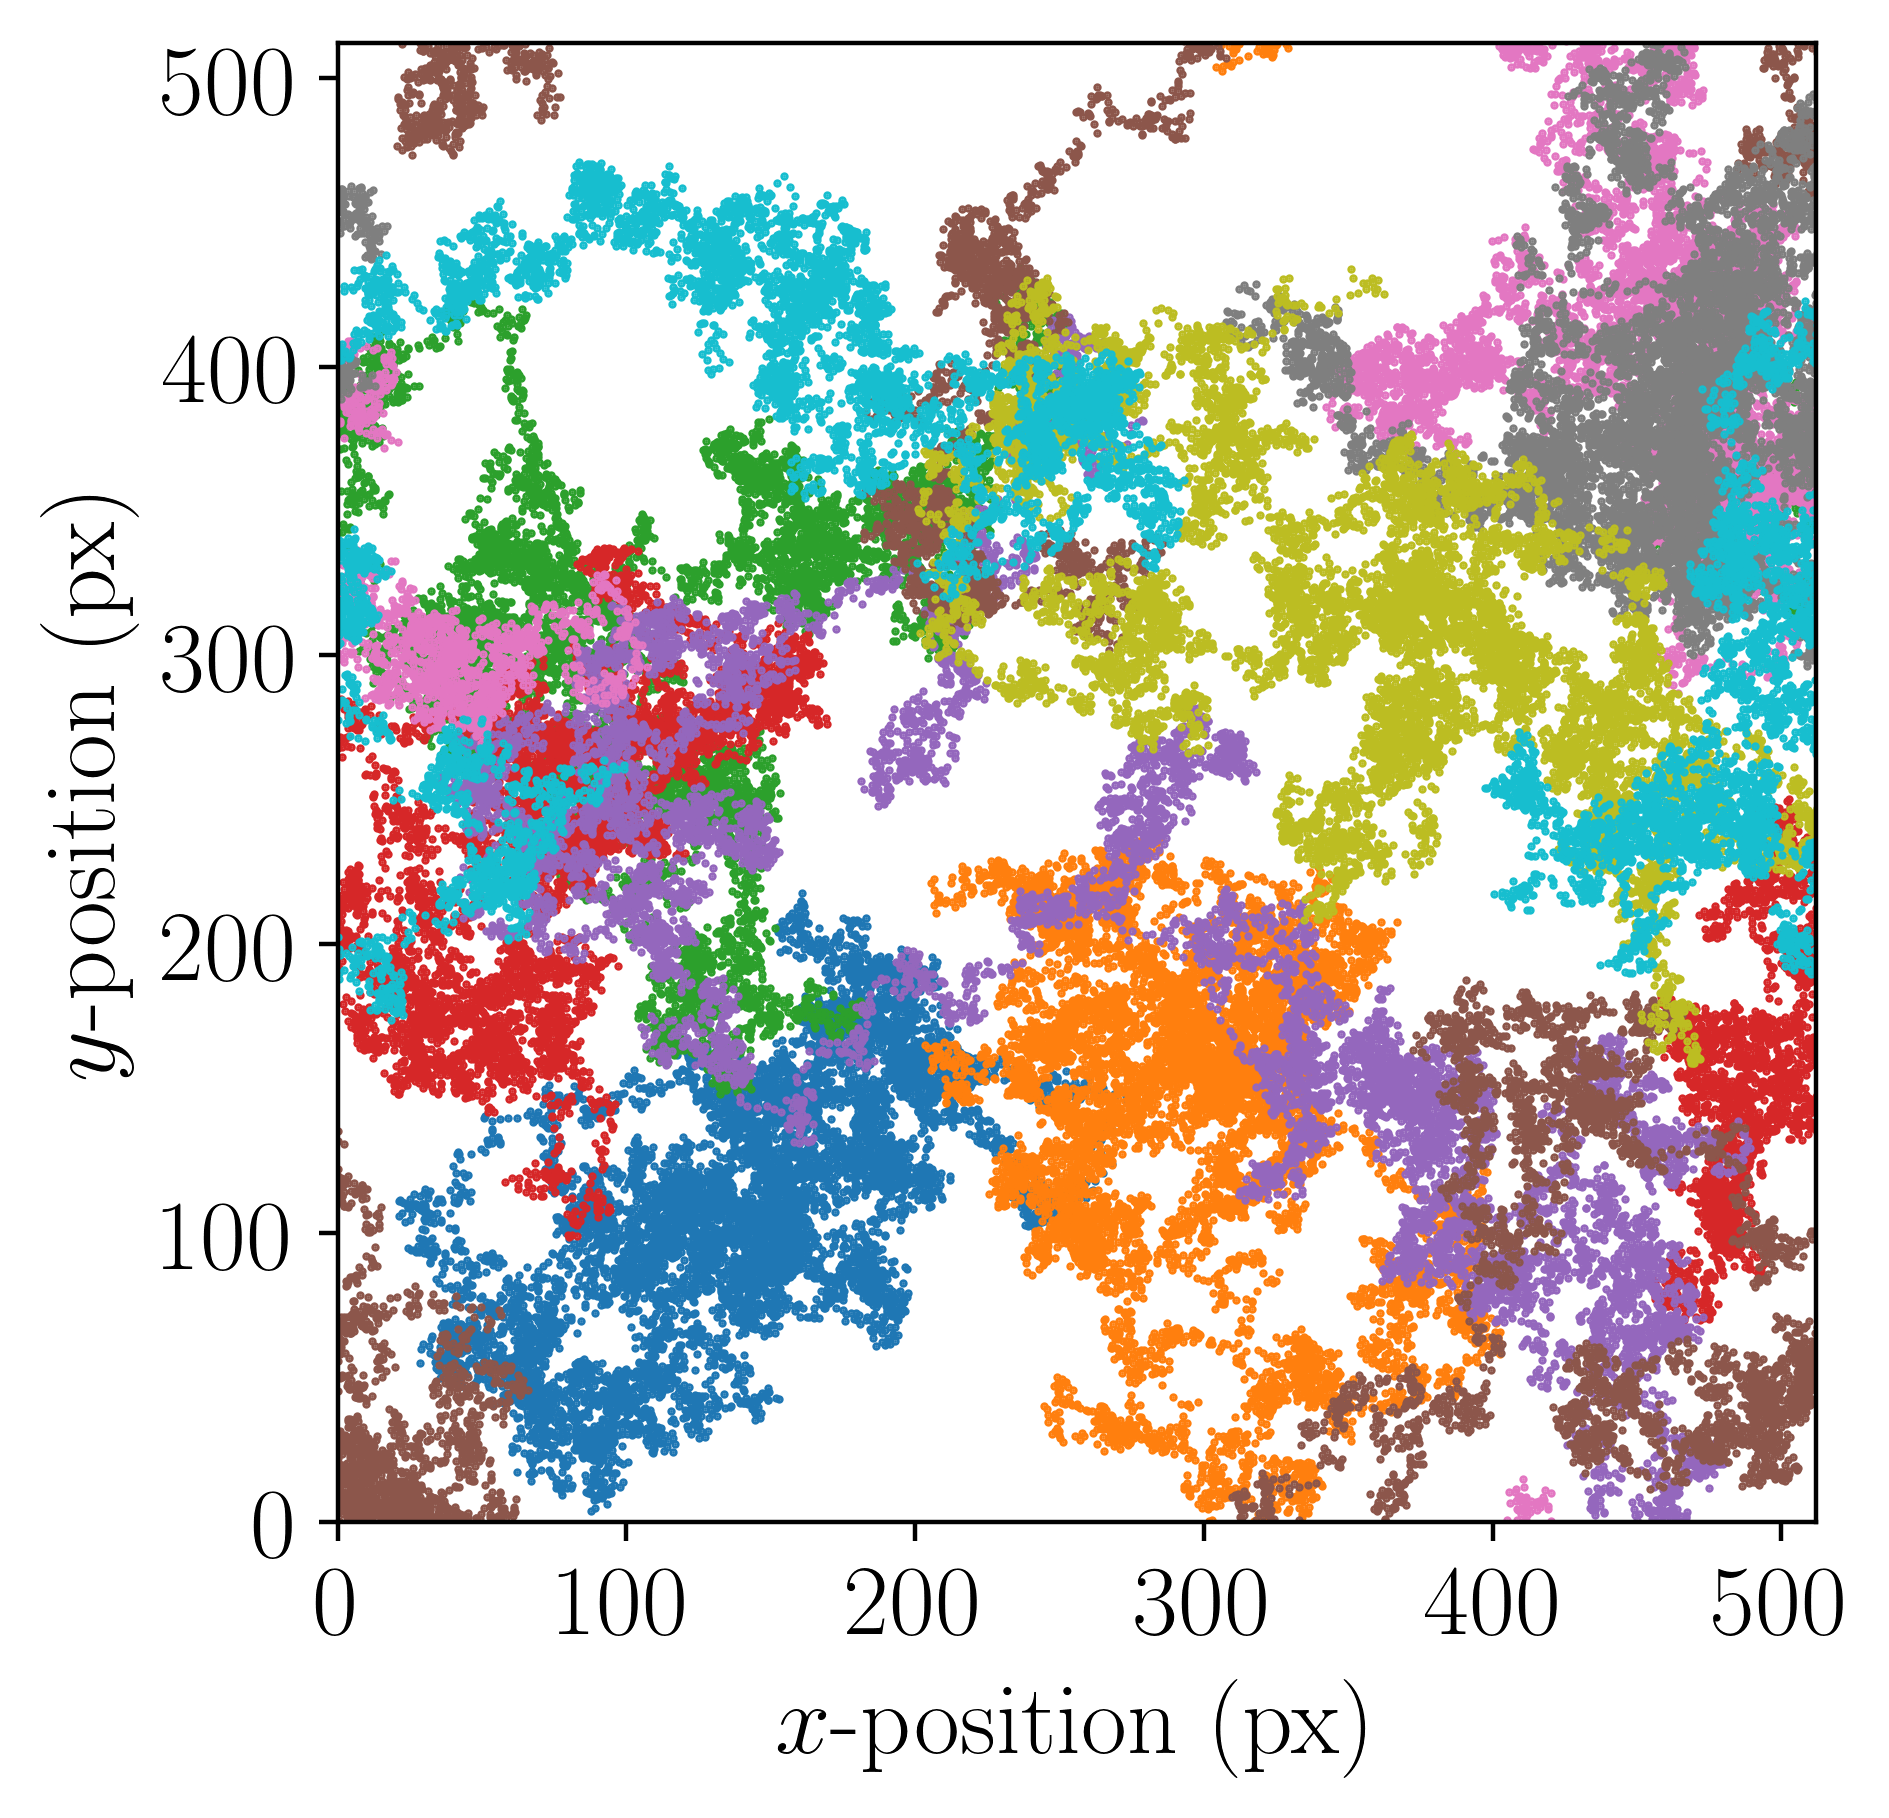
\includegraphics[width=0.8\textwidth]{Sources/X-DFA/trajectory_plot_nPart10.png}
\end{textblock}
}


\frame{
	\frametitle{Synthetic radiograms}
	
	\begin{textblock}{0.9}(0.03,0.05)
		\centering
		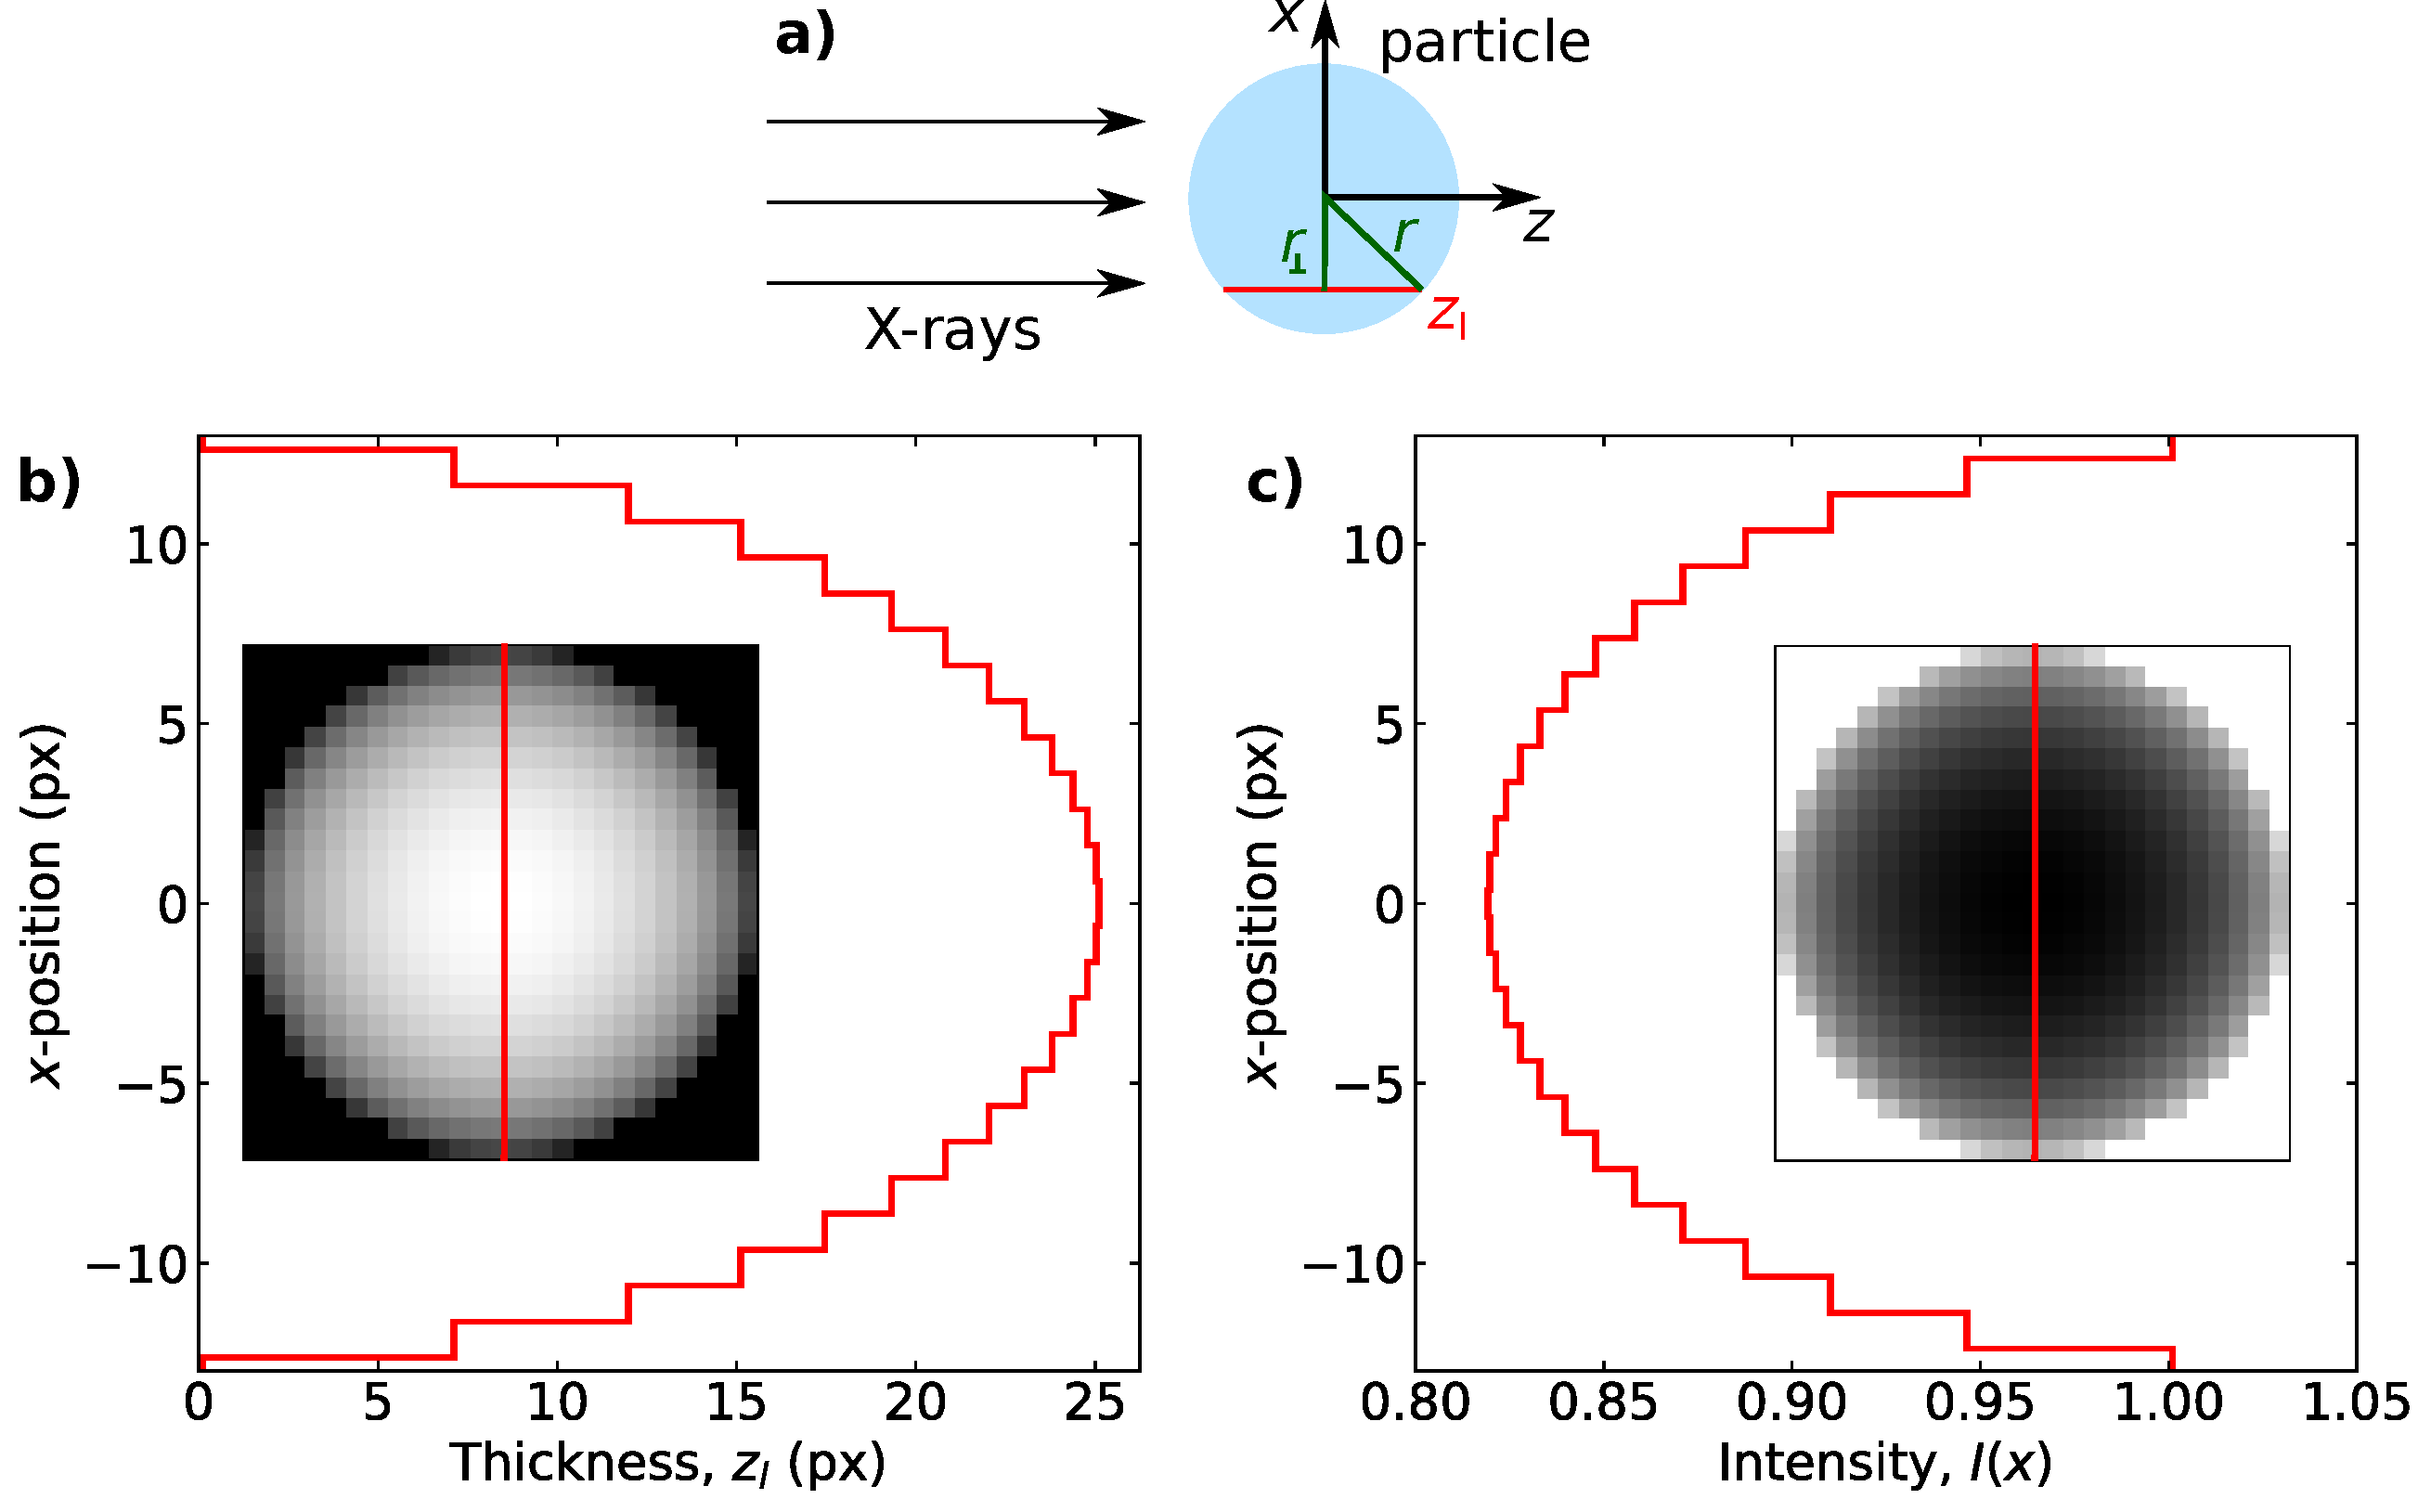
\includegraphics[width=0.6\textwidth]{Sources/X-DFA/particle_mask_construction.pdf}
	\end{textblock}

	\begin{textblock}{0.9}(0.05,0.8)
	\centering
	Beer-Lambert\\
	$I(z_l) = I_0 \exp(-\mu z)$
	\end{textblock}

	\begin{textblock}{0.2}(0.03,0.6)
		\visible<2->{
		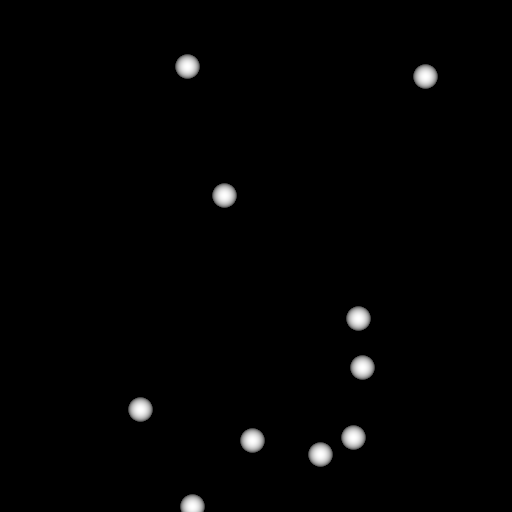
\includegraphics[width=\textwidth]{Sources/X-DFA/thicknessMap_nPart10.png}}
	\end{textblock}

	\begin{textblock}{0.2}(0.77,0.6)
	\visible<2->{
	\frame{
	
\includegraphics[width=\textwidth]{Sources/X-DFA/fake_img_nPart10.png}
	}}
	\end{textblock}
}





\frame{
	\frametitle{The image structure function $D(\mathbf{q}, \tau)$}
	\begin{textblock}{0.9}(0.05,0.1)
		\centering
		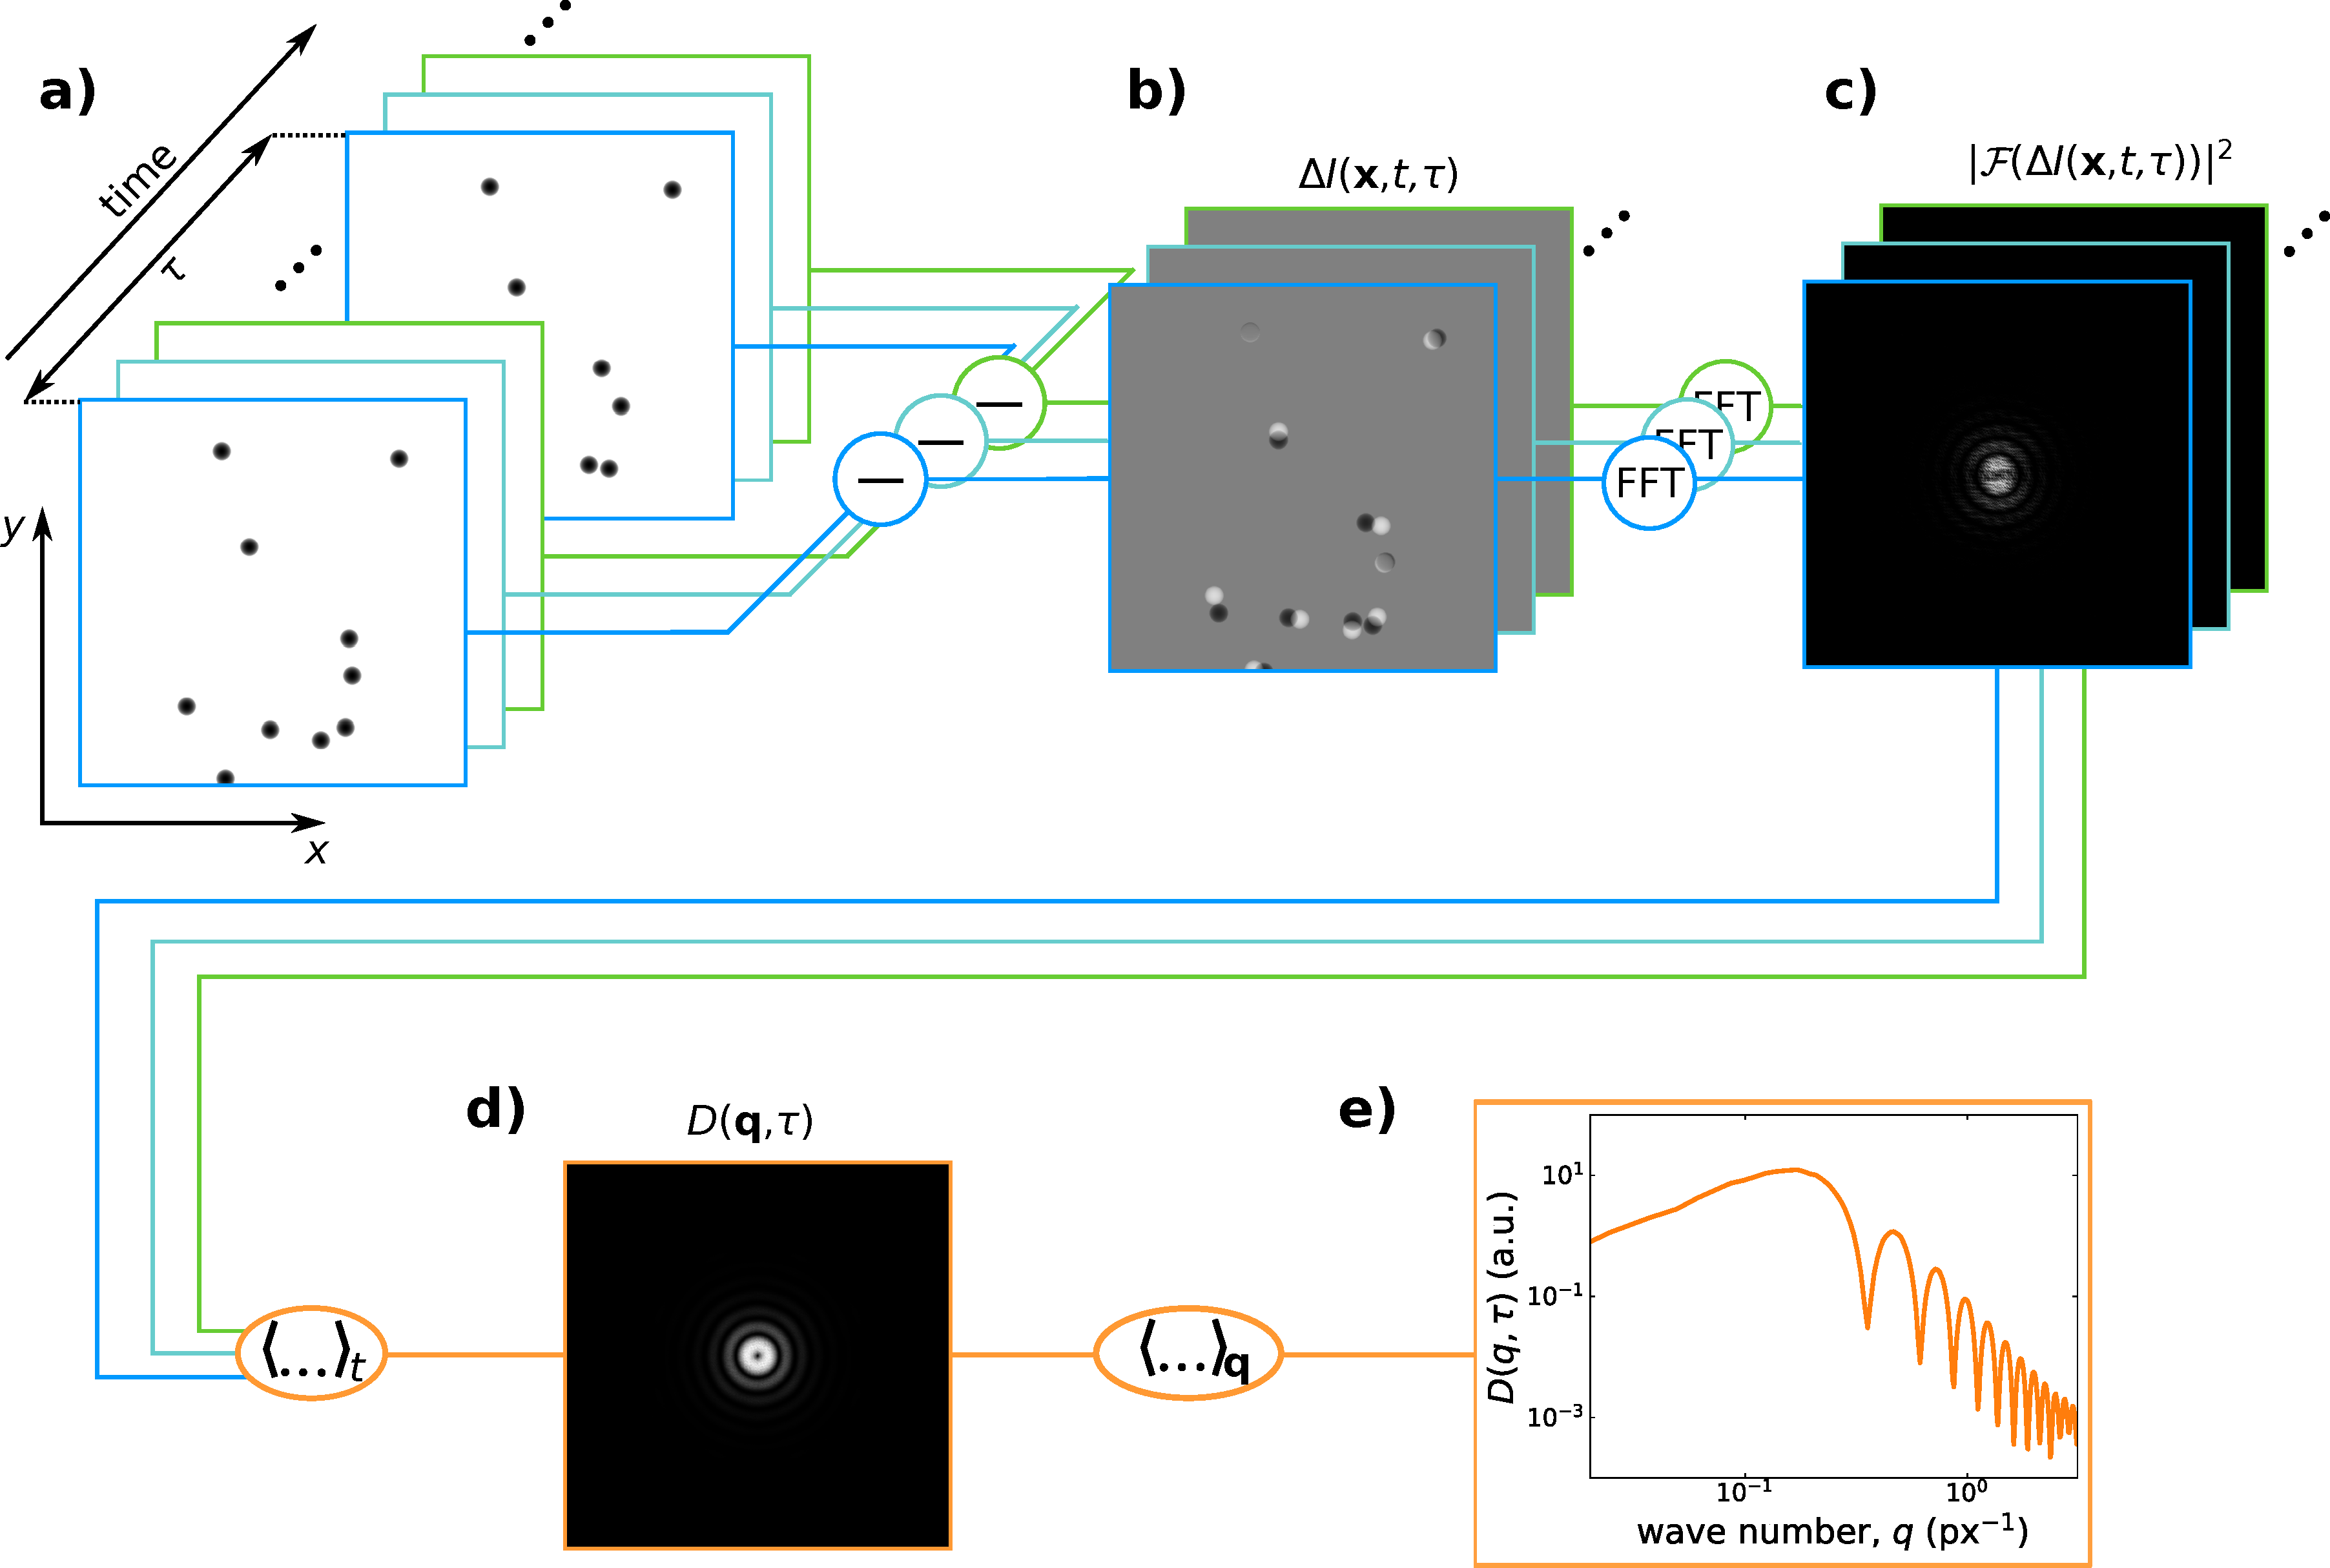
\includegraphics[width=0.8\textwidth]{Sources/X-DFA/image_structure_function.pdf}
	\end{textblock}

	\begin{textblock}{0.7}(0.02,0.95)
		\scriptsize{Giavazzi \textit{et al}, PRE \textbf{80}, 031403 (2009)}
	\end{textblock}
}



%%%%%%%%%%%%%%%%%%%%%%%%%%%%%%%%%%%%%%%%%%%%%%%%%%%%%%%%%%%%%%%%%%%%%%%%%%%%%%%%%%%%%%%%%%%%%%%
%%%%%%% Build the image structure function for every time step
\frame{
	\frametitle{The image structure function $D(q,\tau)$}

	\begin{textblock}{0.3}(0.05,0.1)
	\only<1>{
	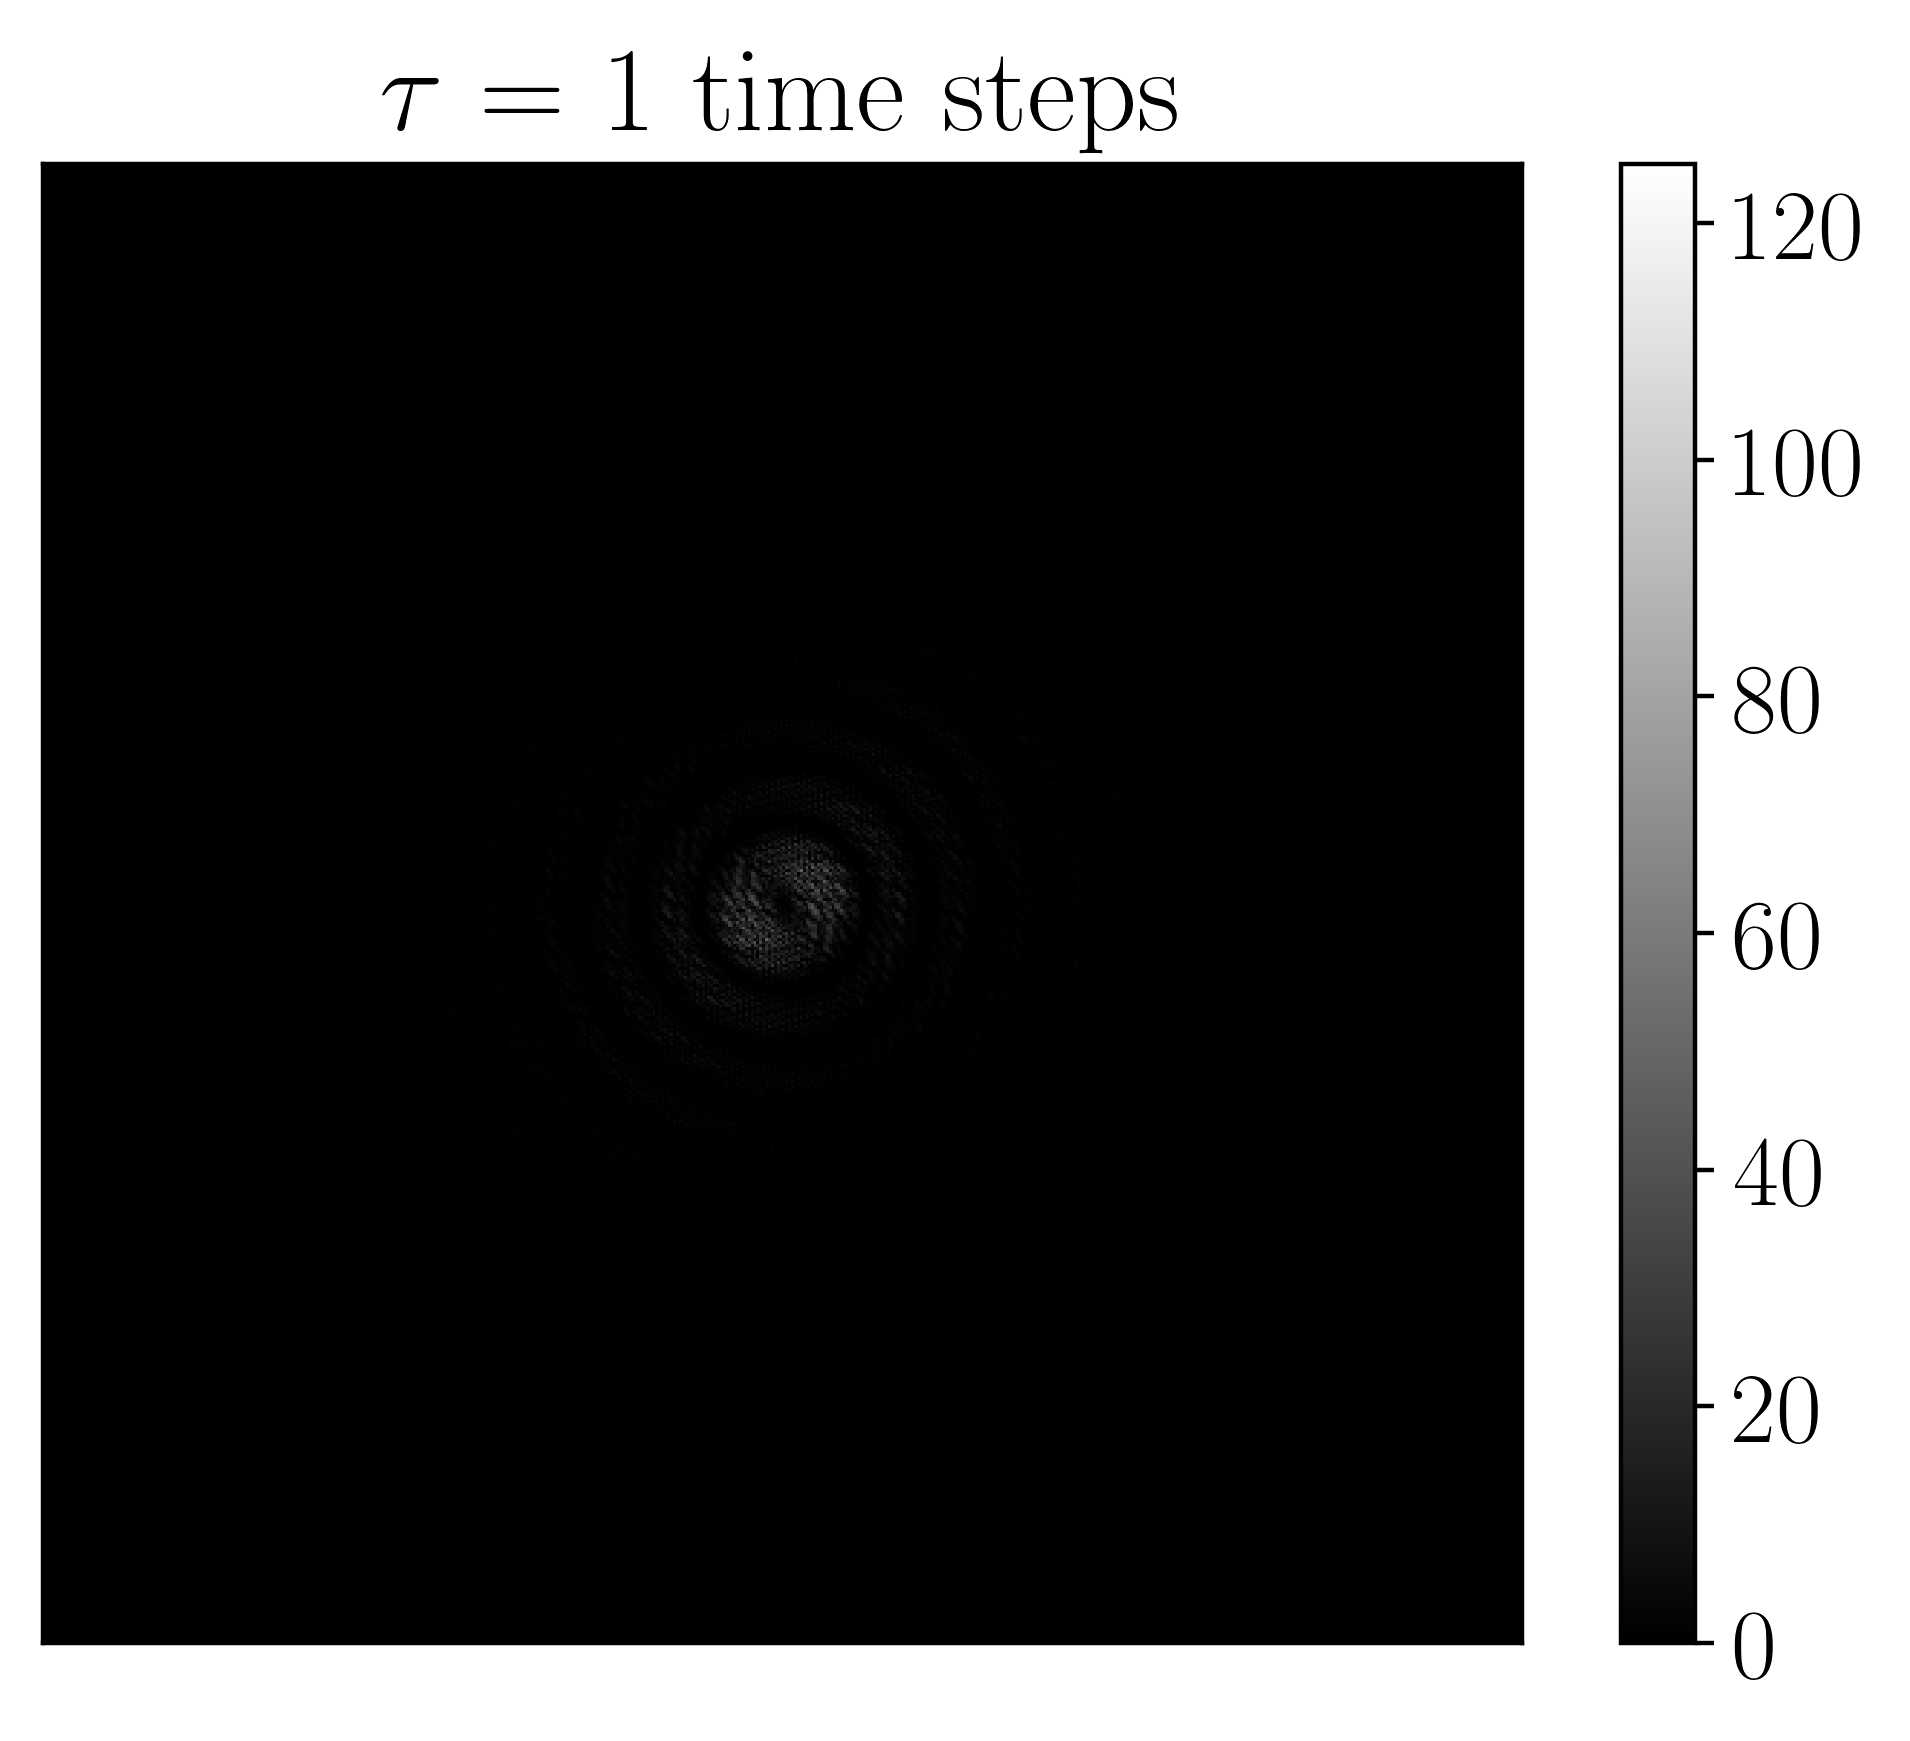
\includegraphics[width=\textwidth]
	{Sources/X-DFA/Mag_Spectrum_d_img_00000.png}}

	\only<2>{
	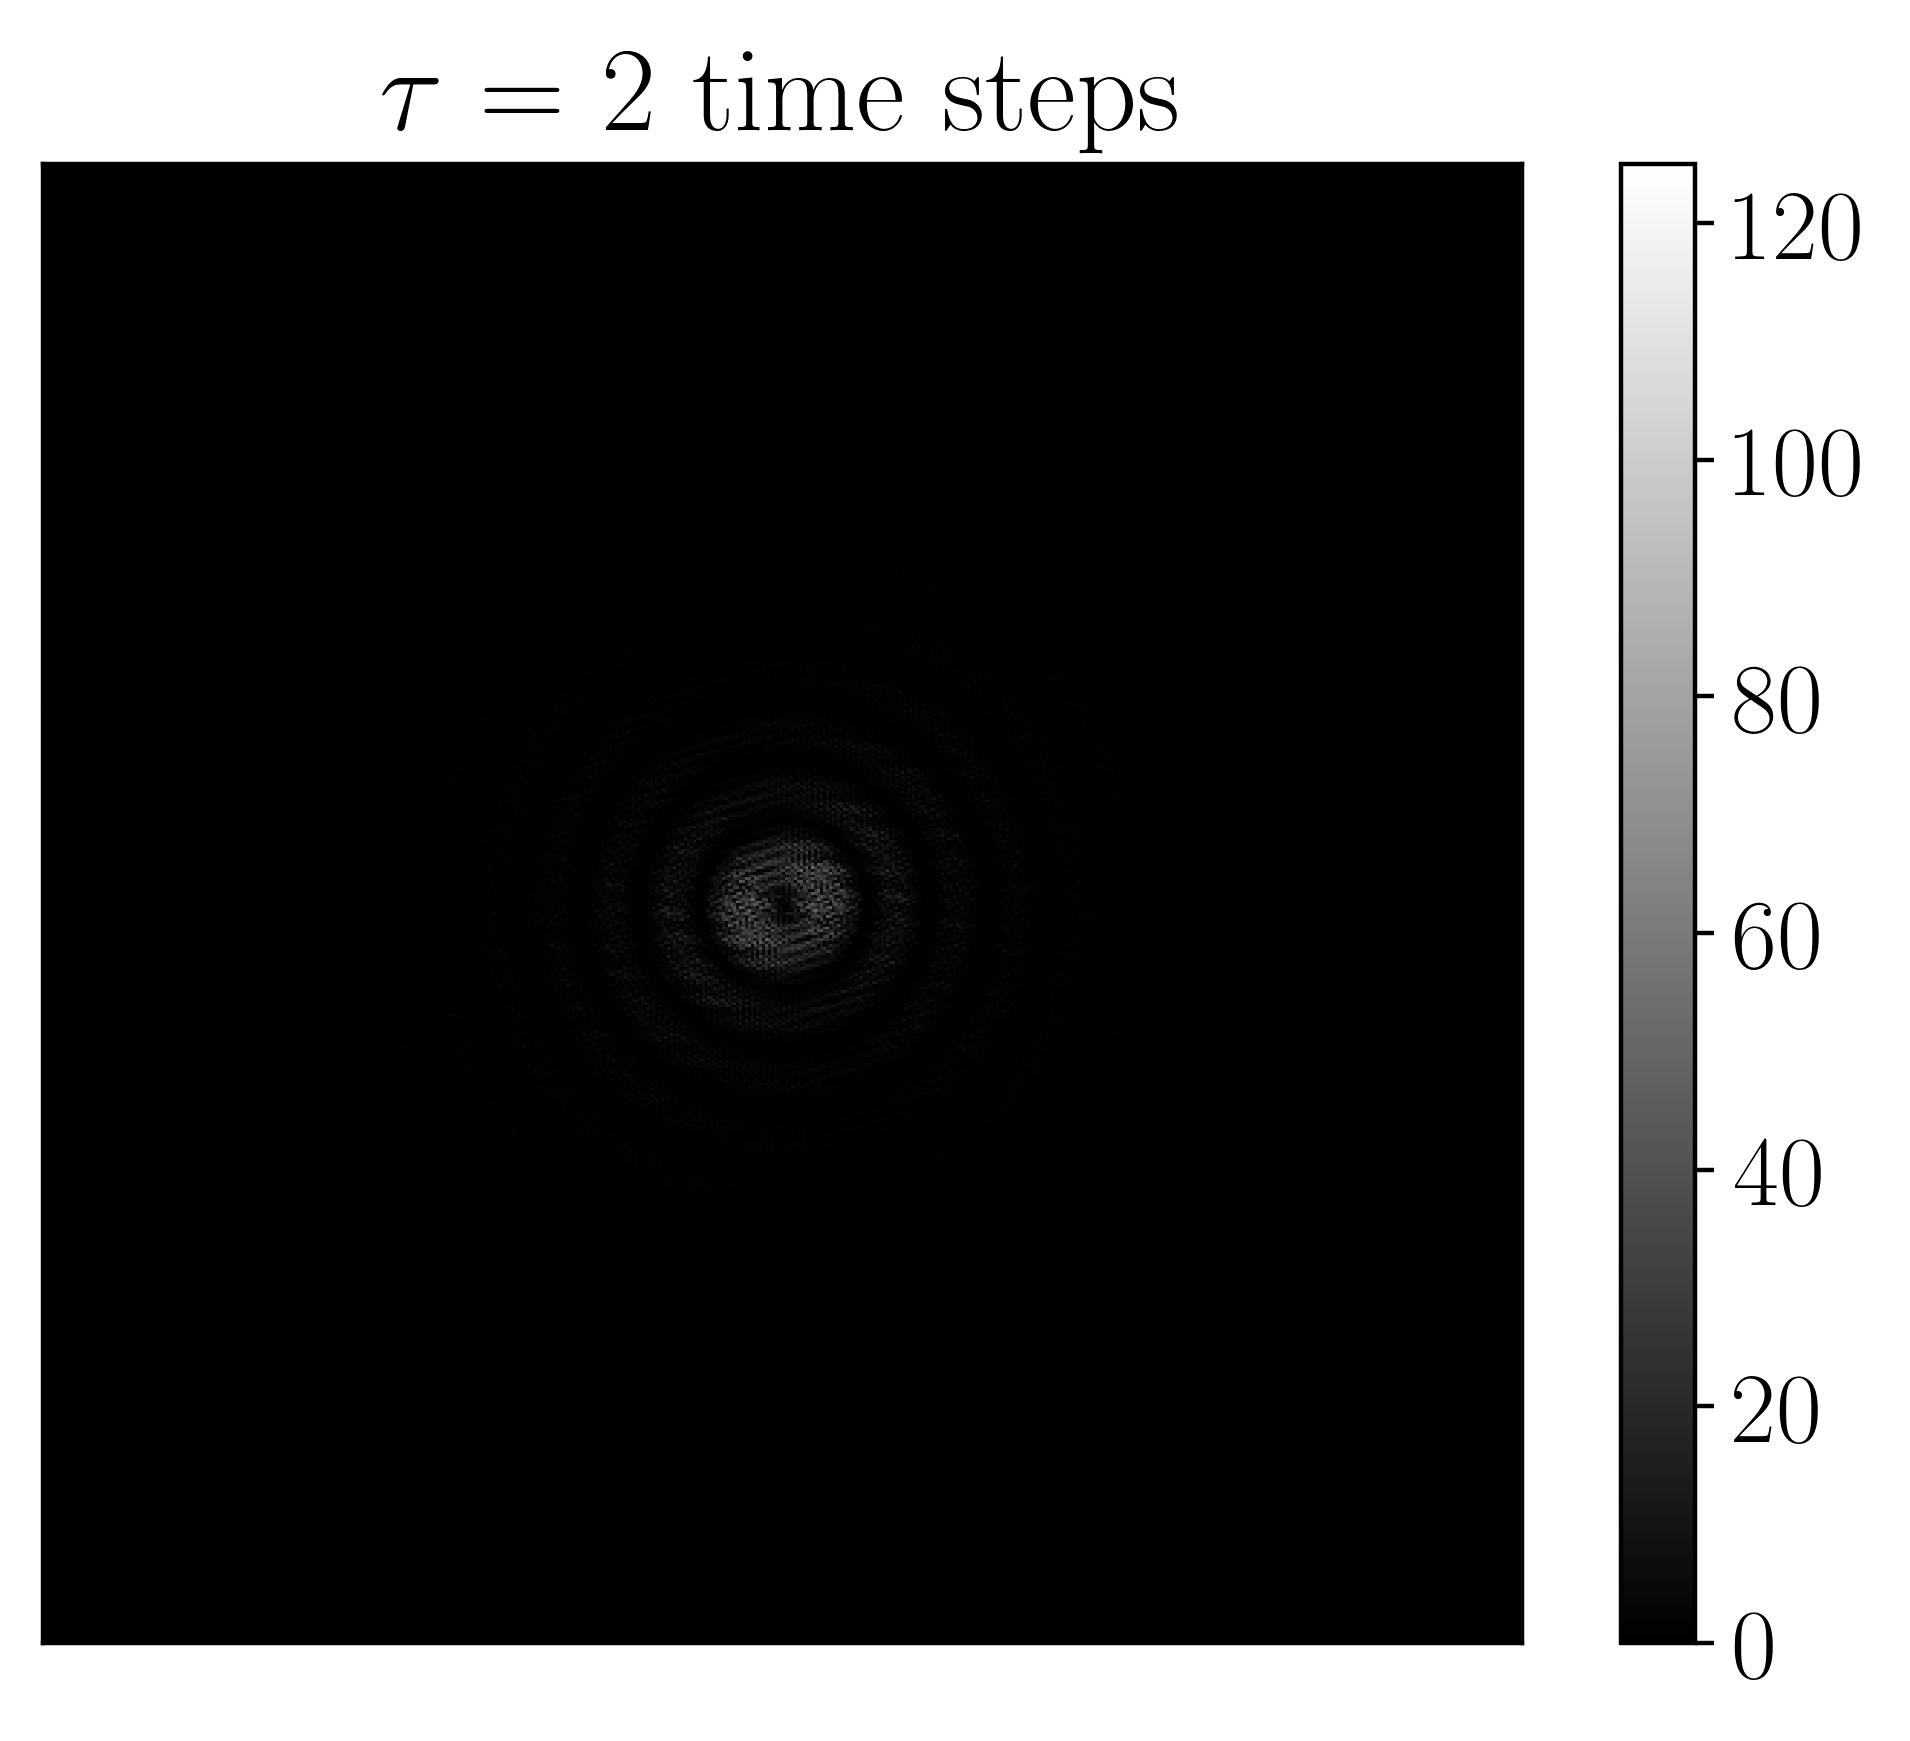
\includegraphics[width=\textwidth]
	{Sources/X-DFA/Mag_Spectrum_d_img_00001.png}}

	\only<3>{
	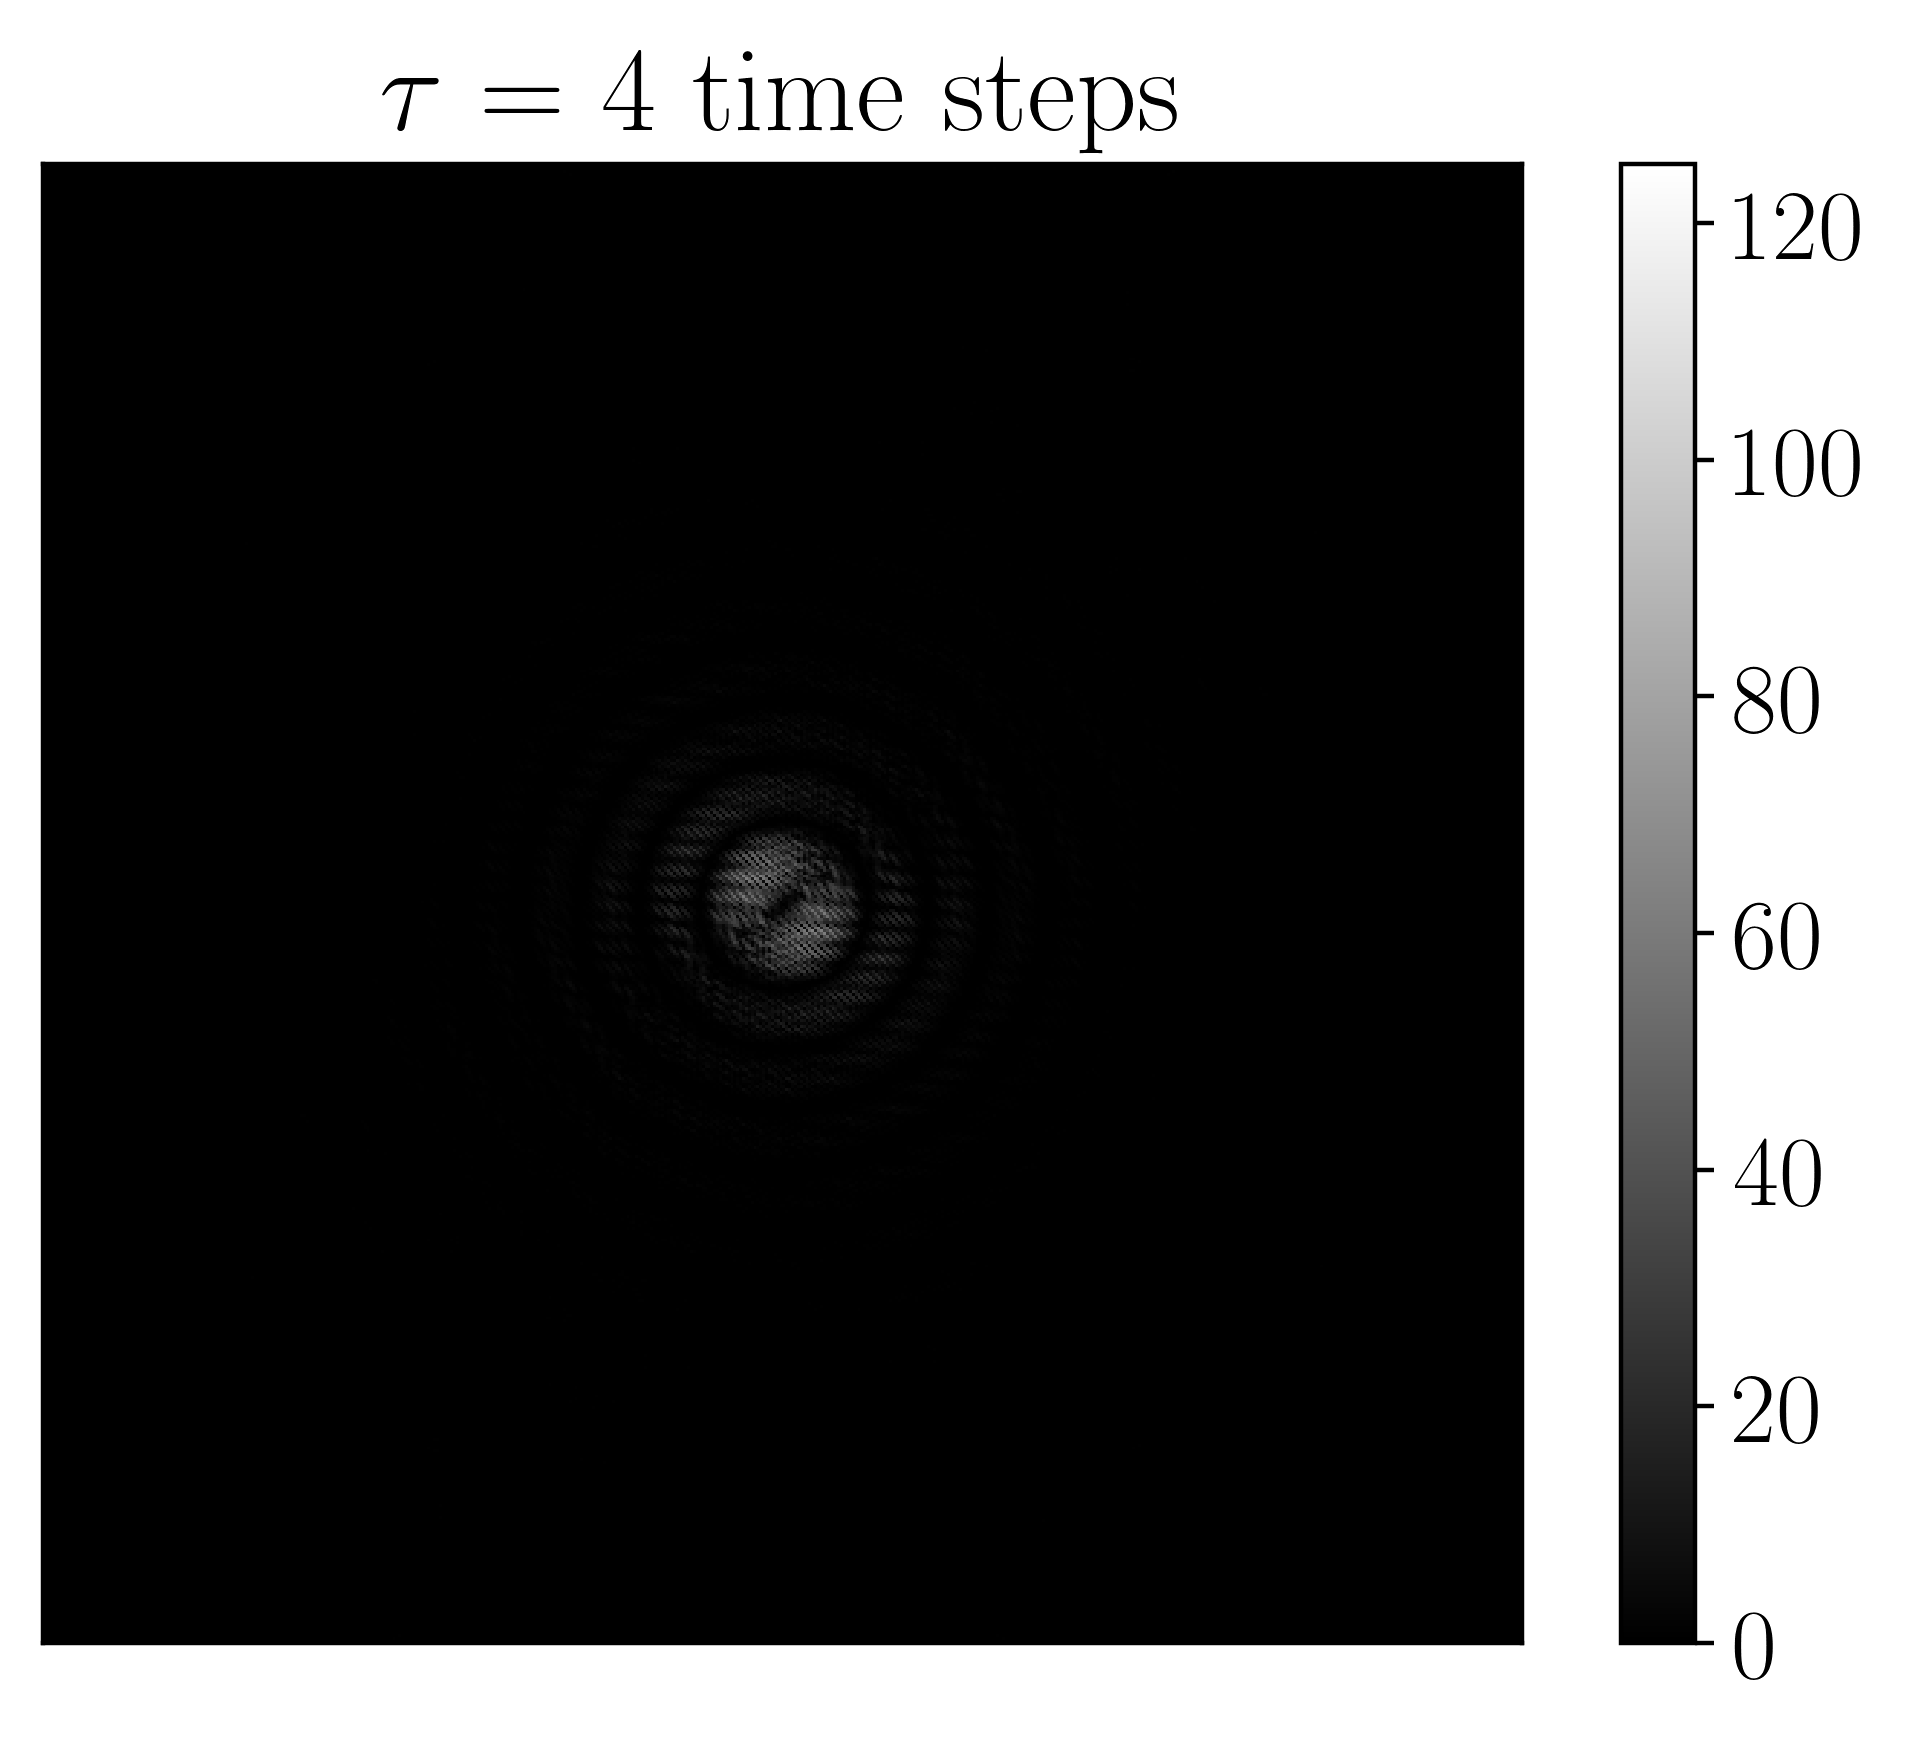
\includegraphics[width=\textwidth]
	{Sources/X-DFA/Mag_Spectrum_d_img_00003.png}}

	\only<4>{
	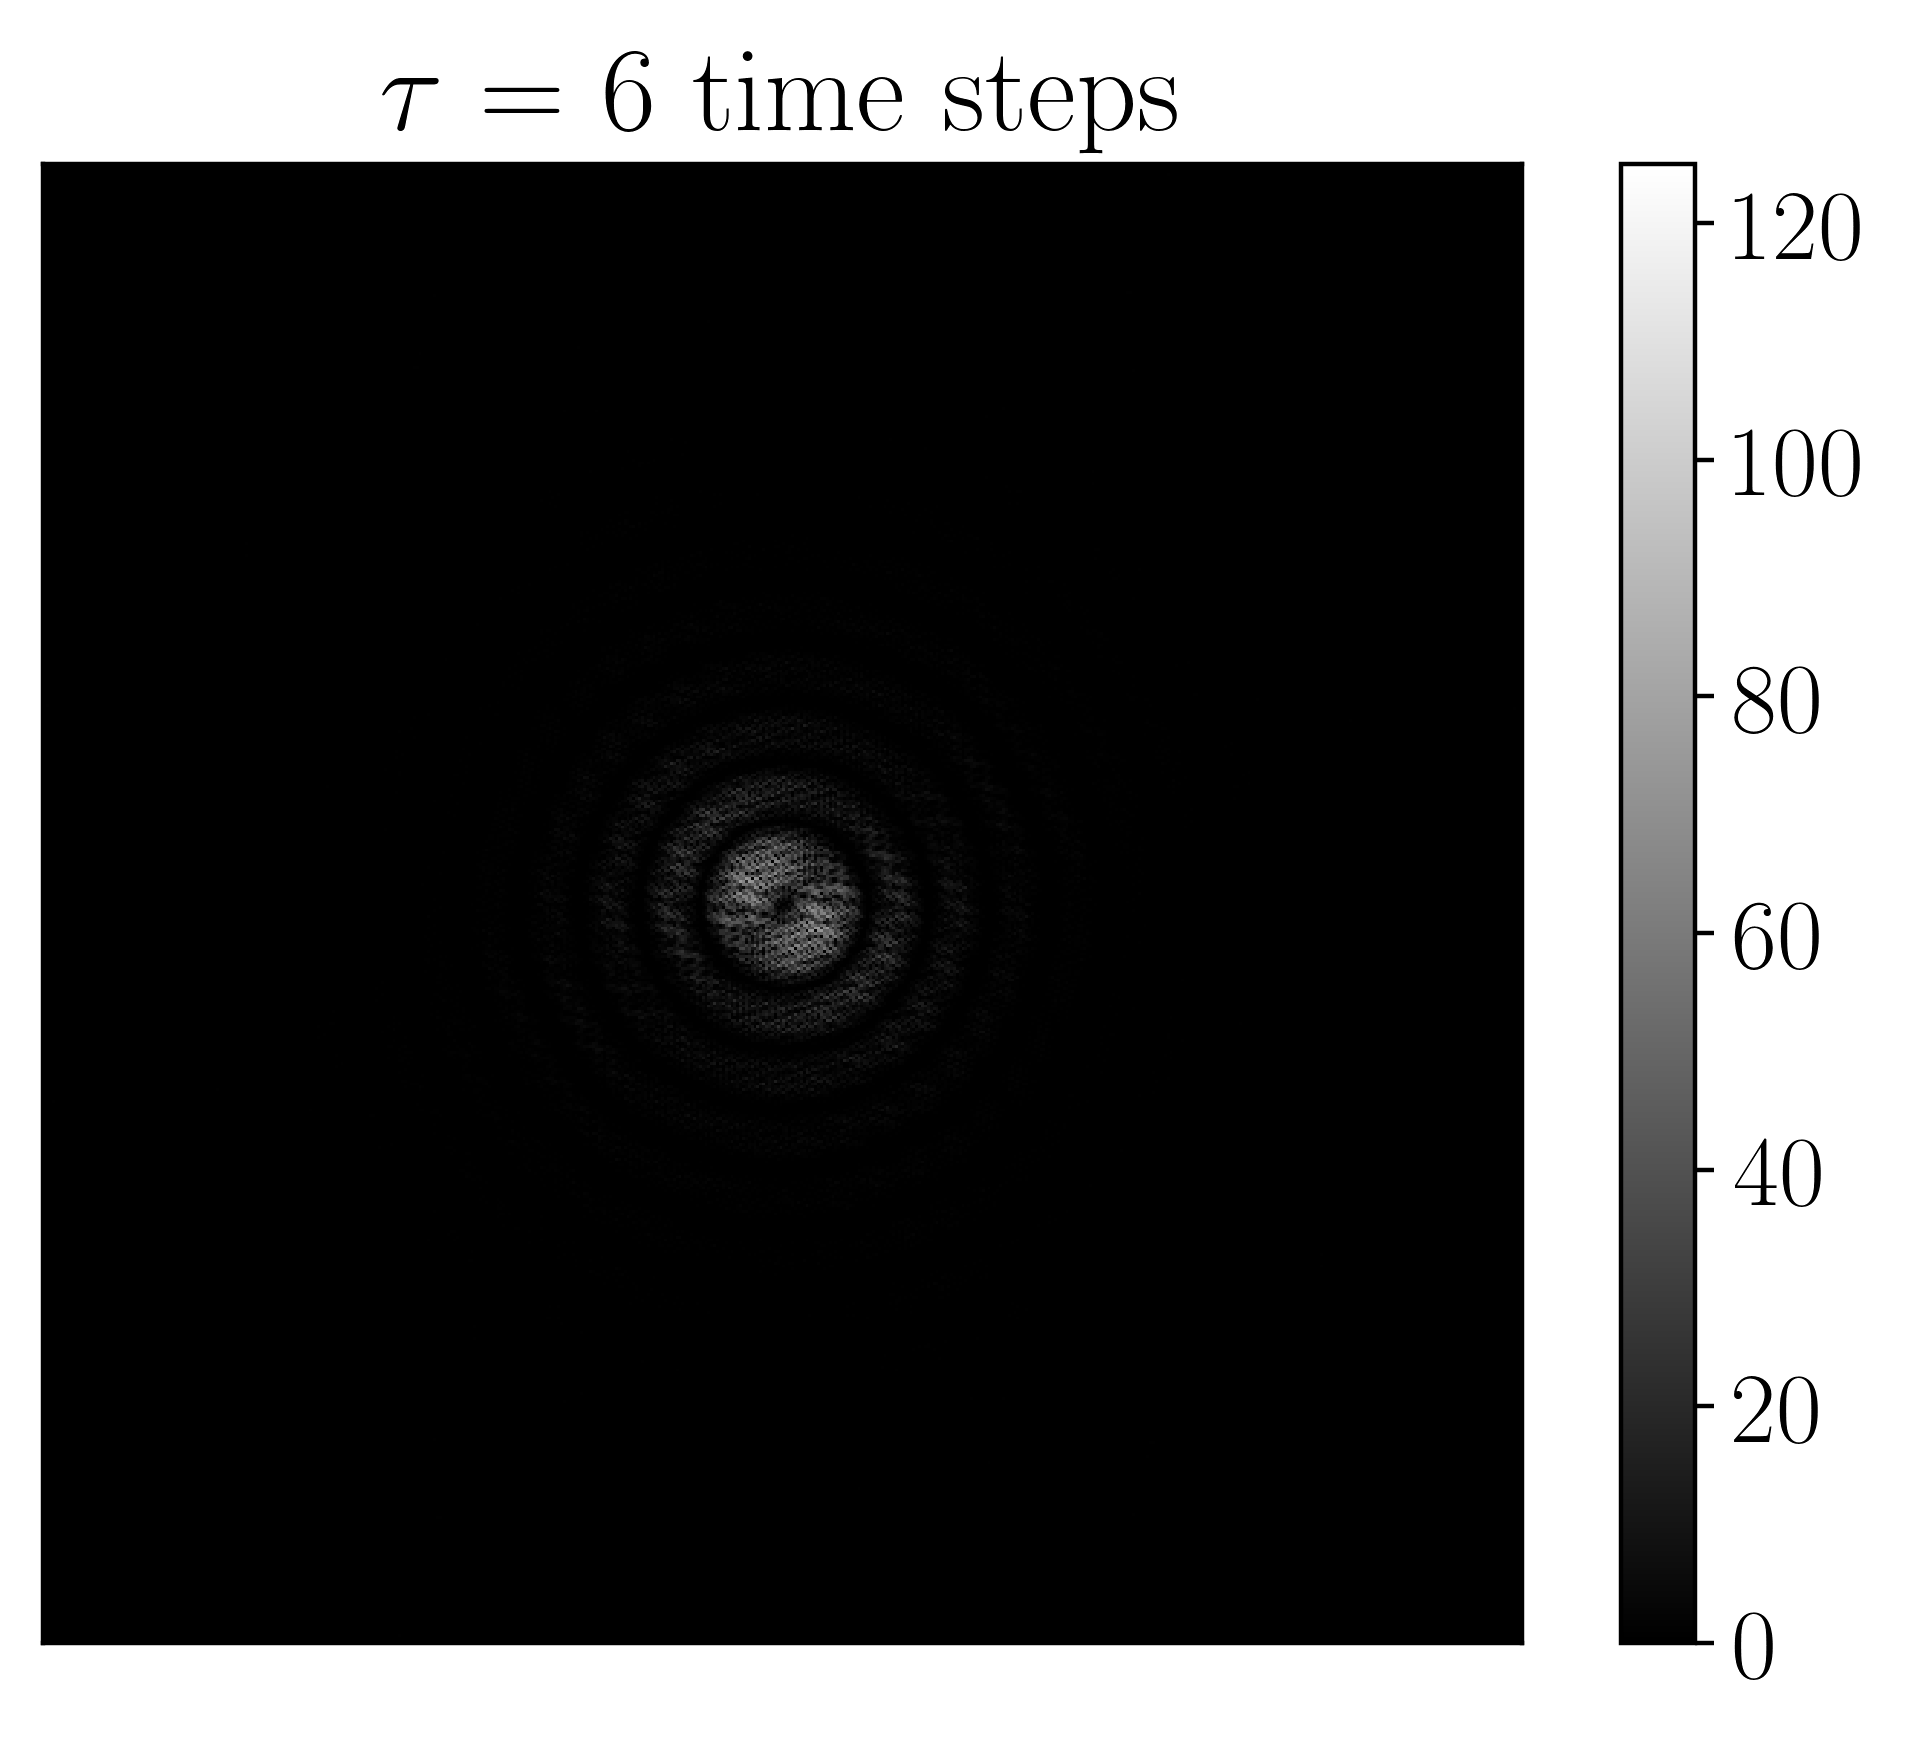
\includegraphics[width=\textwidth]
	{Sources/X-DFA/Mag_Spectrum_d_img_00005.png}}

	\only<5>{
	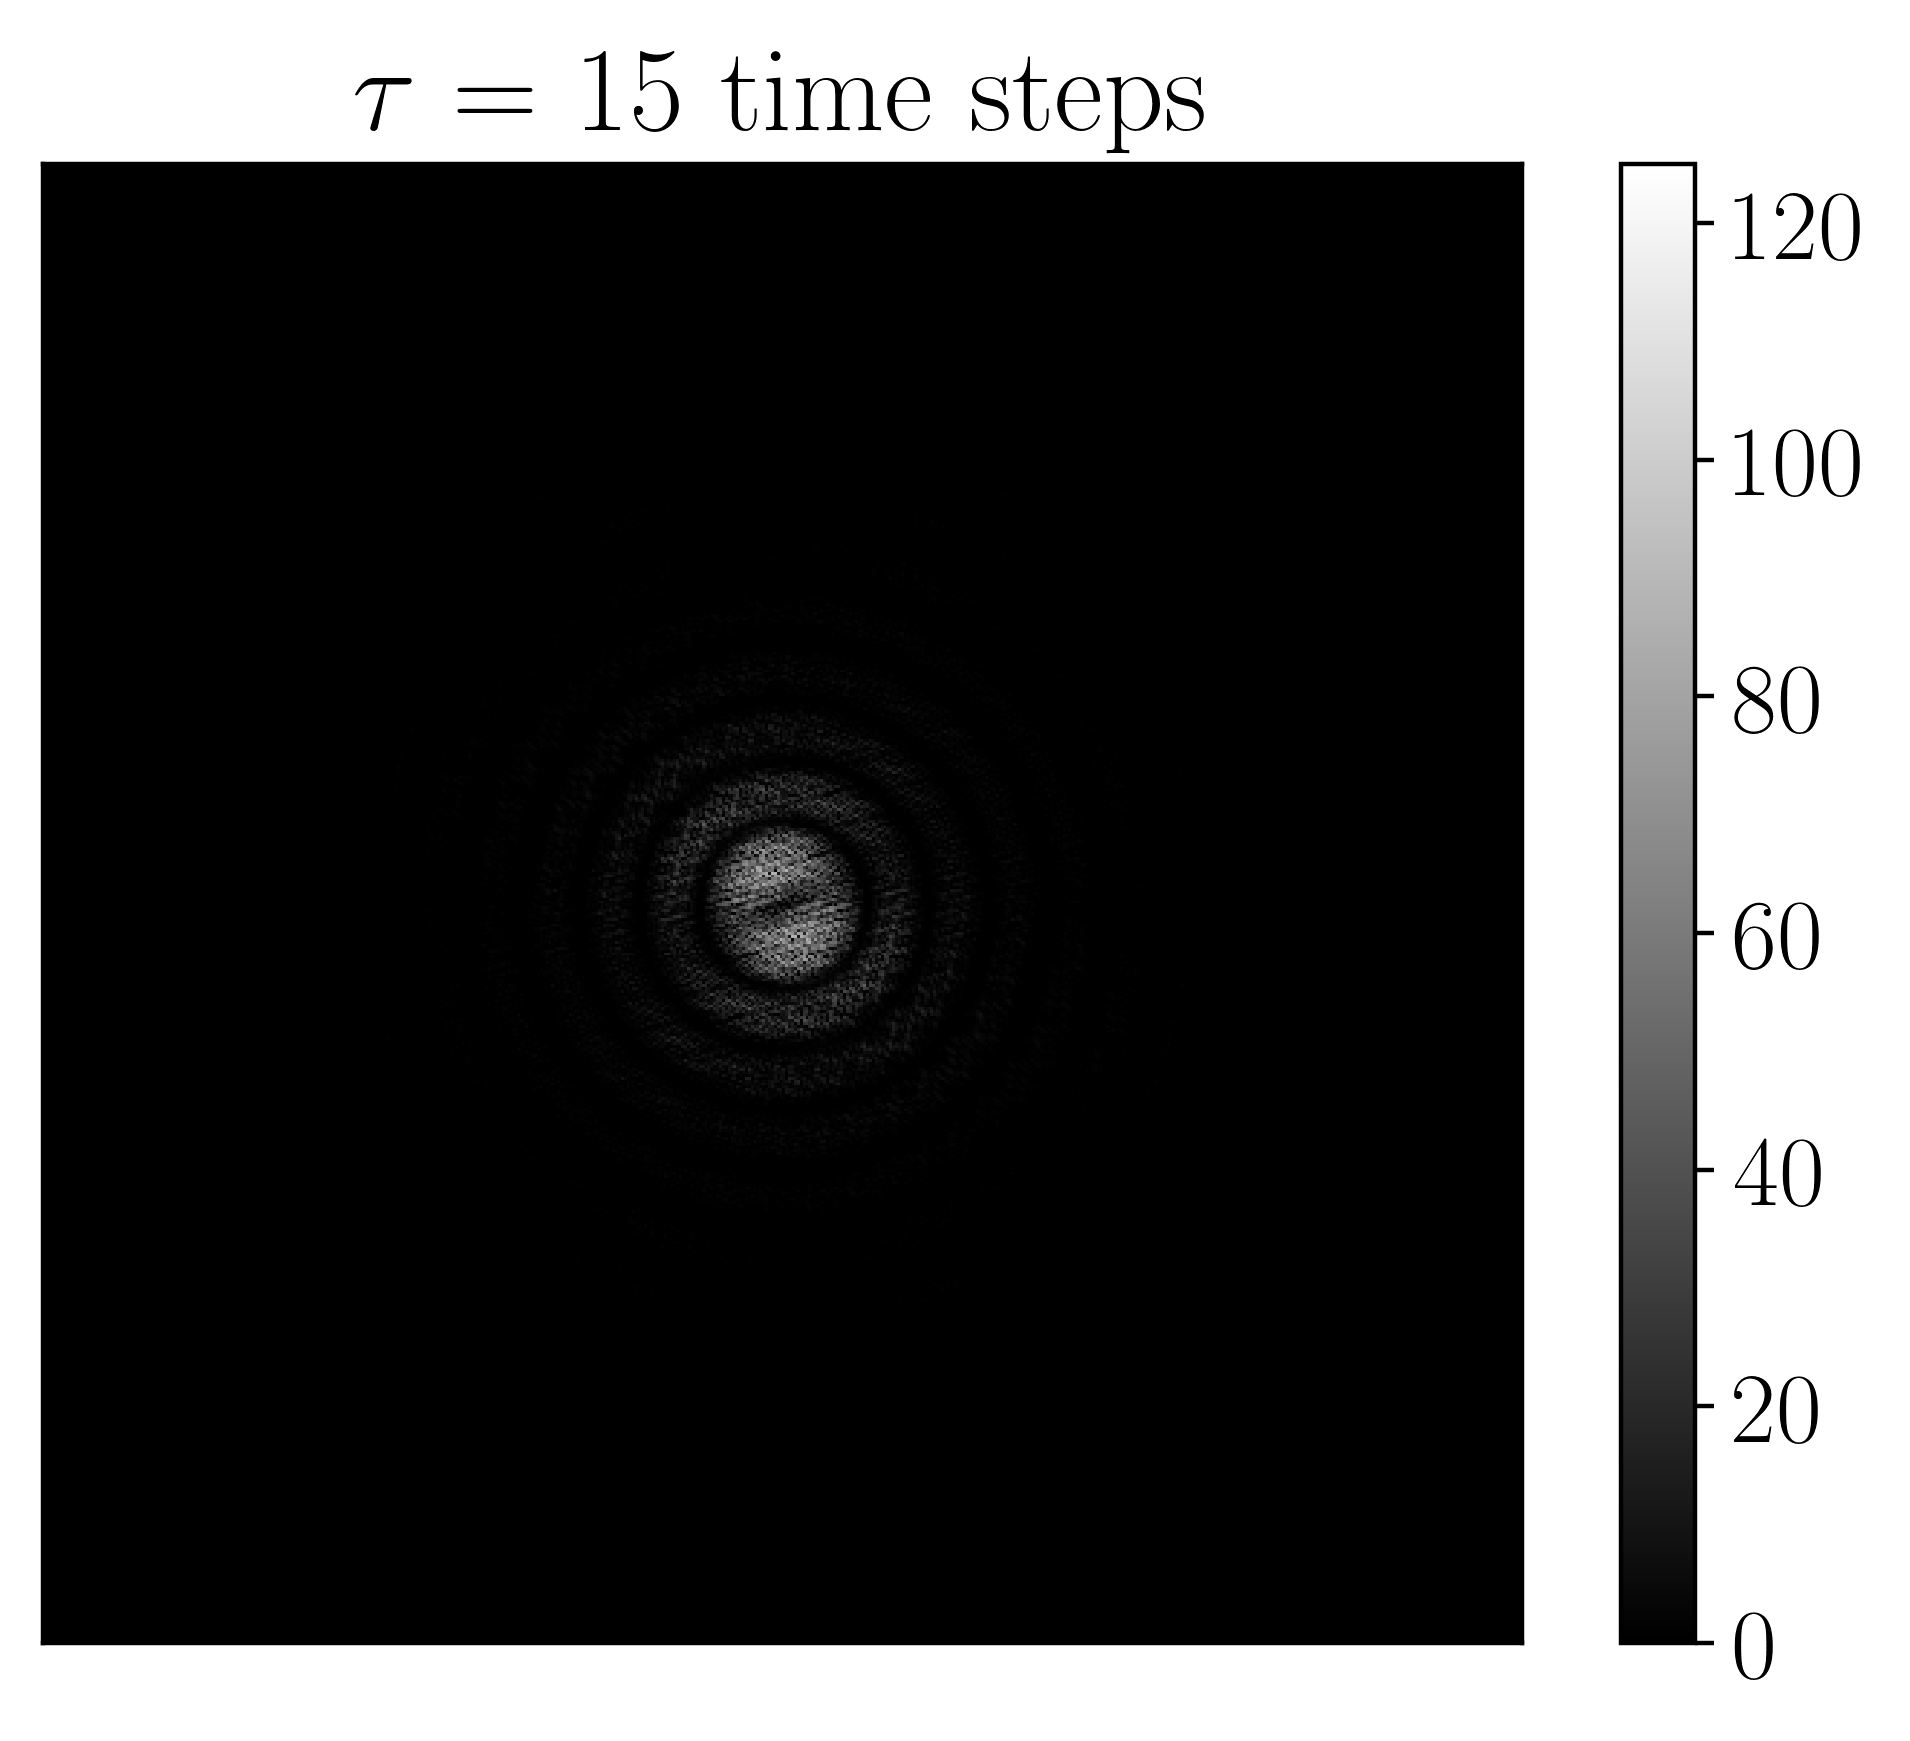
\includegraphics[width=\textwidth]
	{Sources/X-DFA/Mag_Spectrum_d_img_00014.png}}

	\only<6>{
	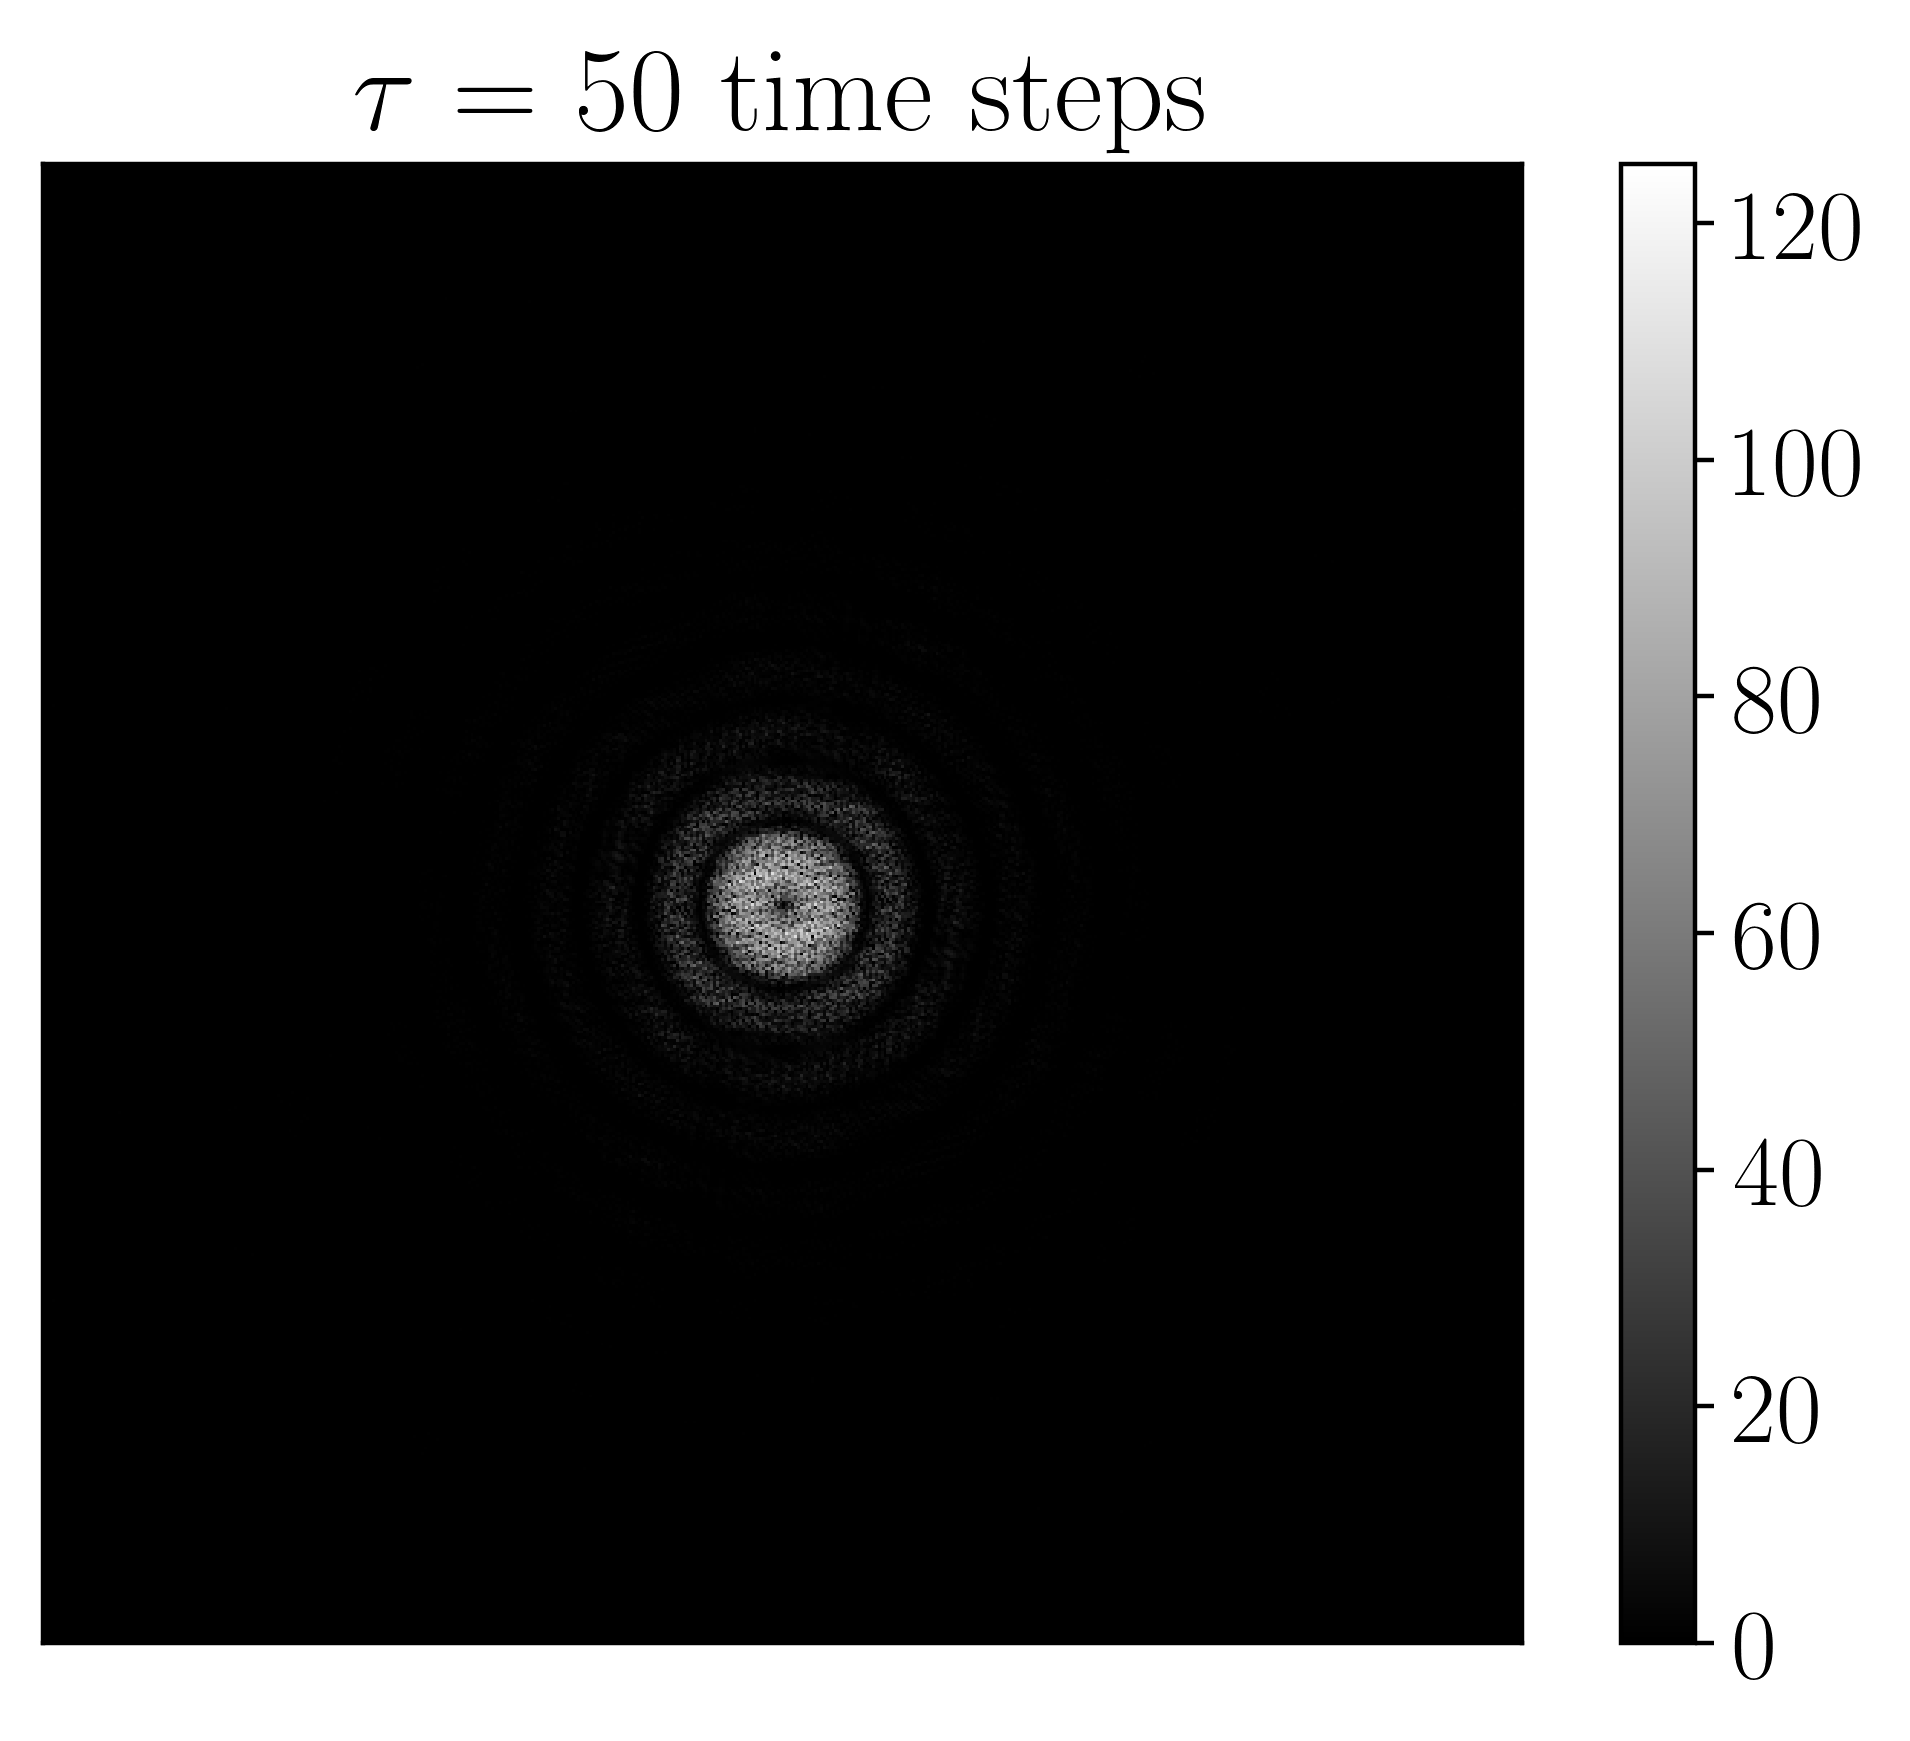
\includegraphics[width=\textwidth]
	{Sources/X-DFA/Mag_Spectrum_d_img_00049.png}}

	\only<7>{
	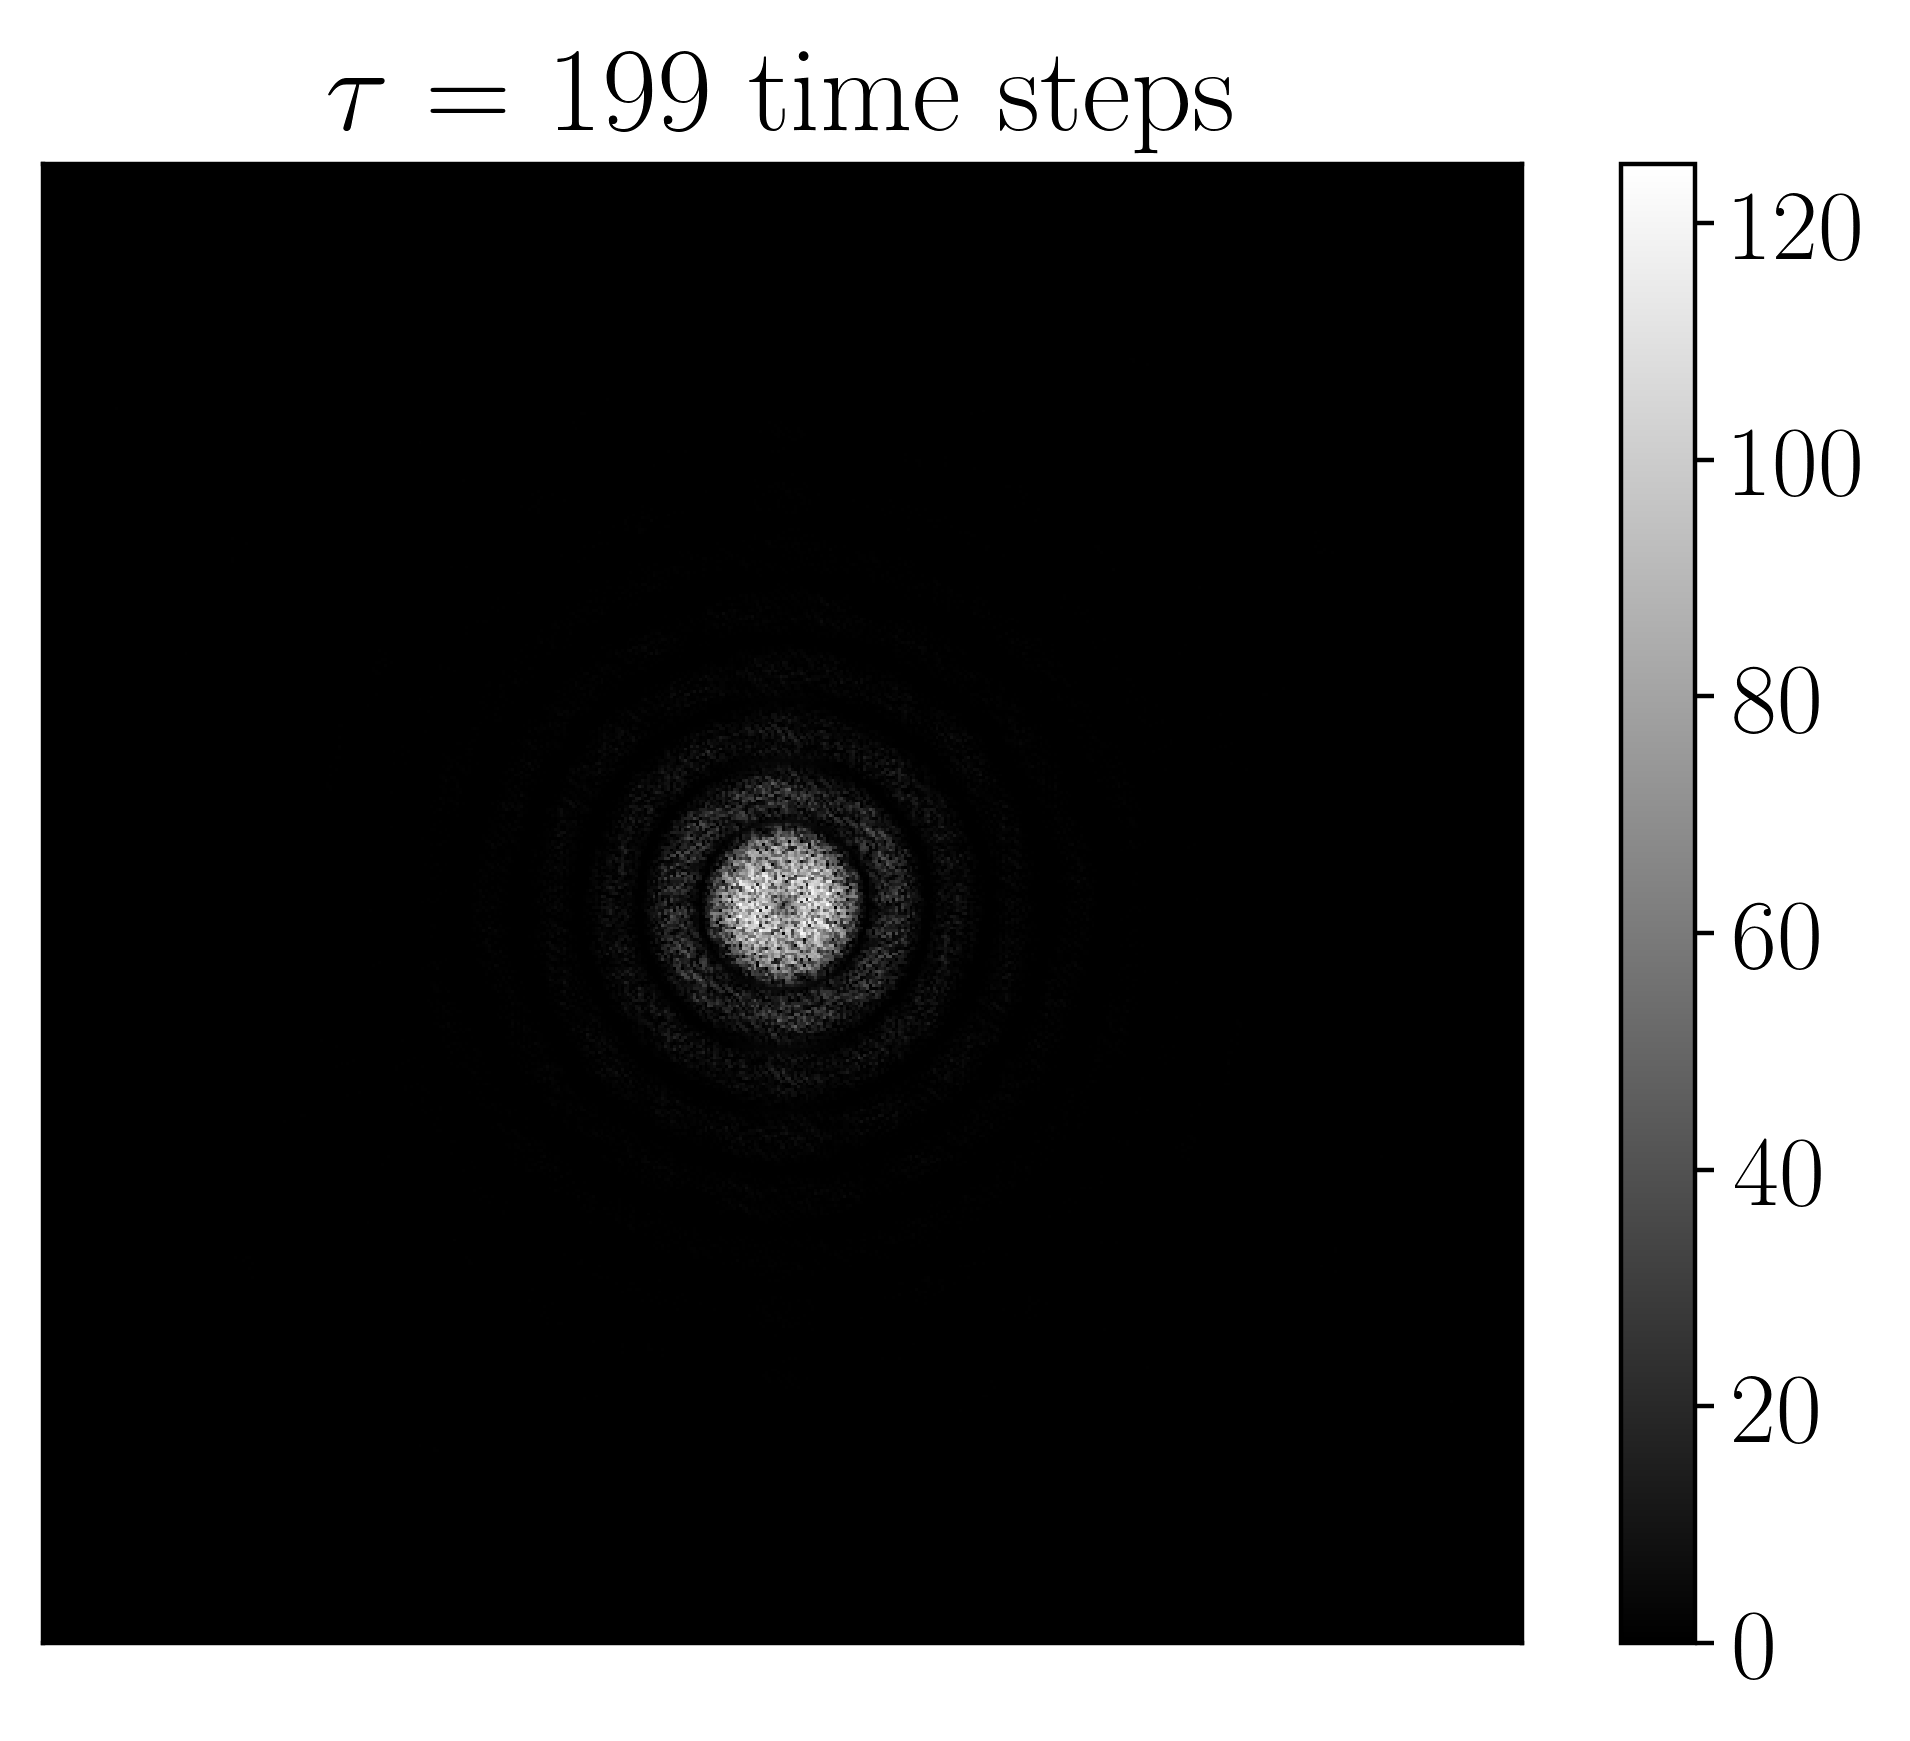
\includegraphics[width=\textwidth]
	{Sources/X-DFA/Mag_Spectrum_d_img_00198.png}}

	\only<8>{
	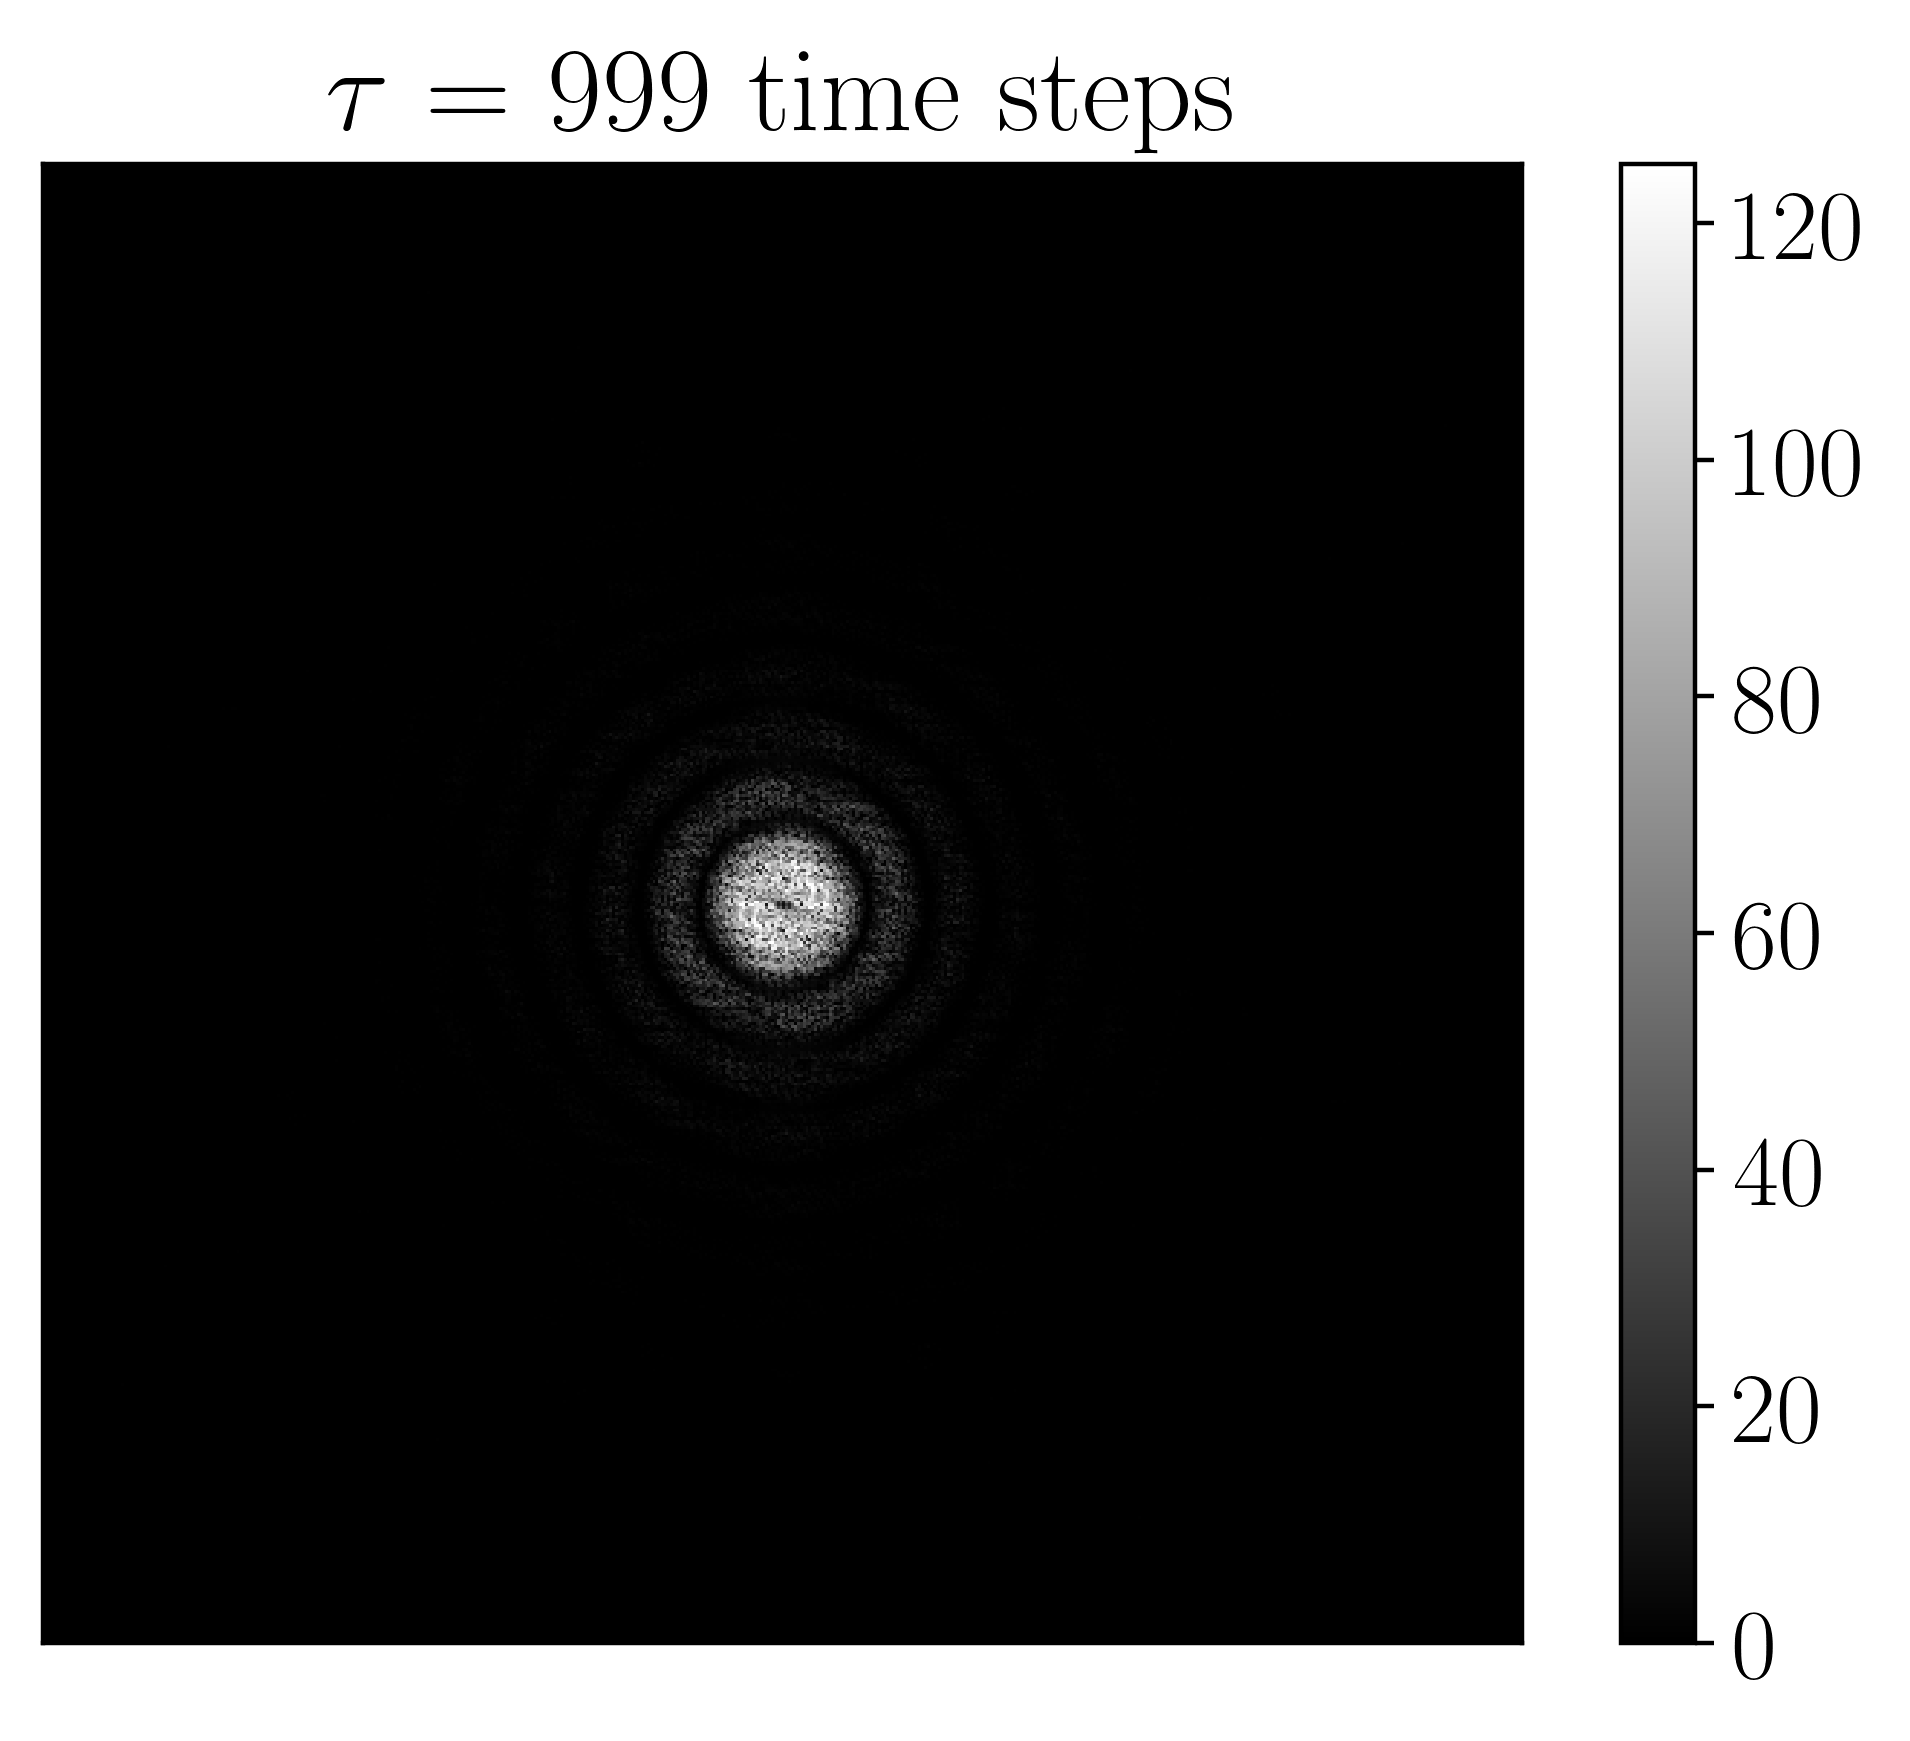
\includegraphics[width=\textwidth]
	{Sources/X-DFA/Mag_Spectrum_d_img_00998.png}}
	\end{textblock}
	
	\begin{textblock}{0.45}(0.5,0.15)
		\centering	
		Time averaging: 
		$D(\mathbf{q},\tau) =  \textcolor{red}{\langle}
		|\mathscr{F}(\Delta I)|^2
		\textcolor{red}{\rangle_t} $\\[0.3cm]
		
		Azimuthal averaging: $D(\mathbf{\textcolor{red}{q}},\tau) \rightarrow D(\textcolor{red}{q},\tau)$ ...
	\end{textblock}

	
	\begin{textblock}{0.5}(0.45,0.35)
	\only<1>{
	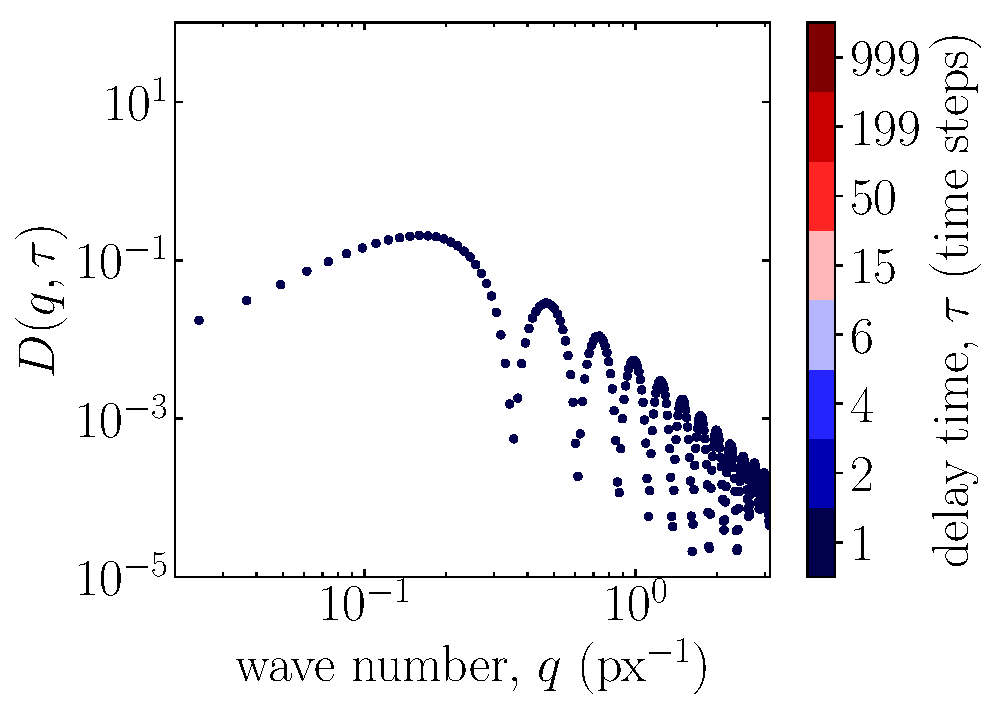
\includegraphics[width=\textwidth]
	{Sources/X-DFA/img_struc_func_vs_q_Ntau1_nPart10.pdf}}
	
	\only<2>{
	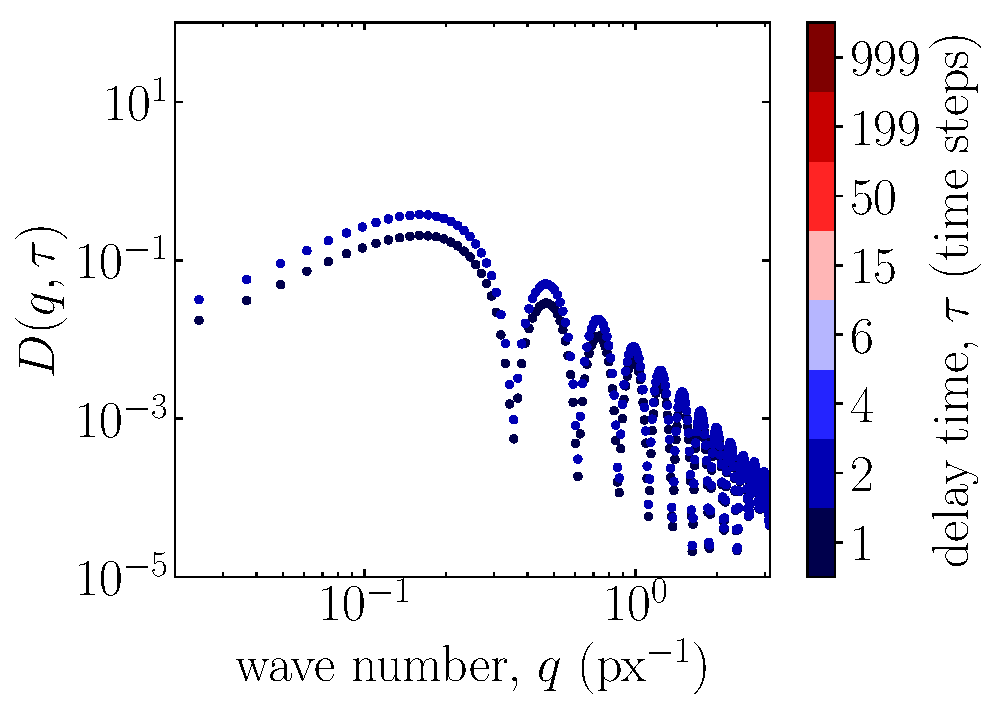
\includegraphics[width=\textwidth]
	{Sources/X-DFA/img_struc_func_vs_q_Ntau2_nPart10.pdf}}

	\only<3>{
	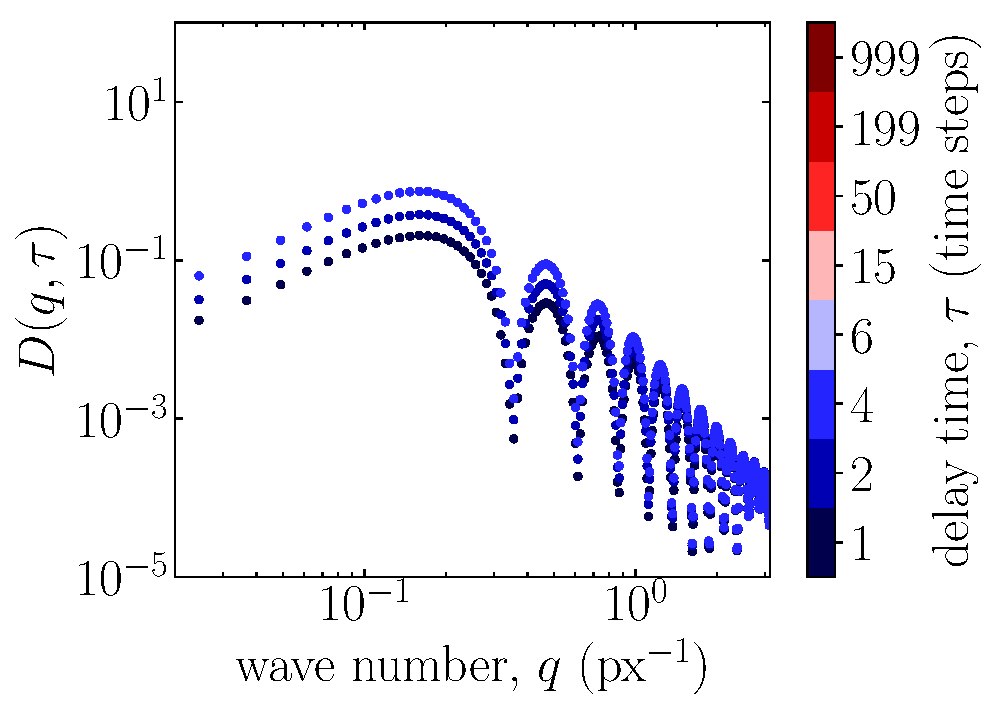
\includegraphics[width=\textwidth]
	{Sources/X-DFA/img_struc_func_vs_q_Ntau4_nPart10.pdf}}

	\only<4>{
	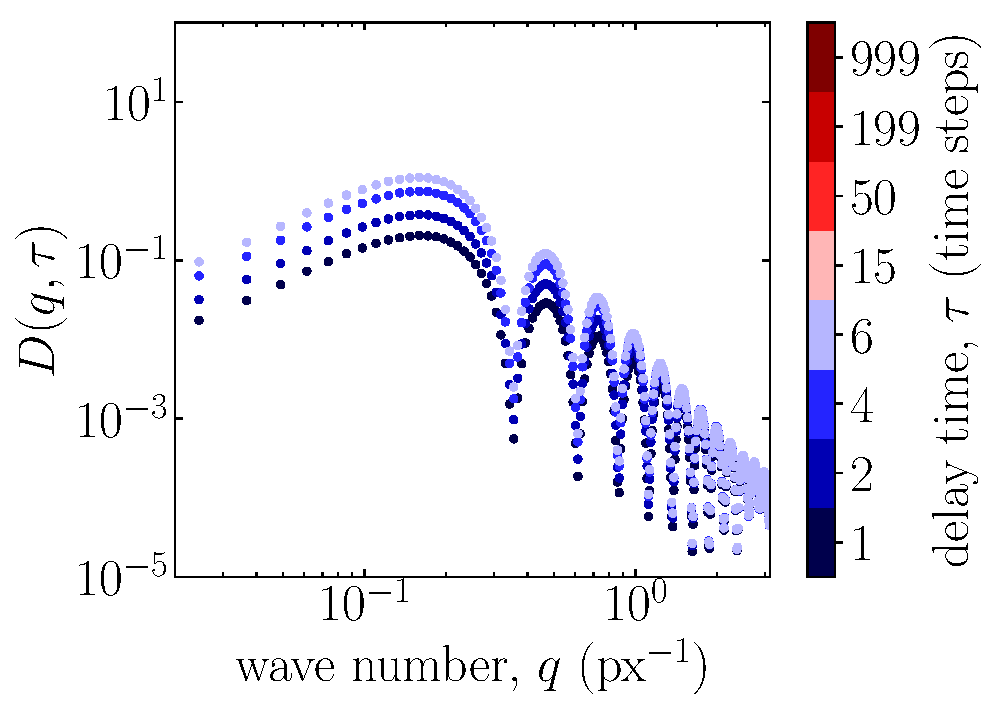
\includegraphics[width=\textwidth]
	{Sources/X-DFA/img_struc_func_vs_q_Ntau6_nPart10.pdf}}

	\only<5>{
	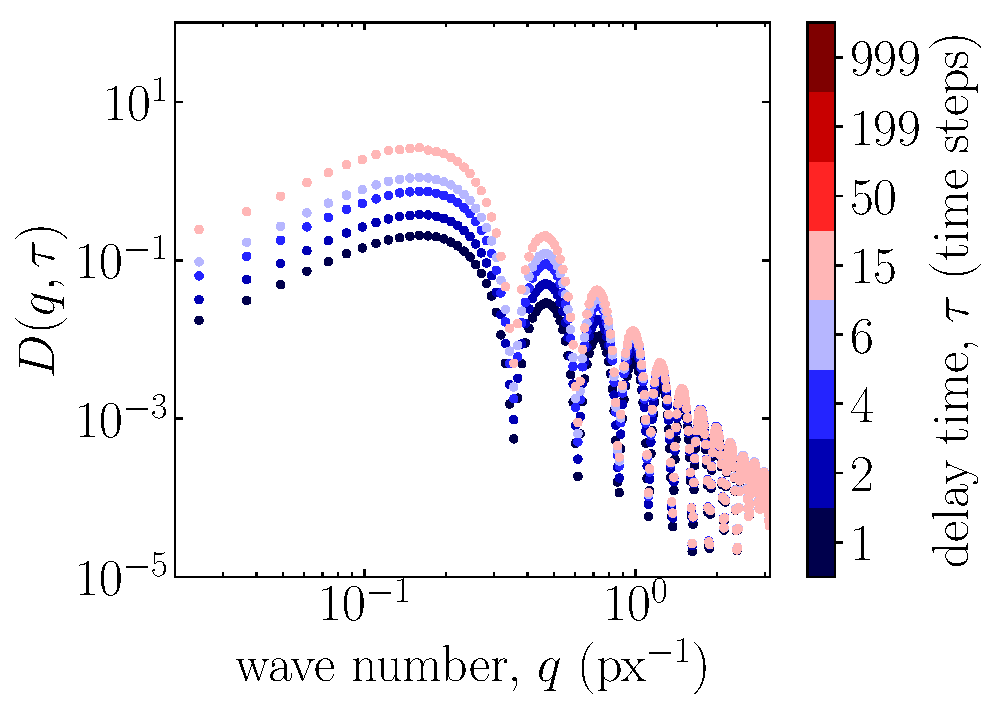
\includegraphics[width=\textwidth]
	{Sources/X-DFA/img_struc_func_vs_q_Ntau15_nPart10.pdf}}

	\only<6>{
	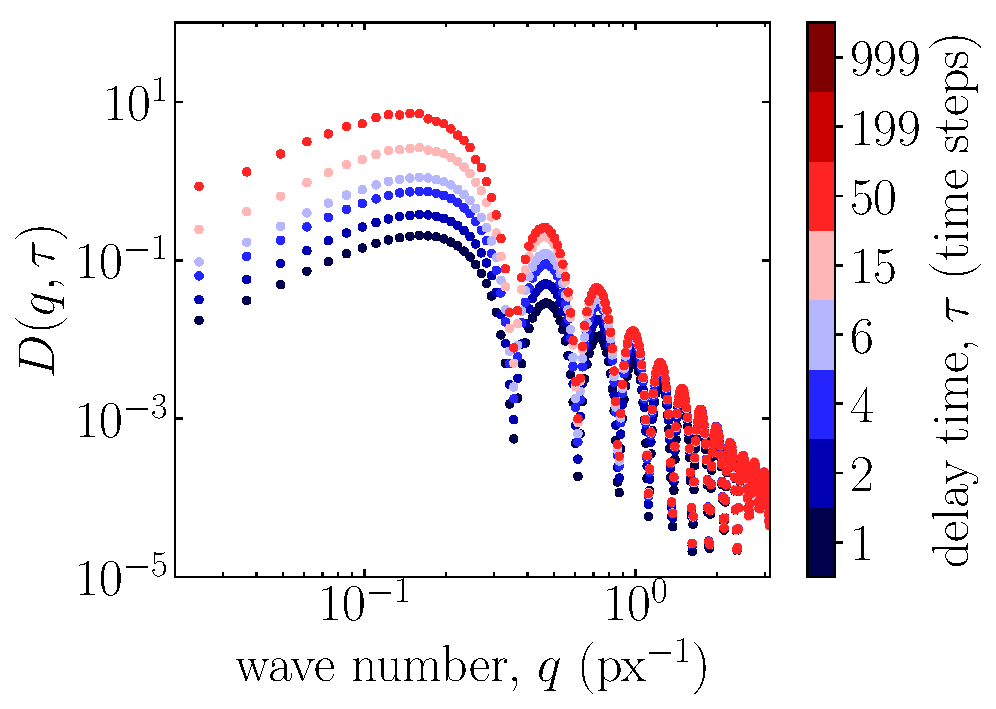
\includegraphics[width=\textwidth]
	{Sources/X-DFA/img_struc_func_vs_q_Ntau50_nPart10.pdf}}

	\only<7>{
	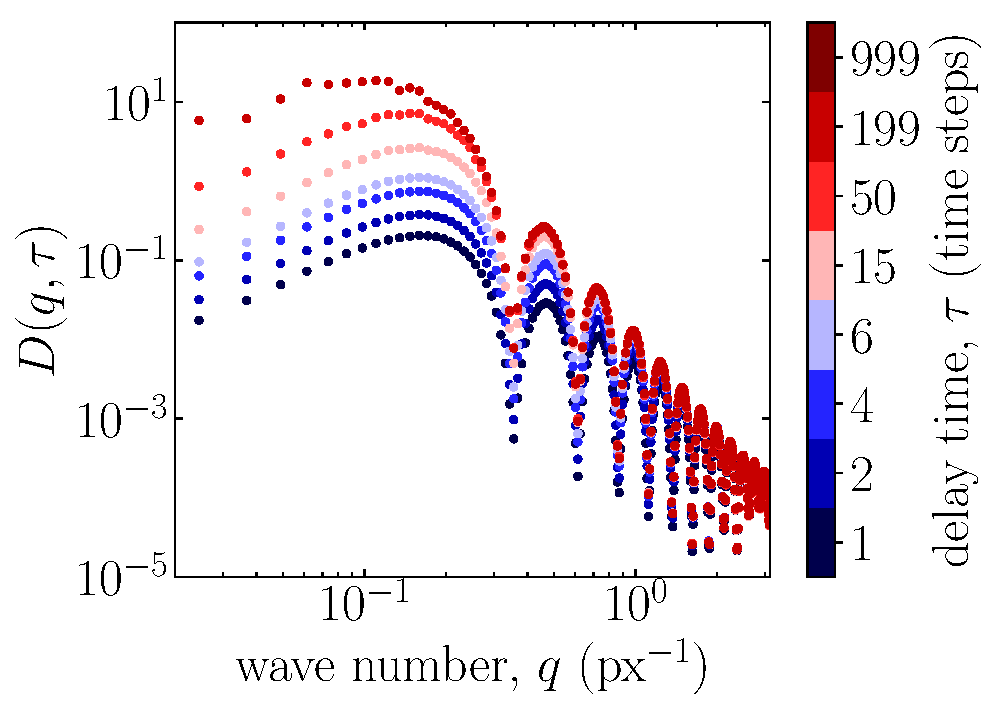
\includegraphics[width=\textwidth]
	{Sources/X-DFA/img_struc_func_vs_q_Ntau199_nPart10.pdf}}

	\only<8>{
	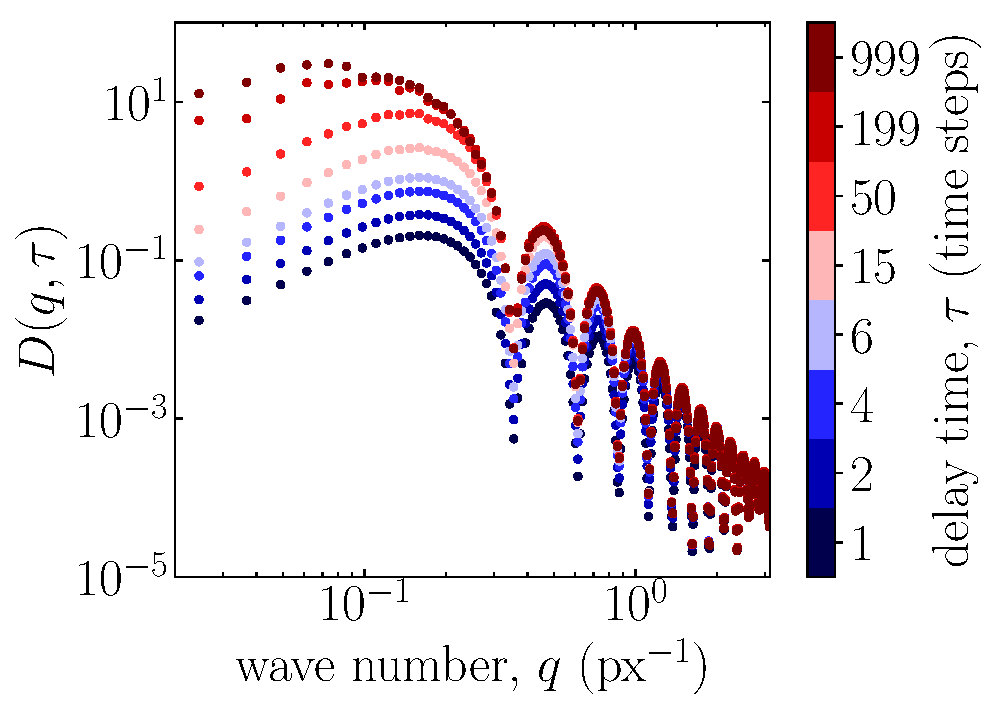
\includegraphics[width=\textwidth]
	{Sources/X-DFA/img_struc_func_vs_q_Ntau999_nPart10.pdf}}
	\end{textblock}

	\begin{textblock}{0.25}(0.05,0.6)
	\centering	
	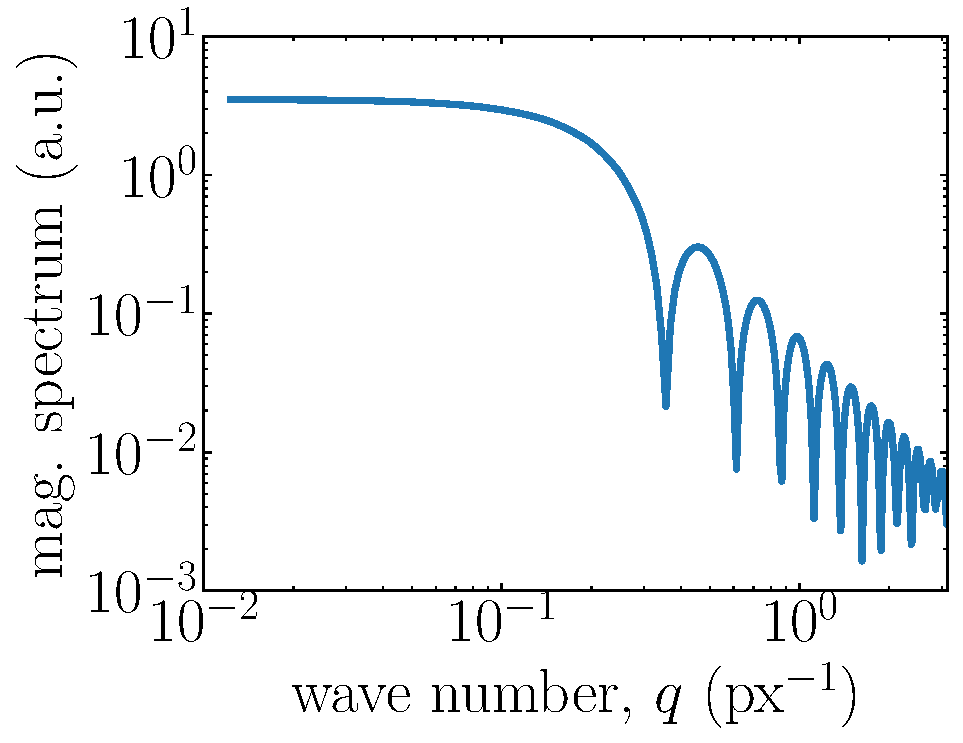
\includegraphics[width=\textwidth]
	{Sources/X-DFA/form_factor.pdf}
	\end{textblock}

	\begin{textblock}{0.06}(0.12,0.7)
	\centering	
	\fbox{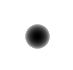
\includegraphics[width=\textwidth]
	{Sources/X-DFA/1Particle_crop_adjust.png}}
	\end{textblock}
%	\begin{textblock}{0.7}(0.05,0.95)
%	\footnotesize{Giavazzi \textit{et al}, PRE \textbf{80}, 031403 (2009)}
%	\end{textblock}
}






%%%%%%%%%%%%%%%%%%%%%%%%%%%%%%%%%
%%%%%%%% d(q,tau) vs tau
\frame{
	\frametitle{The image structure function $D(q,\tau)$}
	\begin{textblock}{0.44}(0.02,0.1)
	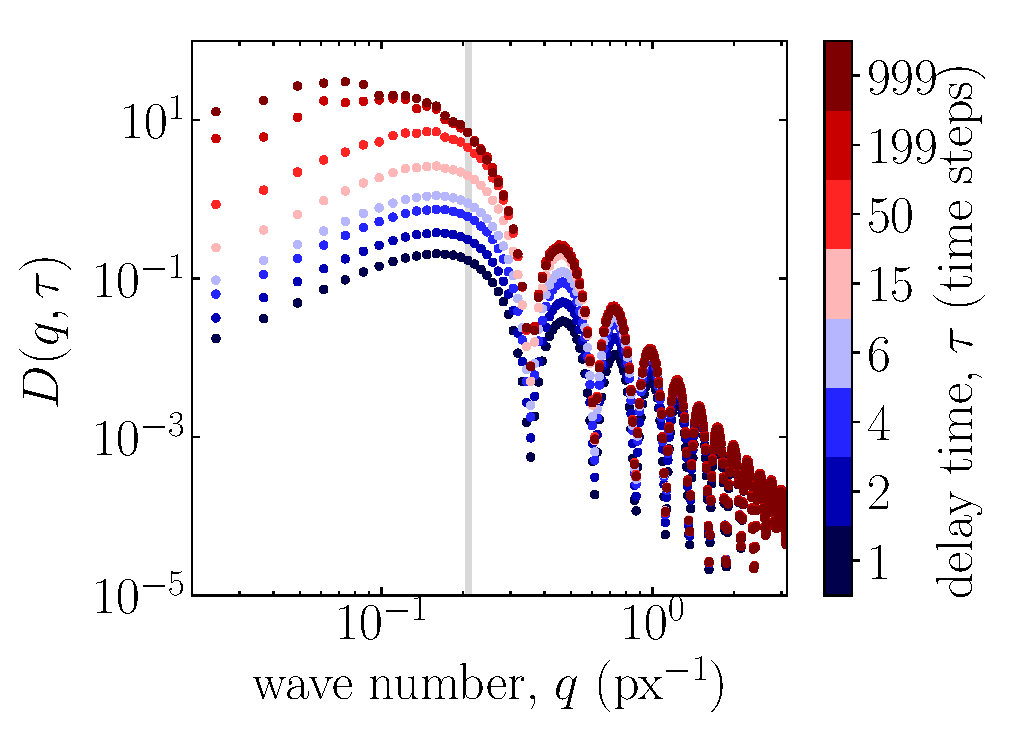
\includegraphics[width=\textwidth]
	{Sources/X-DFA/img_struc_func_vs_q_multiple_tau_simulations_nPart10Marker.eps}
	\end{textblock}

	\begin{textblock}{0.44}(0.52,0.1)
	\only<1>{
	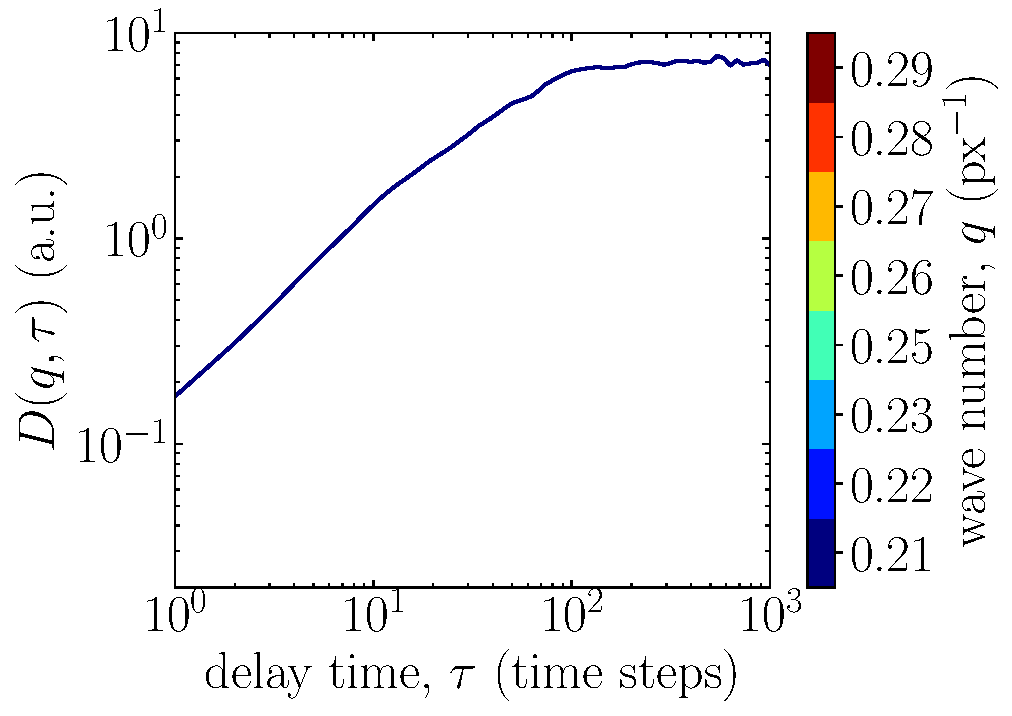
\includegraphics[width=\textwidth]
	{Sources/X-DFA/img_struc_func_vs_tau_q_range_000simulations10.pdf}}

	\only<2>{
	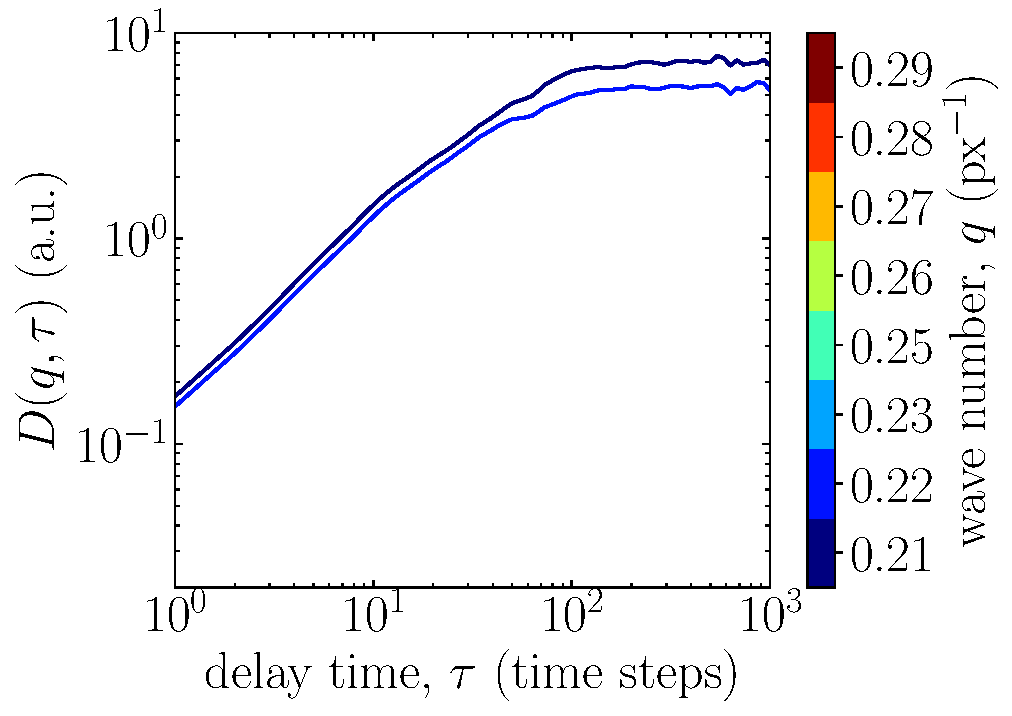
\includegraphics[width=\textwidth]
	{Sources/X-DFA/img_struc_func_vs_tau_q_range_001simulations10.pdf}}

	\only<3>{
	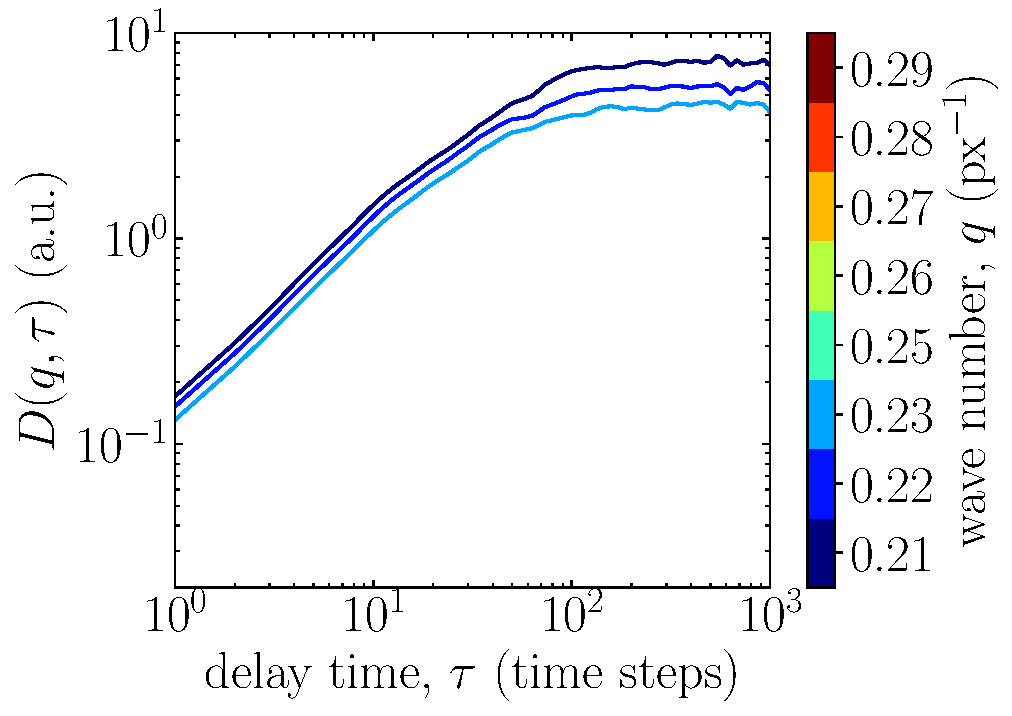
\includegraphics[width=\textwidth]
	{Sources/X-DFA/img_struc_func_vs_tau_q_range_002simulations10.pdf}}

	\visible<4->{
	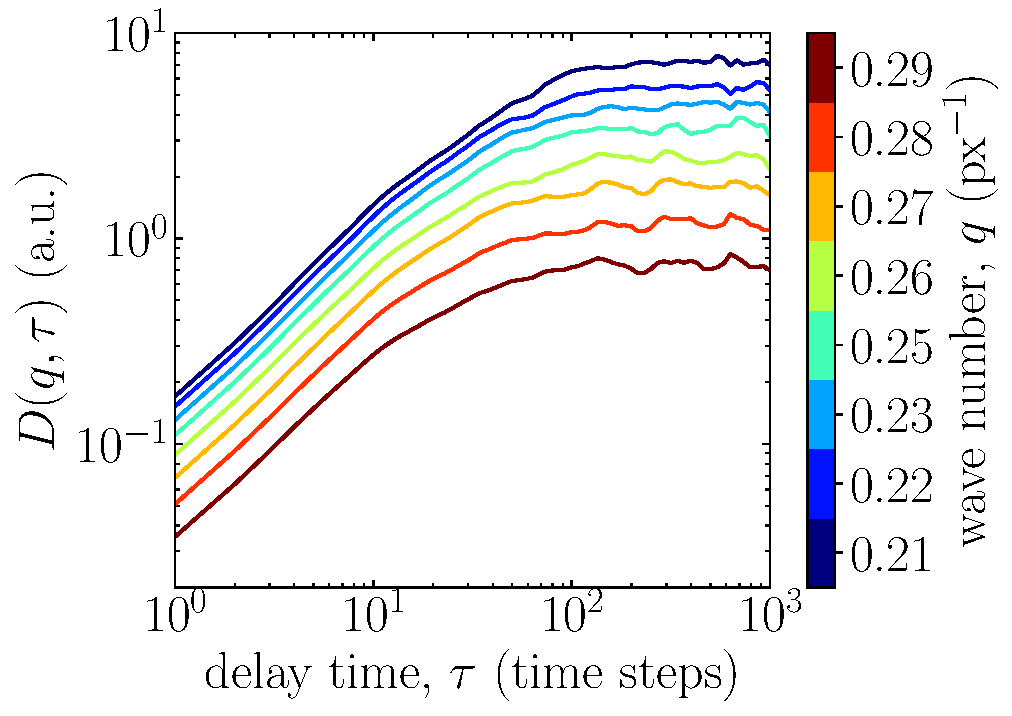
\includegraphics[width=\textwidth]
	{Sources/X-DFA/img_struc_func_vs_tau_q_range_007simulations10.pdf}}
	\end{textblock}


	\begin{textblock}{0.9}(0.05,0.63)
	\centering
	\only<4>{
		\begin{align}
		D(q,\tau)
		&= \Big\langle |I(q, t+\tau) - I(q,t)|^2  \Big\rangle_t \nonumber \\
		&= A(q) 
		\left[1-\frac{\big\langle I^*(q,t) I(q,t+\tau) \big\rangle_t}
		{\big\langle |I(q,t)|^2 \big\rangle_t}\right] 
		+ B(q)\nonumber
		\end{align}
	}
	\end{textblock}

	\begin{textblock}{0.9}(0.05,0.63)
	\visible<5->{
	\begin{align}
	D(q,\tau)
	&= \Big\langle |I(q, t+\tau) - I(q,t)|^2  \Big\rangle_t \nonumber \\
	&= A(q) 
	\bigg[1-
	\textcolor{red}{\underbrace{
			\frac{\big\langle I^*(q,t) I(q,t+\tau) \big\rangle_t}
			{\big\langle |I(q,t)|^2 \big\rangle_t}
	}}
	\bigg] 
	+ B(q)\nonumber
	\end{align}
	}
	\end{textblock}

	\begin{textblock}{0.3}(0.45,0.92)
	\visible<5->{
		\textcolor{red}{Image correlation function}
	}
	\end{textblock}
}


\frame{
\frametitle{Linear space invariant imaging}
	\begin{textblock}{0.5}(0.0,0.15)
	\visible<1->{
	\centering
	Image correlation function
	\[
		g(\mathbf{q}, \tau) = \frac
		{\langle I^*(\mathbf{q},t) I(\mathbf{q},t+\tau) \rangle_t}
		{\langle |I(\mathbf{q},t)|^2 \rangle_t}
	\]
	}
	\end{textblock}



	\begin{textblock}{0.5}(0.5,0.15)
	\visible<2->{
	\centering
	Intermediate scattering function
	\[
		f(\mathbf{q},\tau) = \frac
		{\langle \rho^*(\mathbf{q},t) \rho(\mathbf{q},t+\tau) \rangle_t}
		{\langle |\rho(\mathbf{q},t)|^2 \rangle_t}
	\]}
	\end{textblock}

	\begin{textblock}{0.9}(0.05,0.42)
		\visible<2->{	
		Linear space-invariant imaging:
		\begin{align}
		I(\mathbf{r},t) = I_0 + \int \mathsf{d}\mathbf{r}' \ \mathsf{d}z'
		T(\mathbf{r}-\mathbf{r}',-z') c(\mathbf{r}',z',t)
		\nonumber
		\end{align}
		}
	\end{textblock}


	\begin{textblock}{0.9}(0.05,0.6)
	\visible<2->{
		\centering
		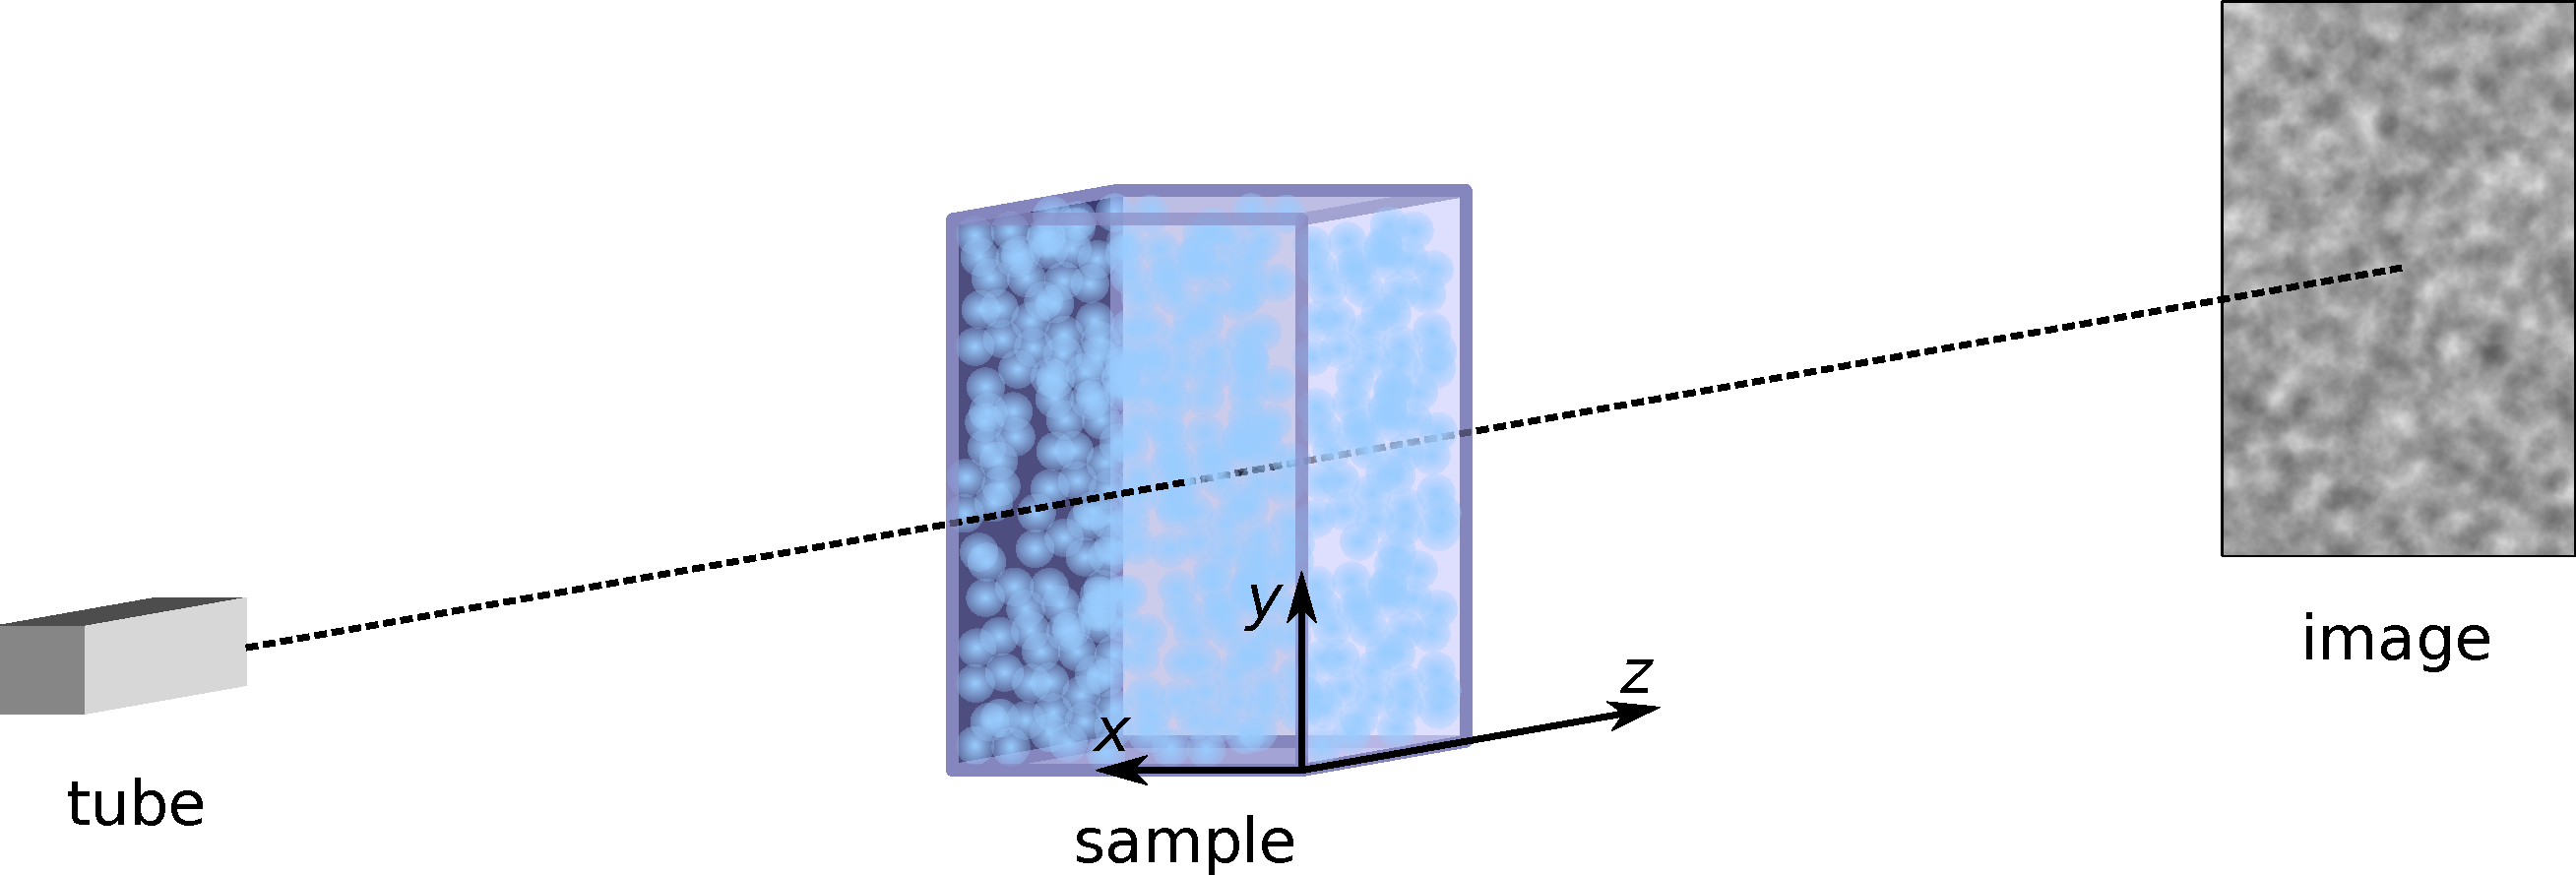
\includegraphics[width=0.7\textwidth]
		{Sources/X-DFA/image_transfer_function1.pdf}
	}
	\end{textblock}
	
}

\frame{
%\frametitle{Intermediate Scattering Function}

\begin{textblock}{0.38}(0.02,0.02)
	\only<1>{
	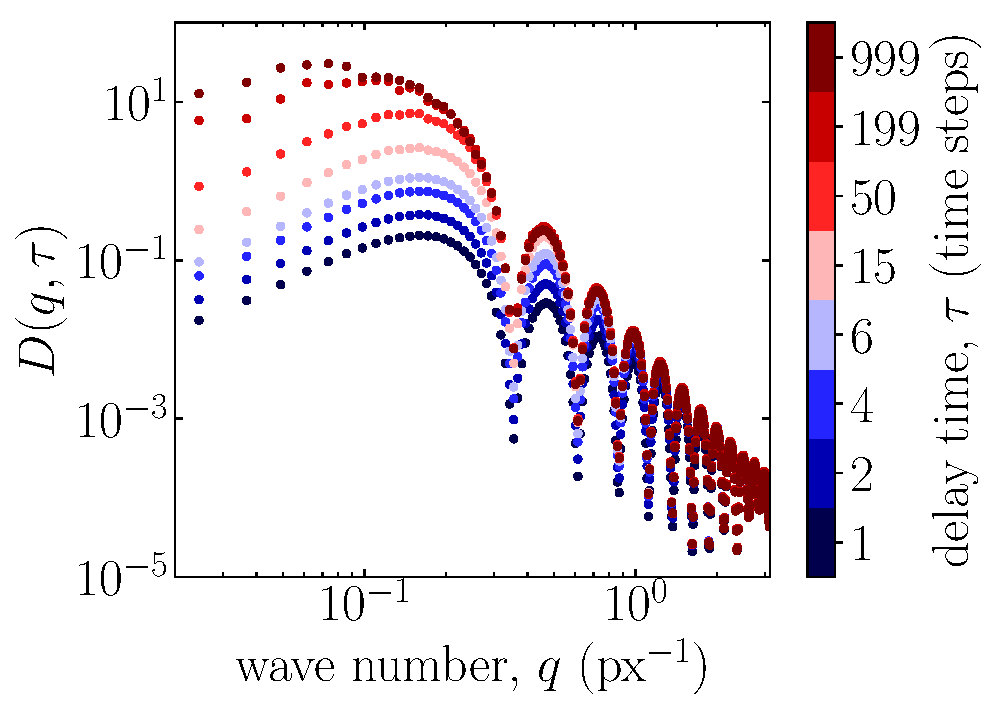
\includegraphics[width=\textwidth]
	{Sources/X-DFA/img_struc_func_vs_q_Ntau999_nPart10.pdf}}

	\visible<2->{
	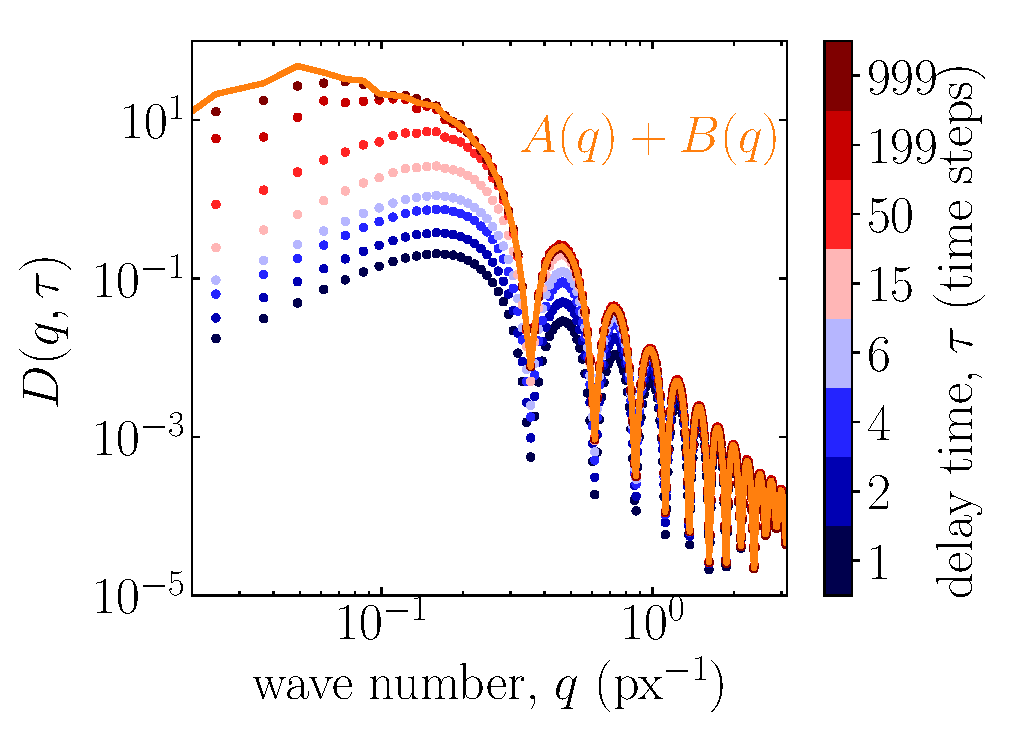
\includegraphics[width=\textwidth]
	{Sources/X-DFA/img_struc_func_vs_q_multiple_tau_simulations_nPart10with_A.eps}}
\end{textblock}

\begin{textblock}{0.38}(0.55,0.02)
	\visible<1->{
		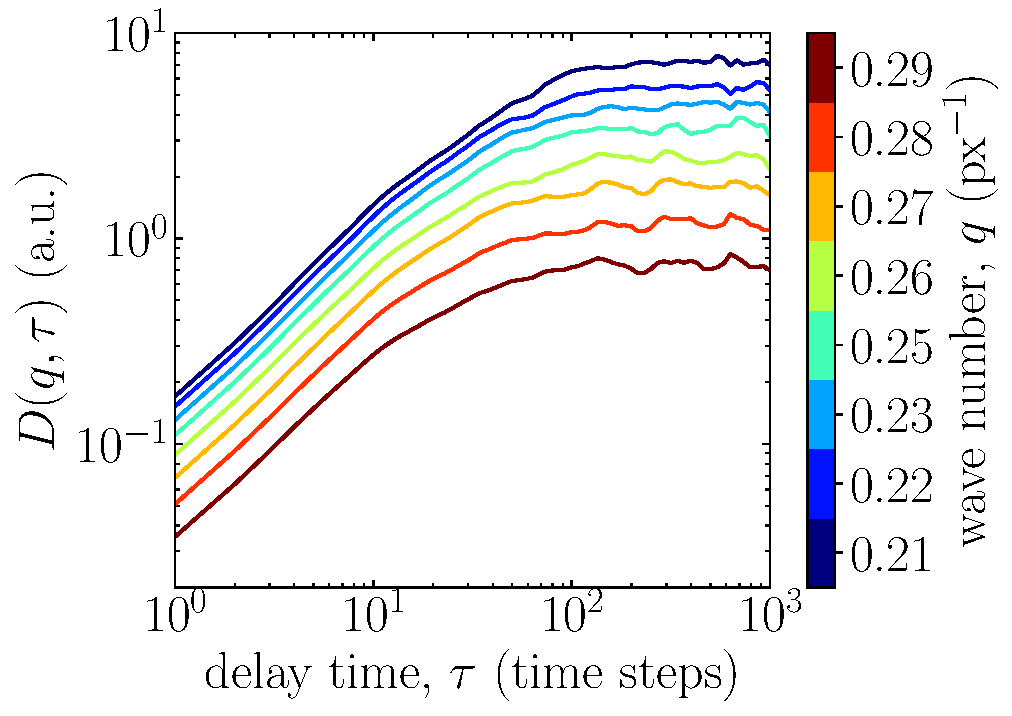
\includegraphics[width=\textwidth]
		{Sources/X-DFA/img_struc_func_vs_tau_q_range_007simulations10.pdf}}
\end{textblock}



\begin{textblock}{0.5}(0.02,0.5)
	\only<1>{
	\begin{align}
	D(q,\tau)
	&= \Big\langle |I(q, t+\tau) - I(q,t)|^2  \Big\rangle_t \nonumber \\
	&= A(q) 
	\bigg[1-
	\textcolor{red}{\underbrace{
			\frac{\big\langle I^*(q,t) I(q,t+\tau) \big\rangle_t}
			{\big\langle |I(q,t)|^2 \big\rangle_t}
	}}
	\bigg] 
	+ B(q)\nonumber
	\end{align}
	}
\end{textblock}

\begin{textblock}{0.3}(0.2,0.8)
	\only<1>{
		\textcolor{red}{Image correlation function}
	}
\end{textblock}

\begin{textblock}{0.5}(0.02,0.5)
	\visible<2->{
		\begin{align}
		D(q,\tau)
		&= \Big\langle |I(q, t+\tau) - I(q,t)|^2  \Big\rangle_t \nonumber \\
		&= \textcolor{orange}{A(q)}
		\bigg[1-
		\textcolor{red}{
				\frac{\big\langle I^*(q,t) I(q,t+\tau) \big\rangle_t}
				{\big\langle |I(q,t)|^2 \big\rangle_t}
		}
		\bigg] 
		+ \textcolor{darkgreen}{B(q)}\nonumber
		\end{align}
		
	\begin{itemize}
		\item $D(q, \tau \rightarrow 0) = \textcolor{darkgreen}{B(q)} = 0$
		\item $D(q, \tau \rightarrow \infty) = A(q) + B(q)$
	\end{itemize}
	}
\end{textblock}


\begin{textblock}{0.38}(0.55,0.5)
	\visible<3->{
		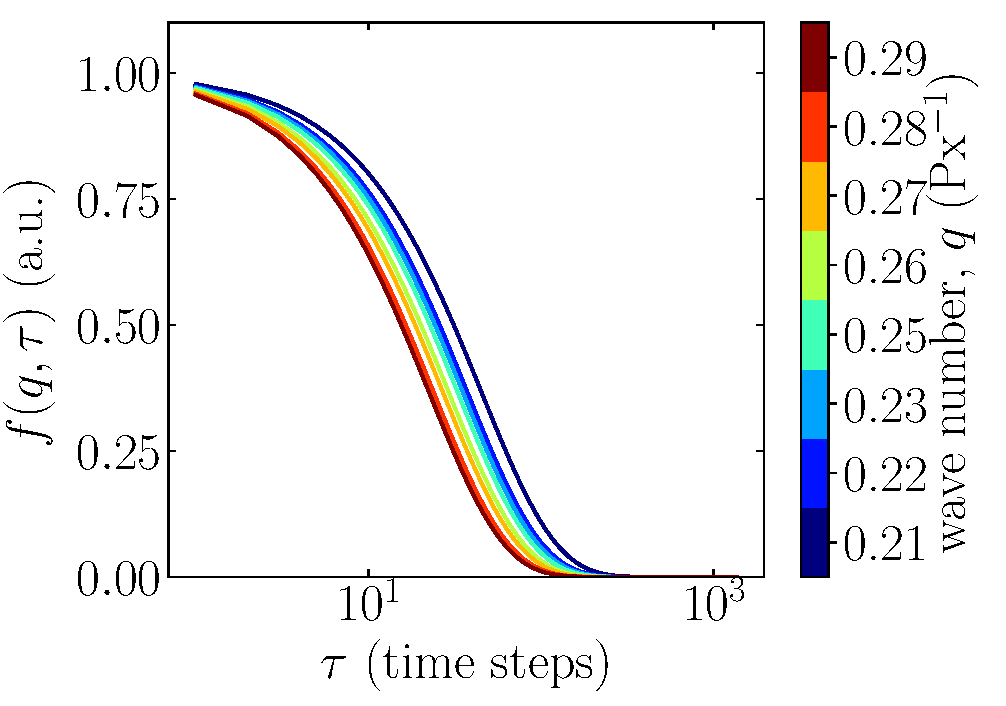
\includegraphics[width=\textwidth]
		{Sources/X-DFA/ISF_vs_tau.pdf}}
\end{textblock}

}

\frame{
\frametitle{Intermediate scattering function $f(q,\tau)$}

\begin{textblock}{0.35}(0.02,0.1)
	\visible<1->{
		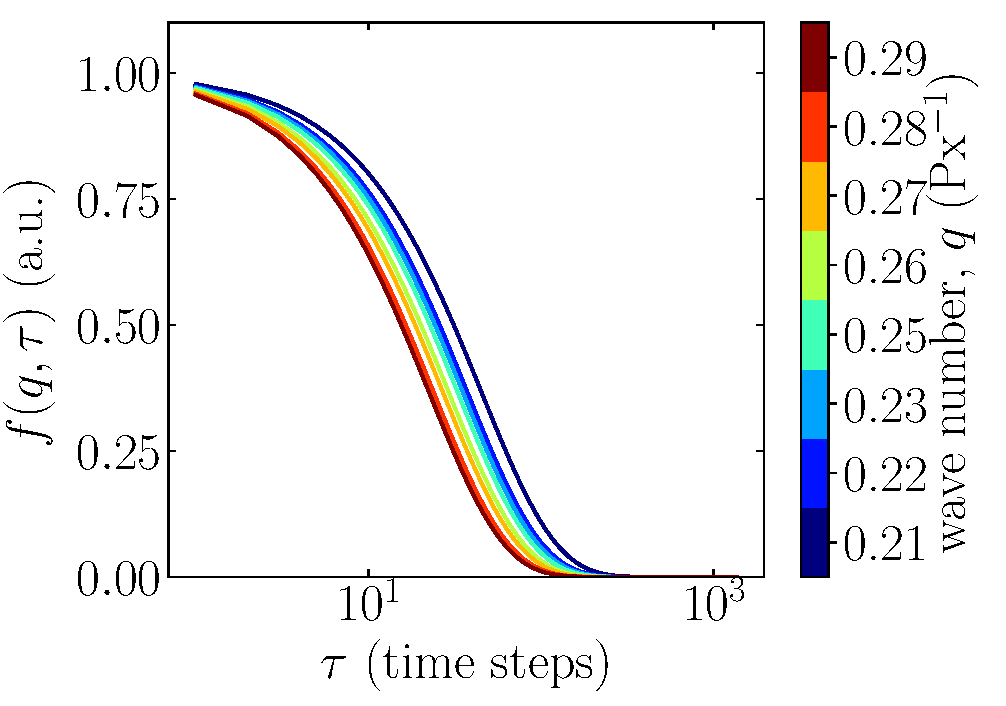
\includegraphics[width=\textwidth]
		{Sources/X-DFA/ISF_vs_tau.pdf}}
\end{textblock}



\begin{textblock}{0.35}(0.02,0.55)
	\visible<1->{
		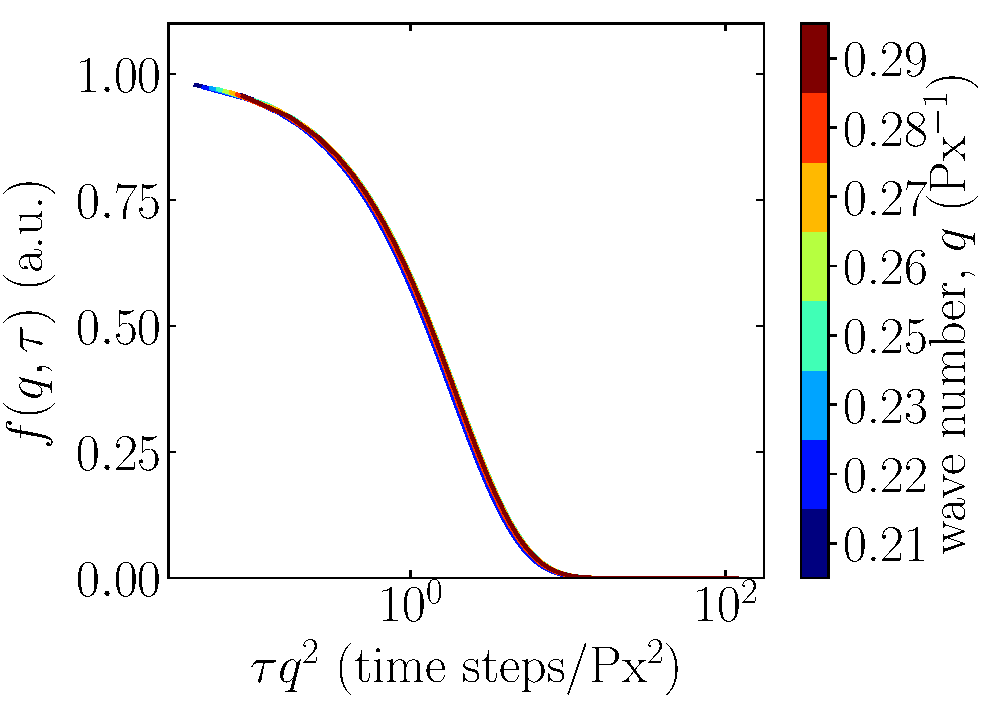
\includegraphics[width=\textwidth]
		{Sources/X-DFA/ISF_vs_tau_q_squared.pdf}}
\end{textblock}

\begin{textblock}{0.5}(0.4,0.15)
	\centering
	\visible<1->{
		Brownian motion:\\
		$f(q,\tau) = \exp(- q^2 \tau/\tau_\text{D})$\\
		Accuracy: 2\% - 6\%
	}
\end{textblock}

\begin{textblock}{0.5}(0.4,0.33)
	\visible<1->{
		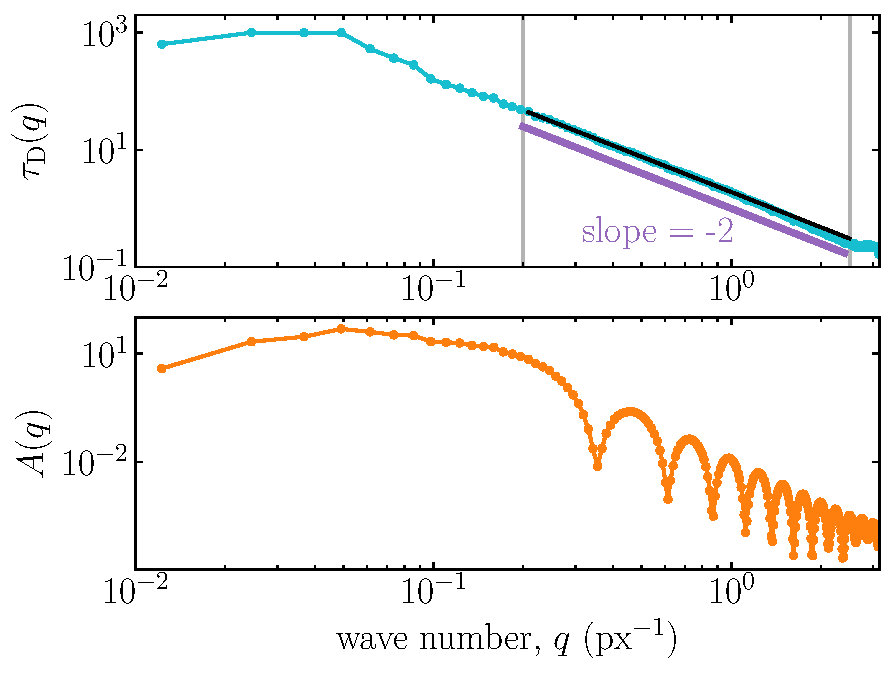
\includegraphics[width=\textwidth]
		{Sources/X-DFA/FitParameters.pdf}}
\end{textblock}
}

\frame{
\textcolor{red}{extra slide with videos of 10, 1000, 100000 particles + accuracy,
next slide is \textit{Extending DDM to X-DFA}}
}

